% Options for packages loaded elsewhere
\PassOptionsToPackage{unicode}{hyperref}
\PassOptionsToPackage{hyphens}{url}
%
\documentclass[
]{book}
\usepackage{amsmath,amssymb}
\usepackage{lmodern}
\usepackage{ifxetex,ifluatex}
\ifnum 0\ifxetex 1\fi\ifluatex 1\fi=0 % if pdftex
  \usepackage[T1]{fontenc}
  \usepackage[utf8]{inputenc}
  \usepackage{textcomp} % provide euro and other symbols
\else % if luatex or xetex
  \usepackage{unicode-math}
  \defaultfontfeatures{Scale=MatchLowercase}
  \defaultfontfeatures[\rmfamily]{Ligatures=TeX,Scale=1}
\fi
% Use upquote if available, for straight quotes in verbatim environments
\IfFileExists{upquote.sty}{\usepackage{upquote}}{}
\IfFileExists{microtype.sty}{% use microtype if available
  \usepackage[]{microtype}
  \UseMicrotypeSet[protrusion]{basicmath} % disable protrusion for tt fonts
}{}
\makeatletter
\@ifundefined{KOMAClassName}{% if non-KOMA class
  \IfFileExists{parskip.sty}{%
    \usepackage{parskip}
  }{% else
    \setlength{\parindent}{0pt}
    \setlength{\parskip}{6pt plus 2pt minus 1pt}}
}{% if KOMA class
  \KOMAoptions{parskip=half}}
\makeatother
\usepackage{xcolor}
\IfFileExists{xurl.sty}{\usepackage{xurl}}{} % add URL line breaks if available
\IfFileExists{bookmark.sty}{\usepackage{bookmark}}{\usepackage{hyperref}}
\hypersetup{
  pdftitle={Statistical methods for environmental mixtures},
  pdfauthor={Andrea Bellavia},
  hidelinks,
  pdfcreator={LaTeX via pandoc}}
\urlstyle{same} % disable monospaced font for URLs
\usepackage{color}
\usepackage{fancyvrb}
\newcommand{\VerbBar}{|}
\newcommand{\VERB}{\Verb[commandchars=\\\{\}]}
\DefineVerbatimEnvironment{Highlighting}{Verbatim}{commandchars=\\\{\}}
% Add ',fontsize=\small' for more characters per line
\usepackage{framed}
\definecolor{shadecolor}{RGB}{248,248,248}
\newenvironment{Shaded}{\begin{snugshade}}{\end{snugshade}}
\newcommand{\AlertTok}[1]{\textcolor[rgb]{0.94,0.16,0.16}{#1}}
\newcommand{\AnnotationTok}[1]{\textcolor[rgb]{0.56,0.35,0.01}{\textbf{\textit{#1}}}}
\newcommand{\AttributeTok}[1]{\textcolor[rgb]{0.77,0.63,0.00}{#1}}
\newcommand{\BaseNTok}[1]{\textcolor[rgb]{0.00,0.00,0.81}{#1}}
\newcommand{\BuiltInTok}[1]{#1}
\newcommand{\CharTok}[1]{\textcolor[rgb]{0.31,0.60,0.02}{#1}}
\newcommand{\CommentTok}[1]{\textcolor[rgb]{0.56,0.35,0.01}{\textit{#1}}}
\newcommand{\CommentVarTok}[1]{\textcolor[rgb]{0.56,0.35,0.01}{\textbf{\textit{#1}}}}
\newcommand{\ConstantTok}[1]{\textcolor[rgb]{0.00,0.00,0.00}{#1}}
\newcommand{\ControlFlowTok}[1]{\textcolor[rgb]{0.13,0.29,0.53}{\textbf{#1}}}
\newcommand{\DataTypeTok}[1]{\textcolor[rgb]{0.13,0.29,0.53}{#1}}
\newcommand{\DecValTok}[1]{\textcolor[rgb]{0.00,0.00,0.81}{#1}}
\newcommand{\DocumentationTok}[1]{\textcolor[rgb]{0.56,0.35,0.01}{\textbf{\textit{#1}}}}
\newcommand{\ErrorTok}[1]{\textcolor[rgb]{0.64,0.00,0.00}{\textbf{#1}}}
\newcommand{\ExtensionTok}[1]{#1}
\newcommand{\FloatTok}[1]{\textcolor[rgb]{0.00,0.00,0.81}{#1}}
\newcommand{\FunctionTok}[1]{\textcolor[rgb]{0.00,0.00,0.00}{#1}}
\newcommand{\ImportTok}[1]{#1}
\newcommand{\InformationTok}[1]{\textcolor[rgb]{0.56,0.35,0.01}{\textbf{\textit{#1}}}}
\newcommand{\KeywordTok}[1]{\textcolor[rgb]{0.13,0.29,0.53}{\textbf{#1}}}
\newcommand{\NormalTok}[1]{#1}
\newcommand{\OperatorTok}[1]{\textcolor[rgb]{0.81,0.36,0.00}{\textbf{#1}}}
\newcommand{\OtherTok}[1]{\textcolor[rgb]{0.56,0.35,0.01}{#1}}
\newcommand{\PreprocessorTok}[1]{\textcolor[rgb]{0.56,0.35,0.01}{\textit{#1}}}
\newcommand{\RegionMarkerTok}[1]{#1}
\newcommand{\SpecialCharTok}[1]{\textcolor[rgb]{0.00,0.00,0.00}{#1}}
\newcommand{\SpecialStringTok}[1]{\textcolor[rgb]{0.31,0.60,0.02}{#1}}
\newcommand{\StringTok}[1]{\textcolor[rgb]{0.31,0.60,0.02}{#1}}
\newcommand{\VariableTok}[1]{\textcolor[rgb]{0.00,0.00,0.00}{#1}}
\newcommand{\VerbatimStringTok}[1]{\textcolor[rgb]{0.31,0.60,0.02}{#1}}
\newcommand{\WarningTok}[1]{\textcolor[rgb]{0.56,0.35,0.01}{\textbf{\textit{#1}}}}
\usepackage{longtable,booktabs,array}
\usepackage{calc} % for calculating minipage widths
% Correct order of tables after \paragraph or \subparagraph
\usepackage{etoolbox}
\makeatletter
\patchcmd\longtable{\par}{\if@noskipsec\mbox{}\fi\par}{}{}
\makeatother
% Allow footnotes in longtable head/foot
\IfFileExists{footnotehyper.sty}{\usepackage{footnotehyper}}{\usepackage{footnote}}
\makesavenoteenv{longtable}
\usepackage{graphicx}
\makeatletter
\def\maxwidth{\ifdim\Gin@nat@width>\linewidth\linewidth\else\Gin@nat@width\fi}
\def\maxheight{\ifdim\Gin@nat@height>\textheight\textheight\else\Gin@nat@height\fi}
\makeatother
% Scale images if necessary, so that they will not overflow the page
% margins by default, and it is still possible to overwrite the defaults
% using explicit options in \includegraphics[width, height, ...]{}
\setkeys{Gin}{width=\maxwidth,height=\maxheight,keepaspectratio}
% Set default figure placement to htbp
\makeatletter
\def\fps@figure{htbp}
\makeatother
\setlength{\emergencystretch}{3em} % prevent overfull lines
\providecommand{\tightlist}{%
  \setlength{\itemsep}{0pt}\setlength{\parskip}{0pt}}
\setcounter{secnumdepth}{5}
\usepackage{booktabs}
\usepackage{amsthm}
\makeatletter
\def\thm@space@setup{%
  \thm@preskip=8pt plus 2pt minus 4pt
  \thm@postskip=\thm@preskip
}
\makeatother
\usepackage{booktabs}
\usepackage{longtable}
\usepackage{array}
\usepackage{multirow}
\usepackage{wrapfig}
\usepackage{float}
\usepackage{colortbl}
\usepackage{pdflscape}
\usepackage{tabu}
\usepackage{threeparttable}
\usepackage{threeparttablex}
\usepackage[normalem]{ulem}
\usepackage{makecell}
\usepackage{xcolor}
\ifluatex
  \usepackage{selnolig}  % disable illegal ligatures
\fi
\usepackage[]{natbib}
\bibliographystyle{apalike}

\title{Statistical methods for environmental mixtures}
\author{Andrea Bellavia}
\date{2021-11-04}

\begin{document}
\maketitle

{
\setcounter{tocdepth}{1}
\tableofcontents
}
\#Preface

This document contains an extended version of the material for the winter class in ``Statistical methods for Environmental Mixtures'', which I taught at the Harvard T.H. Chan School of Public Health between 2018 and 2020. The course was designed as a 2-weeks intensive introductory class, which made it realistically impossible to cover all topics and methodologies related to the continuously expanding field of statistical approaches for high-dimensional exposures, and their application in exposome research. As such, the goal of this document is not to comprehensibly summarize the existing literature, but only to present in teaching format the selected topics covered in the course. Credits should also go to Dr.~Paige Williams and Prof.~Brent Coull who give guest lectures during the course on principal components analysis and Bayesian Kernel Machine Regression: the material related to these topics that is here discussed is largely taken from their material.

The statistical software R was used for the practical sessions in the class. Despite some introduction to the specific packages and examples are here provided, the reader should refer to online documentations, provided from links throughout the document, for detailed descriptions of the software.

You can label chapter and section titles using \texttt{\{\#label\}} after them, e.g., we can reference Chapter \ref{intro}. If you do not manually label them, there will be automatic labels anyway, e.g., Chapter \ref{Data}.

Reference a figure by its code chunk label with the \texttt{fig:} prefix, e.g., see Figure \ref{fig:nice-fig}. Similarly, you can reference tables generated from \texttt{knitr::kable()}, e.g., see Table \ref{tab:nice-tab}.

\hypertarget{introduction}{%
\chapter{Introduction}\label{introduction}}

\hypertarget{the-exposome}{%
\section{The Exposome}\label{the-exposome}}

A major goal of public health research is the study of the complex mechanisms leading to the development of diseases in humans, and the identification of potentially modifiable risk factors that could be targeted to reduce the burden of diseases in the overall population or in specific subgroups at high risk. A considerable number of potentially modifiable risk factors have been thoroughly studied, including dietary constituents, environmental factors such as chemicals and pollutants, lifestyle, social, and other ecological factors. Nevertheless, throughout their lifetime, humans are exposed to hundreds of these factors, which jointly contribute to the development of a given disease with complex mechanisms that can also involve antagonistic or synergistic interactions. This complex set of exposure is commonly referred to as ``exposome'' \citep{vermeulen2020exposome}.

\begin{figure}
\centering
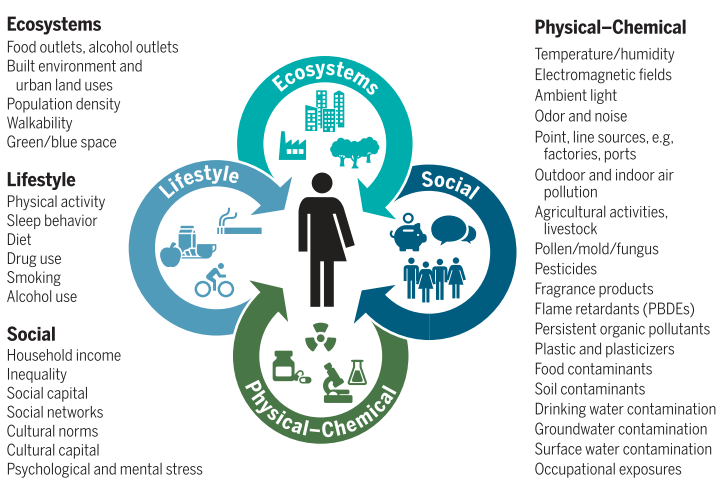
\includegraphics{images/exposome.png}
\caption{The exposome (figure from Vermeulen et al.~2020)}
\end{figure}

Even restricting our interest to environmental exposures, a substantial component of the exposome, it is recognized that we are simultaneously exposed to hundreds of chemicals and pollutants, and it has been shown that a given blood or urine sample taken from a random American will contain some concentration of at least 400 different chemicals. A group of 3 or more chemicals/pollutants, simultaneously present in nature or in the human body, is commonly defined as an environmental mixture.

\hypertarget{why-focusing-on-multiple-exposures}{%
\section{Why focusing on multiple exposures?}\label{why-focusing-on-multiple-exposures}}

Common approaches that have been used on a daily basis in environmental epidemiology might fail to capture the complexity of exposures in our world. For several years, despite recognizing that individuals are generaly exposed to multiple environmental factors, the ``one-at-the-time'' approach has remained the standard practice in most epidemiological research. To better understand what we mean by ``one-at-the-time'' approach, and its limitations, let's think of a study where we want to evaluate the effects of parabens - endocrine disrupting chemicals commonly used in the production of personal care products and cosmetics - on diabetes in a population of 1000 individuals. Let's assume that through urine samples analysis we were able to detect concentrations of three common parabens compounds (metylparaben, butylparaben, propylparaben) in most of our individuals. The ``one-at-the-time'' approach would build 3 independent statistical models (these could even be very sophisticated models that account for any level of data complexity), one for each parabens compound, adjusting for potential confounders of the associations but without taking into account the other 2 detected compounds. When this approach is chosen we encounter three main limiations:

\begin{itemize}
\item
  We know that individuals are exposed to multiple factors, and we might want to estimate the joint (also knows as cumulative) effects of these chemicals. A ``one-at-the-time'' approach does not allow responding to this question.
\item
  Is there any interaction between the three compounds in predicting diabetes? A ``one-at-the-time'' approach does not allow responding to this question.
\item
  Last but not least, this approach is making strong assumptions with regards to the causal structure underlying the data. Specifically, we are assuming that, very unrealistically, the association between each compound and the outcome is not confounded by the presence of any of the other compounds.
\end{itemize}

To overcome these 3 major limitations we need to evaluate exposure to parabens as a mixture of the three evaluated compounds, building a single statistical model that could jointly evaluate the three exposures and possibly accounting for co-confounding, interactions, and other specific features of the data. Obtaining such statistical model is not easy, and things would only get more complex if we wanted to account for a larger mixture of chemicals, or even to incorporate several groups of exposures in an exposome-wide analysis. Over the last decade or so, many researchers have focused their effort on developing statistical approaches for environmental mixtures, adapting techniques from other fields or developing new methodologies from scratch. The National Institute of Environmental Health Sciences (NIEHS) launched a specific initiative, called Powering Research Through Innovative Methods for Mixtures in Epidemiology (PRIME), to encourage methods developments in this direction, and organized workshops and symposiums on the topics. An important symposium in 2015 identified several available approaches and discussed advantages and limitations for each \citep{taylor2016statistical}.

\begin{figure}
\centering
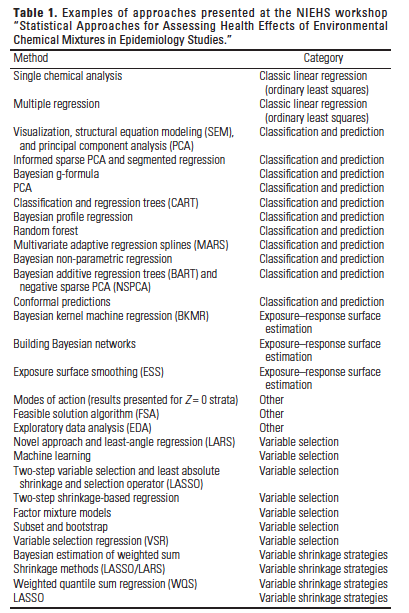
\includegraphics{images/table.png}
\caption{Approaches discussed by NIEHS in 2015 (from Taylor et al.~2016)}
\end{figure}

Five years later the number of available approaches has multiplied, and several of the discussed methodologies has been extended, revised, and presented to the public. The field of environmental epidemiology is gradually moving to a multi-pollutants or multi-chemical framework as a default \citep{dominici2010protecting}, leading the ground in exposome research, and more and more papers are published within this topic.

The goal of this class is to present and discuss some of these approaches, presenting their advantages and limitations and, most importantly, discussing what research question they target and when they should be chosen to evaluate environmental mixtures. While it is impossible to cover all available techniques, we will provide a set of references for alternative methodologies that are not discussed here. Finally, most of the examples and discussion will focus on environmental exposures. It comes without saying that extension of these approaches into other fields of exposome research (e.g.~evaluating multiple nutrients, multiple lifestyle factors \dots) is recommended and would provide enormous benefits.

\hypertarget{what-is-your-research-question}{%
\section{What is your research question?}\label{what-is-your-research-question}}

When evaluating a set of environmental factors detected in a given population as an environmental mixture, a critical step is the identification of the research question of interest. The discussion of the different methodologies presented in the aforementioned NIEHS workshop concluded that we do not have an optimal approach, but that each method performed well under a specific research question. Here are some of the most common questions that we may want to address:

\begin{enumerate}
\def\labelenumi{\arabic{enumi}.}
\tightlist
\item
  Do we have recurrent patterns of exposures?
\end{enumerate}

With several factors at play, it is often of interest to understand whether specific components of the mixture are clustered into smaller subgroups, based on similar characteristics, shared sources, or other features.

\begin{enumerate}
\def\labelenumi{\arabic{enumi}.}
\setcounter{enumi}{1}
\tightlist
\item
  What is the overall effect of the mixture on a given outcome?
\end{enumerate}

From our previous example, we may be interested in evaluating the overall effects of parabens exposure on the risk of diabetes. We are not really interested in the specific role of each compound but only on the cumulative effect of the several components.

\begin{enumerate}
\def\labelenumi{\arabic{enumi}.}
\setcounter{enumi}{2}
\tightlist
\item
  Who are the bad actors? What are the individual effects within the mixture?
\end{enumerate}

Let's assume that we have identified a potentially harmful effect of our mixture on the outcome of interest, and therefore we want to reduce the levels of exposures in our population. If question 1 has identified common patterns due to shared sources, we could simply target these sources, disregarding the actual effects of these chemicals. Alternatively, we could try to identify which component of the mixture is responsible for the effect observed in question 2. In our parabens example, if we had observed a positive association we may want to further investigate whether it is MP, PP, BP, or more than one of them, driving the association between the mixture and the outcome.

\begin{enumerate}
\def\labelenumi{\arabic{enumi}.}
\setcounter{enumi}{3}
\tightlist
\item
  Is there any interaction between chemicals in predicting the outcome?
\end{enumerate}

When more than one mixture component contributes to a given mixture-outcome association, it is reasonable to expect that some kind of interaction between the 2 will be present.

In general, one might have one or more research questions in mind, or simply want to evaluate the mixture in an exploratory way. No matter what, it will always be recommended to explore different techniques and thoroughly compare and validate results.

\hypertarget{broad-classifications-of-statistical-approaches}{%
\section{Broad classification(s) of statistical approaches}\label{broad-classifications-of-statistical-approaches}}

Over the last few years several papers have reviewed the existing literature on statistical methods for mixtures and provide different criteria for their classifications \citep{hamra2018environmental}, \citep{stafoggia2017statistical}. Simple and relevant classification criteria are the following:

\begin{enumerate}
\def\labelenumi{\arabic{enumi}.}
\tightlist
\item
  Supervised vs unsupervised procedures
\end{enumerate}

This first distinction refers to whether or not the mixture is evaluated by taking into account its association with a given outcome of interest. We will see in Section 2 that, before evaluating the effects of our exposures on health outcomes, it is important to carefully assess the structure of the mixture, especially when this is composed by several components, investigating its correlations structure and identifying the presence of subgroups or clusters of exposures. To this end, unsupervised techniques directly focus on characterizing the complex mixture of exposures without any reference to a given outcome of interest. Supervised techniques, on the other hand, attempt to account for the complex nature of exposures while investigating a given mixture-outcome association.

\begin{enumerate}
\def\labelenumi{\arabic{enumi}.}
\setcounter{enumi}{1}
\tightlist
\item
  Data reduction vs variable selection techniques.
\end{enumerate}

The goal of all techniques we will cover is to reduce the complexity of the data to be able to assess mixtures-outcome associations, while maintaining as much information as possible. This is broadly done in two way: by summarizing the original exposures into fewer and easier to deal with covariates, or by selecting targeted elements of the mixture. We can use the term ``data reduction approaches'' to describe those techniques that reduce the dimension of the mixture by generating new variables (scores, components, indexes \dots). On the other hand, ``variable selection approaches'' are those that select specific elements of the mixture that are directly evaluated with respect to the outcome.

\hypertarget{introduction-to-r-and-the-simulated-data}{%
\section{Introduction to R and the simulated data}\label{introduction-to-r-and-the-simulated-data}}

All methods that we will present can be used in the R statistical software. An introduction to R, for those unfamiliar with the software, can be found here: \url{https://rpubs.com/alecri/intro-epiR}. R is a free statistical software environment that allows you to write your own code and packages, sharing them as open sources. For this reason, it is common that any newly developed statistical method will first be implemented in R. As such, several recently developed approaches for environmental mixtures are only available in R. Most R packages are accompanied by online tutorials and vignettes that describe all features of the library and provide illustrative examples and explanations. We refer to those documents for the technical information of the R packages, and only focus here on methods implementation and results interpretation. The following packages will be used:

\begin{Shaded}
\begin{Highlighting}[]
\NormalTok{Packages }\OtherTok{\textless{}{-}} \FunctionTok{c}\NormalTok{(}\StringTok{"readxl"}\NormalTok{, }\StringTok{"bkmr"}\NormalTok{, }\StringTok{"qgraph"}\NormalTok{, }\StringTok{"gWQS"}\NormalTok{, }\StringTok{"qgcomp"}\NormalTok{, }\StringTok{"corrplot"}\NormalTok{, }\StringTok{"cluster"}\NormalTok{,}\StringTok{"factoextra"}\NormalTok{,}\StringTok{"gridExtra"}\NormalTok{,}\StringTok{"table1"}\NormalTok{,}\StringTok{"glmnet"}\NormalTok{)}
\FunctionTok{lapply}\NormalTok{(Packages, library, }\AttributeTok{character.only =} \ConstantTok{TRUE}\NormalTok{)}
\end{Highlighting}
\end{Shaded}

As an illustrative example we will use a simulated dataset that was developed for the 2015 NIEHS workshop previously mentioned and made publicly available. The dataset is available here (under Data Set \#2 \url{https://www.niehs.nih.gov/news/events/pastmtg/2015/statistical/index.cfm}) and a description of the data structure is also provided. Specifically, the data includes a mixture of 14 continuous exposures, (\(X_1-X_{14}\)), a continuous outcome \(Y\), and 3 additional covariates (\(Z_1-Z_3\)).

\begin{table}

\caption{\label{tab:unnamed-chunk-3}First rows of the dataset}
\centering
\begin{tabular}[t]{r|r|r|r|r|r|r|r|r|r|r|r|r|r|r|r|r|r|r}
\hline
Obs & y & x1 & x2 & x3 & x4 & x5 & x6 & x7 & x8 & x9 & x10 & x11 & x12 & x13 & x14 & z1 & z2 & z3\\
\hline
1 & 3.35244 & 0.48719 & -2.81309 & -0.15955 & 0.95293 & -0.83727 & -0.00003 & 0.97400 & 2.13765 & 1.39604 & 3.56099 & 4.26839 & 0.45545 & 0.72929 & 0.57650 & 0.98552 & 8.695 & 0\\
\hline
2 & 3.69033 & 0.82919 & -2.55938 & 2.68266 & 3.77467 & 1.81320 & 1.91995 & 1.18520 & 2.66005 & 0.96977 & 2.71796 & 4.95887 & 0.60921 & 0.52988 & 1.96180 & 3.71546 & 43.606 & 0\\
\hline
3 & 3.57359 & 0.95442 & -1.68660 & 0.90617 & 1.53099 & -0.52228 & 0.66634 & 0.91016 & 2.79356 & 1.77319 & 3.60018 & 6.34345 & 0.52247 & 0.28810 & 1.51987 & -0.26049 & 35.179 & 0\\
\hline
4 & 4.08506 & 0.44262 & -2.32889 & 2.87066 & 3.69266 & 2.23544 & 0.96392 & 0.45412 & 4.38613 & 0.45019 & 3.39090 & 5.23588 & -0.13227 & -0.15786 & 1.29478 & 3.50177 & 53.850 & 0\\
\hline
5 & 4.32196 & 0.90320 & -2.64624 & 1.85611 & 2.66537 & 0.66575 & 1.22047 & 2.13394 & 3.25436 & 1.68486 & 3.35262 & 5.76463 & 0.71263 & 0.86847 & 1.49974 & 2.48495 & 46.692 & 0\\
\hline
6 & 4.48195 & 2.19892 & -2.82971 & 2.77514 & 3.93696 & 1.15633 & 1.15479 & 1.33877 & 1.65140 & 1.21884 & 2.65061 & 5.38122 & 0.46648 & 0.45505 & 1.09930 & 3.25059 & 33.677 & 0\\
\hline
\end{tabular}
\end{table}

By actually knowing the actual associations we will be able to evaluate how well each method performs with respect to the several research questions of interest. Specifically, chemical concentrations were generated based on the correlation between log-transformed PCBs, dioxins, and furans, from NHANES data. Two clusters of highly-correlated covariates were present (\(X_3-X_4-X_5\), and \(X_{12}- X_{13}\), while low to moderate correlations were simulated between other covariates. \(Z_1\) and \(Z_2\) were simulated based on poverty index and age, both assumed to be confounders of the association. \(Z_3\) was simulated based on gender distribution, and assumed to be an effect modifier. The outcome was generated with the following functions for male and female, respectively:

\[Z_3=0: E[Y]=3 + 0.05*X_4 + 0.1*X_6 + 0.1*X_{11} + 0.5*X_{12} + 0.1*X_{14} + 0.01*Z_1 + 0.003*Z_2  \]
\[Z_3=1: E[Y]=3 + 0.01*X_1 + 0.05*X_4 + 0.1*X_{11} + 0.1*X_{14} + 0.01*Z_1 + 0.003*Z_2 – 0.32*(Z_3=1) \]

Thus, for \(Z_3=0\) only \(X_4, X_6, X_{11}, X_{12}\) and \(X_{14}\) are positively associated with \(Y\). When \(Z_3=1\), only \(X_1, X_4, X_{11}\) and \(X_{14}\) are associated with \(Y\). Interactions between chemicals were not considered.

\hypertarget{unsupervised-analysis}{%
\chapter{Unsupervised analysis}\label{unsupervised-analysis}}

As introduced in the previous section, the term unsupervised analysis refers to that critical part of the analytic phase where we only focus on the exposures, trying to characterize, explain, and describe the complex environmental mixture of interest. This could even be the ultimate goal of the analysis (as a matter of fact, to respond to common questions such as ``what are the most common exposures in our populations?'' or ``can we identify subgroups of exposures that are often found together?'' we do not to account for the outcome. In other setting, this will be an important part that will inform subsequent analytic steps.

Note that here the focus is not on understanding biological mechanisms through which chemicals or pollutants operate in the body. The focus on unsupervised analysis in this context is, instead, a descriptive and epidemiologic one. When we are attempting to identify clusters of exposures without accounting the their relationship with a given outcome, the grouping will be based on aspects such as population distribution and shared sources rather than on similar mechanisms of action.

\hypertarget{pre-processing}{%
\section{Pre-processing}\label{pre-processing}}

Before getting into the actual analysis of the mixture it is important to carefully assess each component independently. Environmental exposures such as chemicals or pollutants, but also indicators of greenness, noise, or temperature, share important characteristics that complicate their statistical evaluation.

\begin{itemize}
\item
  Skewedness and variance. Exposures are often non-negative and heavily skewed on the right due to the presence of outliers and to the fact that they are strictly non-negative. For this reason, it is usually recommended to log-transform these exposures. Nevertheless, when such operation is taken into account, researchers have to deal with decisions on how to treat eventual zero-values that do not necessarily represent missing data.
\item
  Centering and standardizing exposures. Mixture components tend to have different and difficult to compare measurements and variability, even within the same family of exposures. Since these exposures will be eventually evaluated together, centering and standardizing the covariates will allow comparability and better interpretation of statistical findings.
\item
  Zero values. It is relatively common, when evaluating large mixtures of environmental exposures, to encounter one or more covariates with a considerable amount of values equal to 0. How to deal with such zero-values will have important consequences on the implementation and interpretation of statistical approaches for mixtures. The first question to consider is what these zero values represent: specifically, are they ``real zeros'' (i.e.~the individuals had no exposure to a given chemical), or do they represent non-detected values (i.e.~the individual had a low level of exposure that we were not able to detect)? In the first case, the values will have to be treated as an actual zero, with important implications for the analysis (we will briefly deal with this when talking about zero-inflated covariates in Section 6). In the second case, non-detected values are usually imputed to a predefined value (several approaches are available) and the covariate can be treated as continuous.
\item
  Missing values. Finally, it is important to evaluate the percentage of missing values for each exposure in our mixture. Most techniques that allow evaluating the joint effect of several covariates, including regresison models, will require a complete-case analysis. As such, an individual with just one missing values in one of the several mixture components, will be excluded from the whole analyses. If the proportion of missingness is not too high (10-15\%), multiple imputation techniques can be used, even though the user should be aware that most advanced methodologies might not be fully integrated withing a multiple implementation procedure. If the percentage of missingness is too high, there is not too much to be done, and we will have to decide whether to give up the covariate (excluding it from the mixture), or reduce the sample size (excluding all individual with missing values on that component)
\end{itemize}

The dataset we are using in our illustrative example includes simulated covariates where this pre-processing steps have been done ( all values are greater than 0, no missing data are present, covariates are log-transofmred and standardized).

\begin{figure}[H]

{\centering 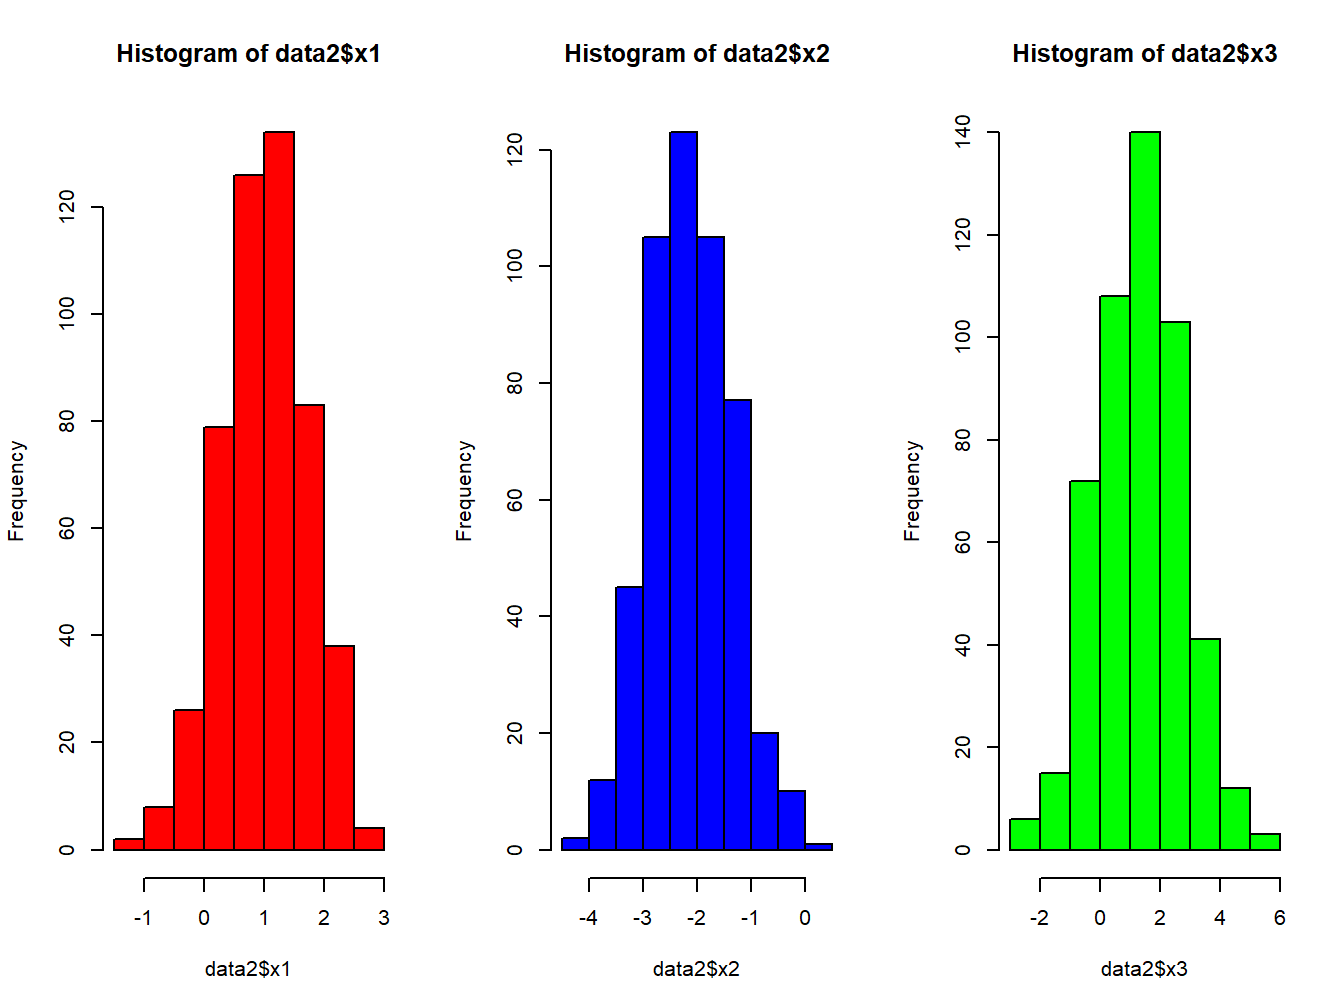
\includegraphics[width=0.8\linewidth]{bookdown-demo_files/figure-latex/figure1-1} 

}

\caption{Histogram of first 3 components}\label{fig:figure1}
\end{figure}

To conduct a thorough exploratory analysis of environmental mixtures, especially when several covariates are of interest, we encourage the use of the R package \texttt{rexposome} , fully described \href{https://www.bioconductor.org/packages/release/bioc/vignettes/rexposome/inst/doc/exposome_data_analysis.html\#multivariate-exposome-analysis}{here}

\hypertarget{correlation-analysis}{%
\section{Correlation analysis}\label{correlation-analysis}}

An essential step when evaluating an environmental mixture is the assessment of the correlation between the mixture components. This preliminary analysis gives a sense of the relationship between exposures, allows a preliminary assessment of exposures patterns and clusters, and gives important information that will suggest which method could be better suited for future modeling.

Given 2 continuous covariates, a simple assessment of their relationship can be checked with a simple two-ways scatterplots. Here we show a set of three 2x2 comparison, also adding a lowess trend line on top of the scatter plot.

\begin{figure}[H]

{\centering 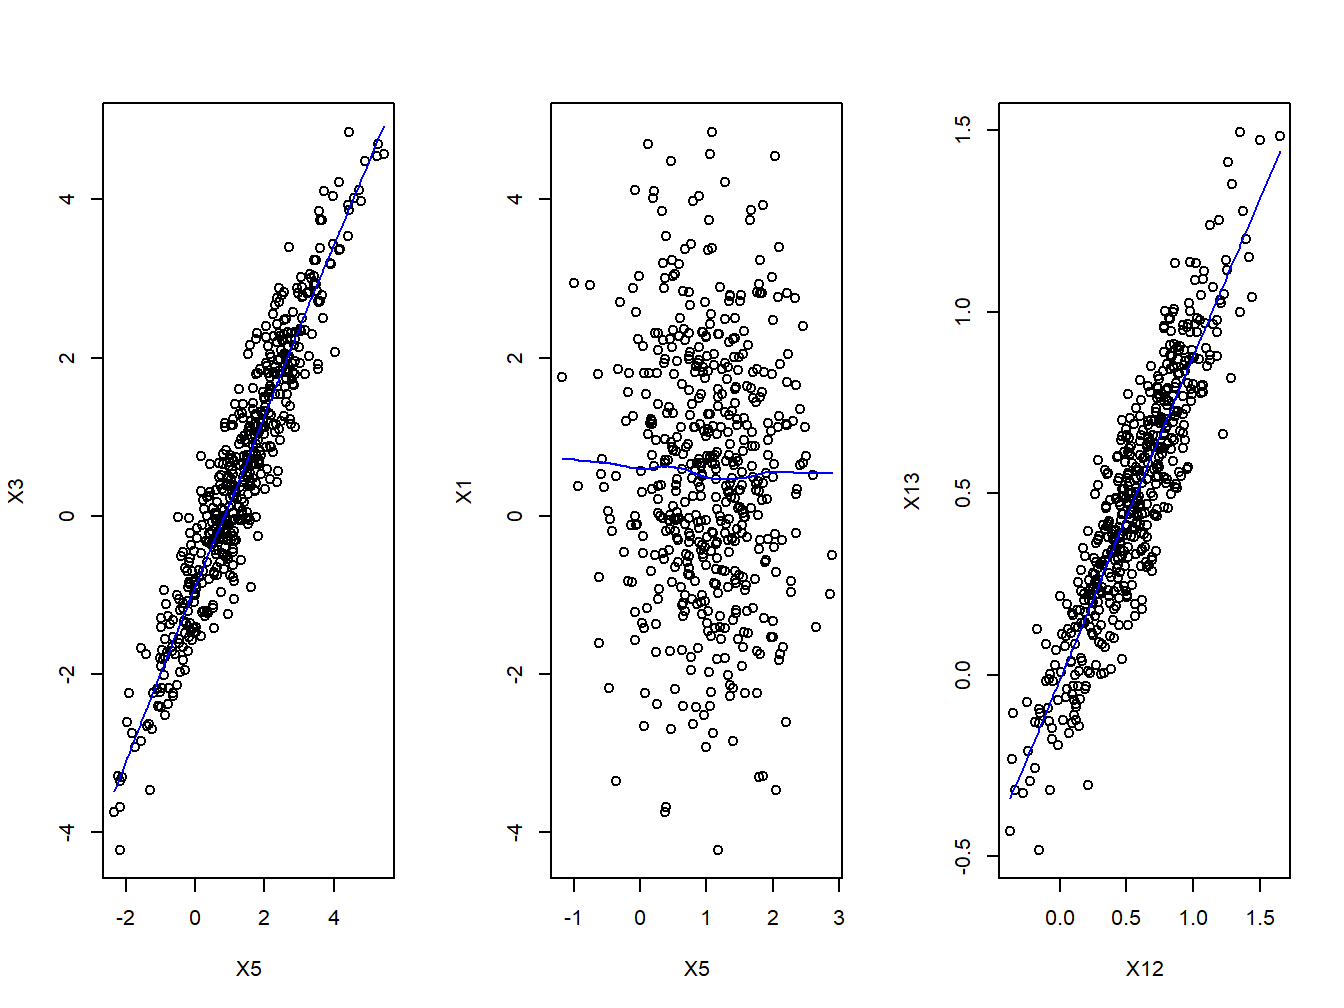
\includegraphics[width=0.8\linewidth]{bookdown-demo_files/figure-latex/figure2-1} 

}

\caption{Scatter plots}\label{fig:figure2}
\end{figure}

We see some combinations of covariates being highly correlated (like \(X_3\) and \(X_4\)), while other exposures seem to be completely independent (e.g.~\(X_1\) and \(X_5\)).

A correlation coefficient and a correlation test, will additionally provide a quantitative measure of this relationship. The Pearson correlation (\(r\)) measures the linear dependence between two variables and it can only be used when both covariates are normally distributed

\[r=\frac{\sum(x-m_x)(y-m_y)}{\sqrt{\sum(x-m_x)^2(y-m_y)^2}}\]

where \(m_x\) and \(m_y\) are the means of the two covariates \(x\) and \(y\)

The Spearman correlation (\(\rho\)) measure computes the correlation between the rank of the two covariates \(x\) and \(y\)

\[\rho=\frac{\sum(x'-m_{x'})(y'-m_{y'})}{\sqrt{\sum(x'-m_{x'})^2(y'-m_{y'})^2}}\]

where \(m_{x'}\) and \(m_{y'}\) are the ranks of \(x\) and \(y\). This correlation test is non-parametric and does not require assuming normality for the two evaluated covariates.

Both \(r\) and \(\rho\) are bounded between -1 and 1 (negative and positive correlation). There is no correlation between the covariates when the coefficient is equal to 0. Tests for significance of the correlation coefficient are available for both \(r\) and \(\rho\), testing the null hypothesis of no correlation

Here we calculate the correlation coefficients, and test, for some pair of exposures in our mixture:

\begin{Shaded}
\begin{Highlighting}[]
\NormalTok{r15 }\OtherTok{\textless{}{-}} \FunctionTok{cor.test}\NormalTok{(data2}\SpecialCharTok{$}\NormalTok{x1, data2}\SpecialCharTok{$}\NormalTok{x5, }\AttributeTok{method =} \StringTok{"pearson"}\NormalTok{)}
\NormalTok{r15}
\end{Highlighting}
\end{Shaded}

\begin{verbatim}
## 
##  Pearson's product-moment correlation
## 
## data:  data2$x1 and data2$x5
## t = -0.78615, df = 498, p-value = 0.4322
## alternative hypothesis: true correlation is not equal to 0
## 95 percent confidence interval:
##  -0.12251881  0.05264665
## sample estimates:
##         cor 
## -0.03520647
\end{verbatim}

\begin{Shaded}
\begin{Highlighting}[]
\NormalTok{rho15 }\OtherTok{\textless{}{-}} \FunctionTok{cor.test}\NormalTok{(data2}\SpecialCharTok{$}\NormalTok{x1, data2}\SpecialCharTok{$}\NormalTok{x5, }\AttributeTok{method =} \StringTok{"spearman"}\NormalTok{)}
\NormalTok{rho15}
\end{Highlighting}
\end{Shaded}

\begin{verbatim}
## 
##  Spearman's rank correlation rho
## 
## data:  data2$x1 and data2$x5
## S = 21488934, p-value = 0.4824
## alternative hypothesis: true rho is not equal to 0
## sample estimates:
##         rho 
## -0.03147296
\end{verbatim}

\begin{Shaded}
\begin{Highlighting}[]
\NormalTok{r1213 }\OtherTok{\textless{}{-}} \FunctionTok{cor.test}\NormalTok{(data2}\SpecialCharTok{$}\NormalTok{x12, data2}\SpecialCharTok{$}\NormalTok{x13, }\AttributeTok{method =} \StringTok{"pearson"}\NormalTok{)}
\NormalTok{r1213}
\end{Highlighting}
\end{Shaded}

\begin{verbatim}
## 
##  Pearson's product-moment correlation
## 
## data:  data2$x12 and data2$x13
## t = 47.687, df = 498, p-value < 2.2e-16
## alternative hypothesis: true correlation is not equal to 0
## 95 percent confidence interval:
##  0.8886169 0.9203247
## sample estimates:
##     cor 
## 0.90573
\end{verbatim}

\begin{Shaded}
\begin{Highlighting}[]
\NormalTok{rho1213 }\OtherTok{\textless{}{-}} \FunctionTok{cor.test}\NormalTok{(data2}\SpecialCharTok{$}\NormalTok{x12, data2}\SpecialCharTok{$}\NormalTok{x13, }\AttributeTok{method =} \StringTok{"spearman"}\NormalTok{)}
\NormalTok{rho1213}
\end{Highlighting}
\end{Shaded}

\begin{verbatim}
## 
##  Spearman's rank correlation rho
## 
## data:  data2$x12 and data2$x13
## S = 2113532, p-value < 2.2e-16
## alternative hypothesis: true rho is not equal to 0
## sample estimates:
##       rho 
## 0.8985501
\end{verbatim}

When evaluating the correlation between several exposures we can create a correlation matrix

\begin{Shaded}
\begin{Highlighting}[]
\CommentTok{\#Correlation matrix}
\NormalTok{cor.matrix }\OtherTok{\textless{}{-}} \FunctionTok{cor}\NormalTok{ (data2[,}\DecValTok{3}\SpecialCharTok{:}\DecValTok{16}\NormalTok{], }\AttributeTok{method =} \StringTok{"spearman"}\NormalTok{)}
\NormalTok{knitr}\SpecialCharTok{::}\FunctionTok{kable}\NormalTok{(}
\NormalTok{  cor.matrix, }\AttributeTok{booktabs =} \ConstantTok{TRUE}\NormalTok{,}
  \AttributeTok{caption =} \StringTok{\textquotesingle{}Correlation matrix\textquotesingle{}}
\NormalTok{)}
\end{Highlighting}
\end{Shaded}

\begin{table}

\caption{\label{tab:unnamed-chunk-6}Correlation matrix}
\centering
\begin{tabular}[t]{lrrrrrrrrrrrrrr}
\toprule
  & x1 & x2 & x3 & x4 & x5 & x6 & x7 & x8 & x9 & x10 & x11 & x12 & x13 & x14\\
\midrule
x1 & 1.0000000 & 0.3015516 & -0.0443238 & -0.0277916 & -0.0314730 & 0.0355735 & 0.1636032 & -0.0453658 & 0.1525454 & -0.1027089 & -0.1102655 & 0.3459623 & 0.3358113 & 0.0099408\\
x2 & 0.3015516 & 1.0000000 & 0.0525986 & 0.0624227 & 0.0846338 & 0.0693562 & 0.1827964 & 0.0299643 & 0.1357383 & -0.0186805 & -0.0251231 & 0.3923731 & 0.3821572 & 0.0482436\\
x3 & -0.0443238 & 0.0525986 & 1.0000000 & 0.9874641 & 0.9326813 & 0.5992095 & 0.2848127 & 0.7373648 & 0.1720033 & 0.4028520 & 0.5609233 & -0.1051226 & -0.1411885 & 0.7041847\\
x4 & -0.0277916 & 0.0624227 & 0.9874641 & 1.0000000 & 0.9410680 & 0.6075068 & 0.2893180 & 0.7419298 & 0.1757588 & 0.4087219 & 0.5662499 & -0.0938162 & -0.1289154 & 0.7113510\\
x5 & -0.0314730 & 0.0846338 & 0.9326813 & 0.9410680 & 1.0000000 & 0.5931920 & 0.2946356 & 0.7244964 & 0.1676753 & 0.4165967 & 0.5632797 & -0.1040214 & -0.1430413 & 0.6895982\\
\addlinespace
x6 & 0.0355735 & 0.0693562 & 0.5992095 & 0.6075068 & 0.5931920 & 1.0000000 & 0.4614976 & 0.6356481 & 0.3805305 & 0.4460931 & 0.5435489 & 0.0582305 & 0.0282746 & 0.6183391\\
x7 & 0.1636032 & 0.1827964 & 0.2848127 & 0.2893180 & 0.2946356 & 0.4614976 & 1.0000000 & 0.3906414 & 0.6974279 & 0.3637349 & 0.4113740 & 0.4586443 & 0.4831571 & 0.4081206\\
x8 & -0.0453658 & 0.0299643 & 0.7373648 & 0.7419298 & 0.7244964 & 0.6356481 & 0.3906414 & 1.0000000 & 0.3707775 & 0.5494283 & 0.6431383 & 0.0104423 & -0.0333734 & 0.7430785\\
x9 & 0.1525454 & 0.1357383 & 0.1720033 & 0.1757588 & 0.1676753 & 0.3805305 & 0.6974279 & 0.3707775 & 1.0000000 & 0.3177311 & 0.3558096 & 0.5047644 & 0.4954366 & 0.3966118\\
x10 & -0.1027089 & -0.0186805 & 0.4028520 & 0.4087219 & 0.4165967 & 0.4460931 & 0.3637349 & 0.5494283 & 0.3177311 & 1.0000000 & 0.7741935 & 0.0031582 & -0.0451602 & 0.4188343\\
\addlinespace
x11 & -0.1102655 & -0.0251231 & 0.5609233 & 0.5662499 & 0.5632797 & 0.5435489 & 0.4113740 & 0.6431383 & 0.3558096 & 0.7741935 & 1.0000000 & -0.0115591 & -0.0697092 & 0.5384582\\
x12 & 0.3459623 & 0.3923731 & -0.1051226 & -0.0938162 & -0.1040214 & 0.0582305 & 0.4586443 & 0.0104423 & 0.5047644 & 0.0031582 & -0.0115591 & 1.0000000 & 0.8985501 & 0.1073926\\
x13 & 0.3358113 & 0.3821572 & -0.1411885 & -0.1289154 & -0.1430413 & 0.0282746 & 0.4831571 & -0.0333734 & 0.4954366 & -0.0451602 & -0.0697092 & 0.8985501 & 1.0000000 & 0.0694033\\
x14 & 0.0099408 & 0.0482436 & 0.7041847 & 0.7113510 & 0.6895982 & 0.6183391 & 0.4081206 & 0.7430785 & 0.3966118 & 0.4188343 & 0.5384582 & 0.1073926 & 0.0694033 & 1.0000000\\
\bottomrule
\end{tabular}
\end{table}

While informative, this is not a really nice way of presenting results, and we prefer to use graphical tools such as the Correlation plot (or, correlogram) This is done by using the package \texttt{corrplot}. Note that the command requires you use the correlation matrix you previously defined.

\begin{Shaded}
\begin{Highlighting}[]
\FunctionTok{corrplot}\NormalTok{(cor.matrix,}
         \AttributeTok{method=}\StringTok{"circle"}\NormalTok{,}
         \AttributeTok{order =} \StringTok{"hclust"}\NormalTok{,}
         \AttributeTok{addrect =}\DecValTok{10}\NormalTok{,}
         \AttributeTok{tl.pos =} \StringTok{"l"}\NormalTok{,}
         \AttributeTok{tl.col =} \StringTok{"black"}\NormalTok{,}
         \AttributeTok{sig.level =} \FloatTok{0.05}\NormalTok{)}
\end{Highlighting}
\end{Shaded}

\begin{figure}[H]

{\centering 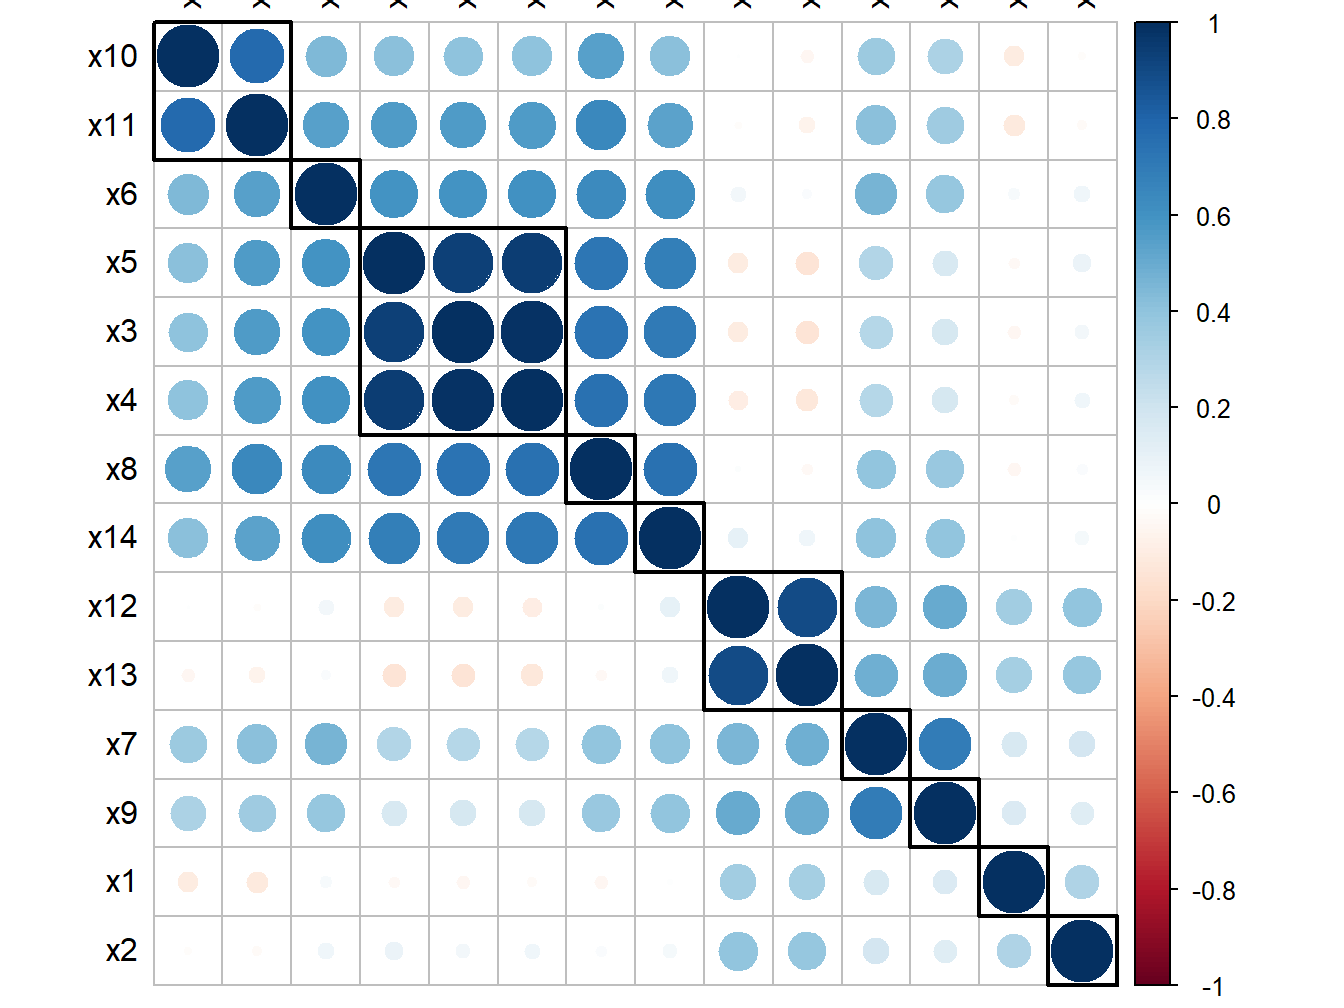
\includegraphics[width=0.8\linewidth]{bookdown-demo_files/figure-latex/figure-1} 

}

\caption{Correlation Plot}\label{fig:figure}
\end{figure}

\href{https://cran.r-project.org/web/packages/corrplot/vignettes/corrplot-intro.html}{This} link provides a very useful description of the several \texttt{corrplot} options.

The correlation plot in the example provides several important information: first of all, we see a cluster of highly correlated exposures (\(X_3\),\(X_4\),\(X_5\)), and a cluster of moderately correlated exposures (\(X_{12}\), \(X_{13}\)). In addition, we observe that low to moderate levels of correlation also exist between most pairs of exposures, and it is not straightforward to identify clearly define additional subgroups of exposures.

\hypertarget{weighted-correlation-network-analysis}{%
\section{Weighted correlation network analysis}\label{weighted-correlation-network-analysis}}

Network analysis is emerging as a flexible and powerful technique in different fields. In a nutshell, a network refers to a complex structure of variables, called nodes, and the relationships (formally called edges) between these nodes. Correlation networks define such relationships on the basis of their quantitative correlations, and are increasingly being used in biology to analyze high-dimensional data sets. Weighted correlation networks, in particular, preserve the continuous nature of the underlying correlation information without dicothomizing information. While the theory behind network analysis is beyond the scope of this course, and we refer to other publications for further details (\citet{langfelder2008wgcna}), (\citet{hevey2018network}), it is here useful to mention that these networks can be used in descriptive analyses to graphically display the relationship between exposures in our mixture based on the correlation structure. This can be now obtained with several R packages, including \texttt{qgraph}, documented \href{http://sachaepskamp.com/files/Cookbook.html\#pearson-correlations}{here}.

\begin{figure}[H]

{\centering 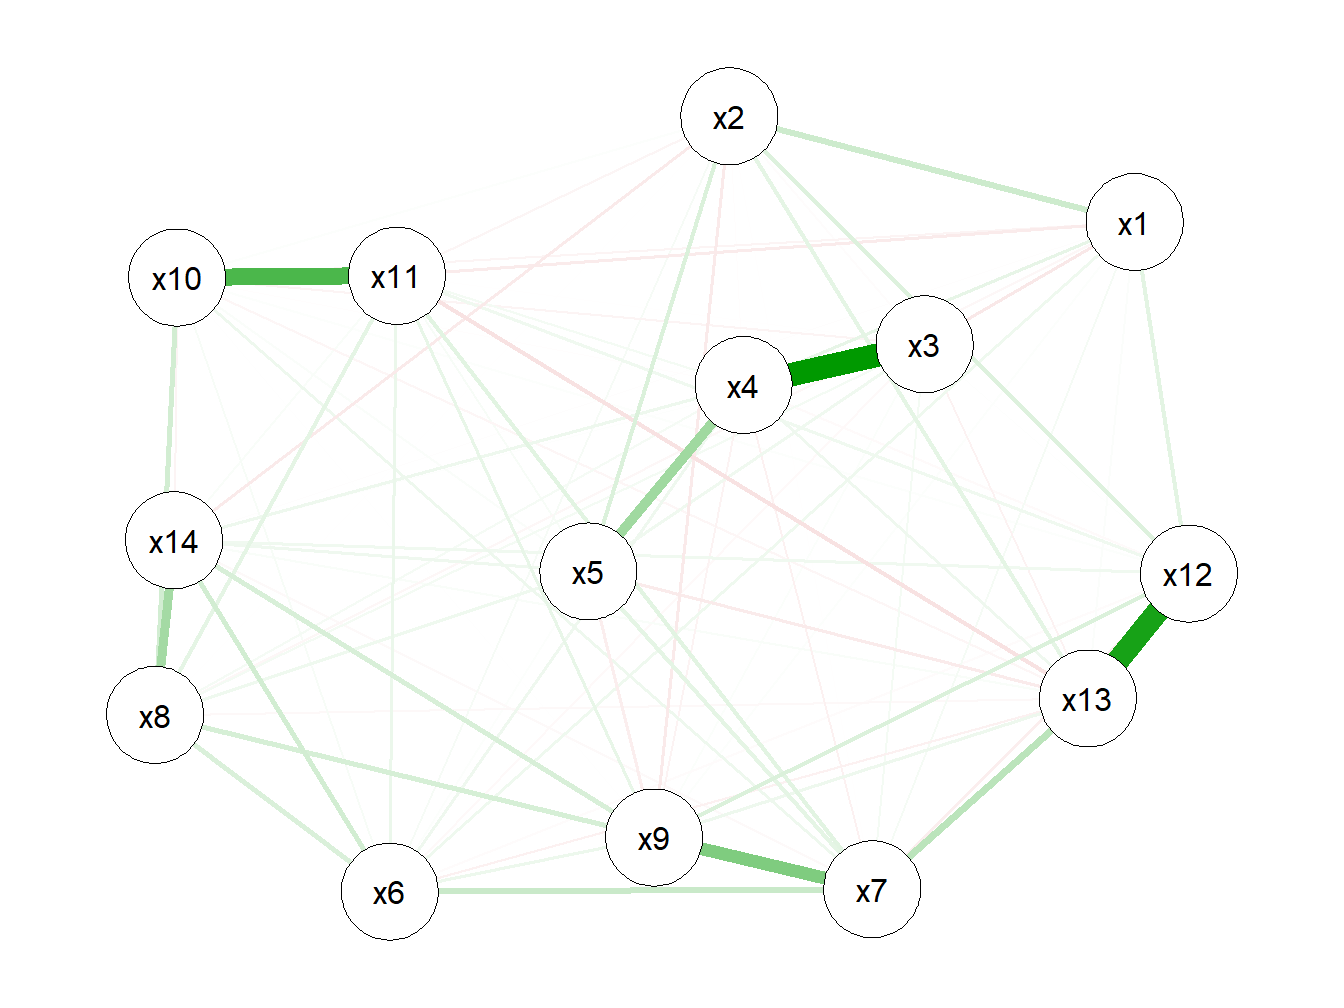
\includegraphics[width=0.8\linewidth]{bookdown-demo_files/figure-latex/figure3-1} 

}

\caption{Weighted correlation network}\label{fig:figure3}
\end{figure}

This network confirms our finding from the correlation plot, but provides a different and possibly better way of representing and visualizing the relationships between components of the mixture.

\hypertarget{principal-component-analysis}{%
\section{Principal component analysis}\label{principal-component-analysis}}

Principal Component Analysis (PCA) is a useful technique for exploratory data analysis, which allows a better visualization of the variability present in a dataset with many variables. This ``better visualization'' is achieved by transforming a set of covariates into a smaller set of Principal Components.

A principal component can be thought of as the direction where there is the most variance or, geometrically speaking, where the data is most spread out. In practical terms, to derive the first principal component that describe our mixture, we try to find the straight line that best spreads the data out when it is projected along it, thus explaining the most substantial variance in the data. The following Figure shows the first principal component in a simple setting with only 3 covariates of interest (so that we could graphically represent it):

\begin{figure}
\centering
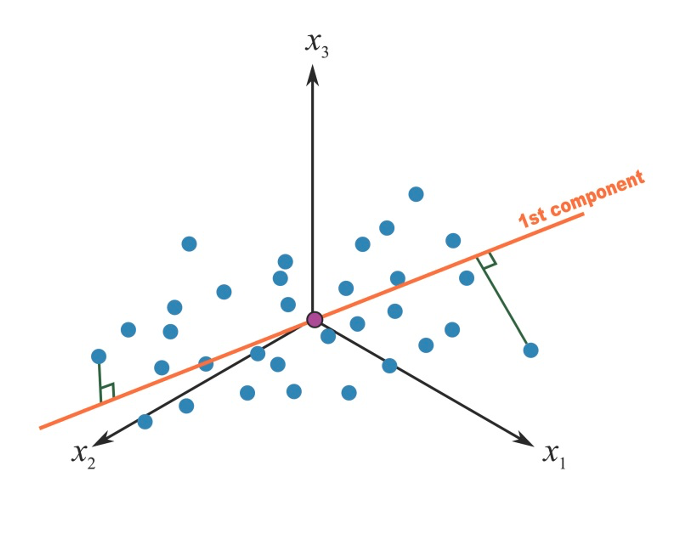
\includegraphics{images/pca1.png}
\caption{First principal component in a 3-covariates setting}
\end{figure}

Mathematically speaking, this first component \(t_1\) is calculated as a linear combination of the \(p\) original predictors \(T=XW_p\), where \(W_p\) are weights that would maximize the overall explained variability. For those math-oriented readers, it turns out that such weights are the eigenvectors of the correlation matrix of the original exposures.

Once a first component has been retrieved, we proceed by calculating a second component that would maximize the residual variance. Of interest in our context, the procedure adds a constraints of orthogonality to this second component, that is, it will be uncorrelated to the first one, as presented in the figure.

\begin{figure}
\centering
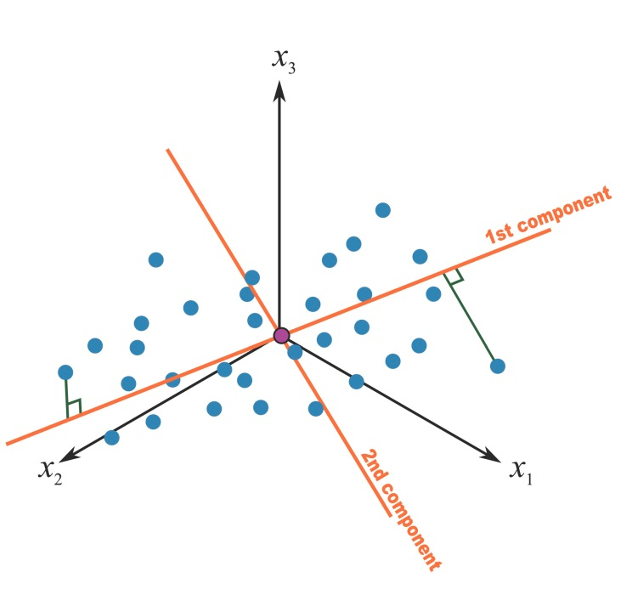
\includegraphics{images/pca2.png}
\caption{First principal component in a 3-covariates setting}
\end{figure}

Mathematically, this is obtained by another linear combination where the weights are the eigenvectors corresponding to the second largest eigenvalue. In this way we can proceed to derive a full set of \(p\) components from our original \(p\) covariates, until all variance has been explained. In summary, PCA is a set of linear transformation that fits the matrix of exposures into a new coordinate system so that the most variance is explained by the first coordinate, and each subsequent coordinate is orthogonal to the last and has a lesser variance. You transform a set of \(p\) correlated variables into a set of \(p\) uncorrelated principal components. PCA is sensitive to unscaled covariates, so it is usually recommended to standardize your matrix of exposures before running a PCA analysis.

\hypertarget{fitting-a-pca-in-r}{%
\subsection{Fitting a PCA in R}\label{fitting-a-pca-in-r}}

There are several options to conduct PCA in R. Here we will use \texttt{prcomp} but alternative options are available (\texttt{princomp} and \texttt{principal}). PCA is also available in the aforementioned \texttt{rexposome} package. If you want to prepare nice figures for presentations or usage in manuscripts, I also recommend taking a look a the \texttt{factoextra} package to create a ggplot2-based elegant visualization (\href{http://www.sthda.com/english/wiki/factoextra-r-package-easy-multivariate-data-analyses-and-elegant-visualization}{link}).

The \texttt{prcomp(\ )} function produces a basic principal component analysis. The command requires the raw data you want to reduce (the exposure matrix) and will extract principal components. Here we are also centering and scaling all exposures. Table 2.2. shows the first rows of the newly derived variables (the components).

\begin{Shaded}
\begin{Highlighting}[]
\NormalTok{fit }\OtherTok{\textless{}{-}} \FunctionTok{prcomp}\NormalTok{(X, }\AttributeTok{center=}\ConstantTok{TRUE}\NormalTok{, }\AttributeTok{scale=}\ConstantTok{TRUE}\NormalTok{)}
\end{Highlighting}
\end{Shaded}

\begin{table}

\caption{\label{tab:unnamed-chunk-8}First rows of the components}
\centering
\begin{tabular}[t]{r|r|r|r|r|r|r|r|r|r|r|r|r|r}
\hline
PC1 & PC2 & PC3 & PC4 & PC5 & PC6 & PC7 & PC8 & PC9 & PC10 & PC11 & PC12 & PC13 & PC14\\
\hline
-2.2389015 & 0.0189525 & -1.2859775 & -0.3216035 & -0.2117773 & 0.5065609 & 0.0949531 & 0.0498184 & -0.3528743 & 0.6327501 & -0.9635341 & -0.3863832 & -0.2260102 & 0.0393756\\
\hline
1.1559396 & -0.6968029 & 1.0199832 & -1.2520422 & 0.2019949 & 0.1850336 & 0.6115127 & -0.7637062 & -0.0160088 & -0.4436463 & -0.1977756 & 0.2647719 & 0.1831903 & 0.0473029\\
\hline
0.1629765 & -0.0676542 & -0.9676685 & 1.3357760 & -0.3980497 & -0.0163378 & 0.5089395 & 1.0205435 & -0.6352686 & -0.6295934 & 0.6662812 & 0.4333277 & 0.2718524 & -0.1982041\\
\hline
1.0947459 & -3.8859461 & 1.0072495 & 0.4083807 & -0.2634263 & 0.1651619 & 0.3376678 & 0.3956715 & -0.0564324 & 1.1606182 & 0.0526433 & 0.0768175 & -0.0135220 & -0.0826189\\
\hline
1.4205153 & 1.1283036 & -1.0392885 & -0.6507554 & 0.1587461 & 0.3137072 & -0.3465914 & -0.4683247 & 0.3952183 & 0.1897396 & 0.4224867 & -0.0995627 & 0.1514907 & -0.0933670\\
\hline
0.3557820 & -0.2771229 & 1.0902309 & -0.1366375 & 1.8059563 & 0.3943783 & -0.9437355 & -0.9424548 & -0.5576855 & -0.8672917 & 0.1908570 & 0.0755395 & 0.5675384 & 0.1145596\\
\hline
\end{tabular}
\end{table}

\hypertarget{choosing-the-number-of-components}{%
\subsection{Choosing the number of components}\label{choosing-the-number-of-components}}

One of the most interesting features of PCA is that, while it is possible to calculate \(p\) components from a set of \(p\) covariates, we usually need a smaller nummber to successfully describe most of the variance of the original matrix of exposures. In practical terms, not only we are reshaping the original set of exposures into uncorrelated principal components, but we are also able to reduce the dimension of the original matrix into a smaller number of variables that describe the mixture. How many components do we actually need? Before getting to describe the several tools that can guide us on this decision, it is important to stress that this step will be purely subjective. Sometimes these tools will lead to the same evident conclusion, but other times it might not be straightforward to identify a clear number of components to describe the original data. In general, the three common tools used to select a number of components include:

\begin{itemize}
\tightlist
\item
  Select components that explain at least 70 to 80\% of the original variance
\item
  Select components corresponding to eigenvalues larger than 1
\item
  Look at the point of inflation of the scree plot
\end{itemize}

Let's take a look at these approaches in our illustrative example. These are the results of the PCA that we ran with the previous R command:

\begin{Shaded}
\begin{Highlighting}[]
\FunctionTok{summary}\NormalTok{(fit)}
\end{Highlighting}
\end{Shaded}

\begin{verbatim}
## Importance of components:
##                           PC1    PC2     PC3     PC4     PC5     PC6     PC7
## Standard deviation     2.4627 1.7521 1.12071 0.89784 0.83905 0.72337 0.63861
## Proportion of Variance 0.4332 0.2193 0.08971 0.05758 0.05029 0.03738 0.02913
## Cumulative Proportion  0.4332 0.6525 0.74219 0.79977 0.85006 0.88744 0.91657
##                            PC8    PC9    PC10    PC11    PC12    PC13    PC14
## Standard deviation     0.60268 0.4892 0.46054 0.43573 0.29751 0.25542 0.09904
## Proportion of Variance 0.02594 0.0171 0.01515 0.01356 0.00632 0.00466 0.00070
## Cumulative Proportion  0.94251 0.9596 0.97476 0.98832 0.99464 0.99930 1.00000
\end{verbatim}

(Square roots of) eigenvalues are reported in the first line, while the second and third line present, respectively, the proportion of variance explained by each given component (note that, as expected, this decreases as we proceed with the estimation), and the cumulative variance explained.

The scree plot is the plot of the descending eigenvalues. Ideally we would like to identify a point of inflation (also known as ``elbow'' of the curve), signifying that after a certain number of components, the proportion of variance that is additionally explained becomes minimal.

\begin{Shaded}
\begin{Highlighting}[]
\FunctionTok{plot}\NormalTok{(fit,}\AttributeTok{type=}\StringTok{"lines"}\NormalTok{)}
\end{Highlighting}
\end{Shaded}

\begin{figure}
\centering
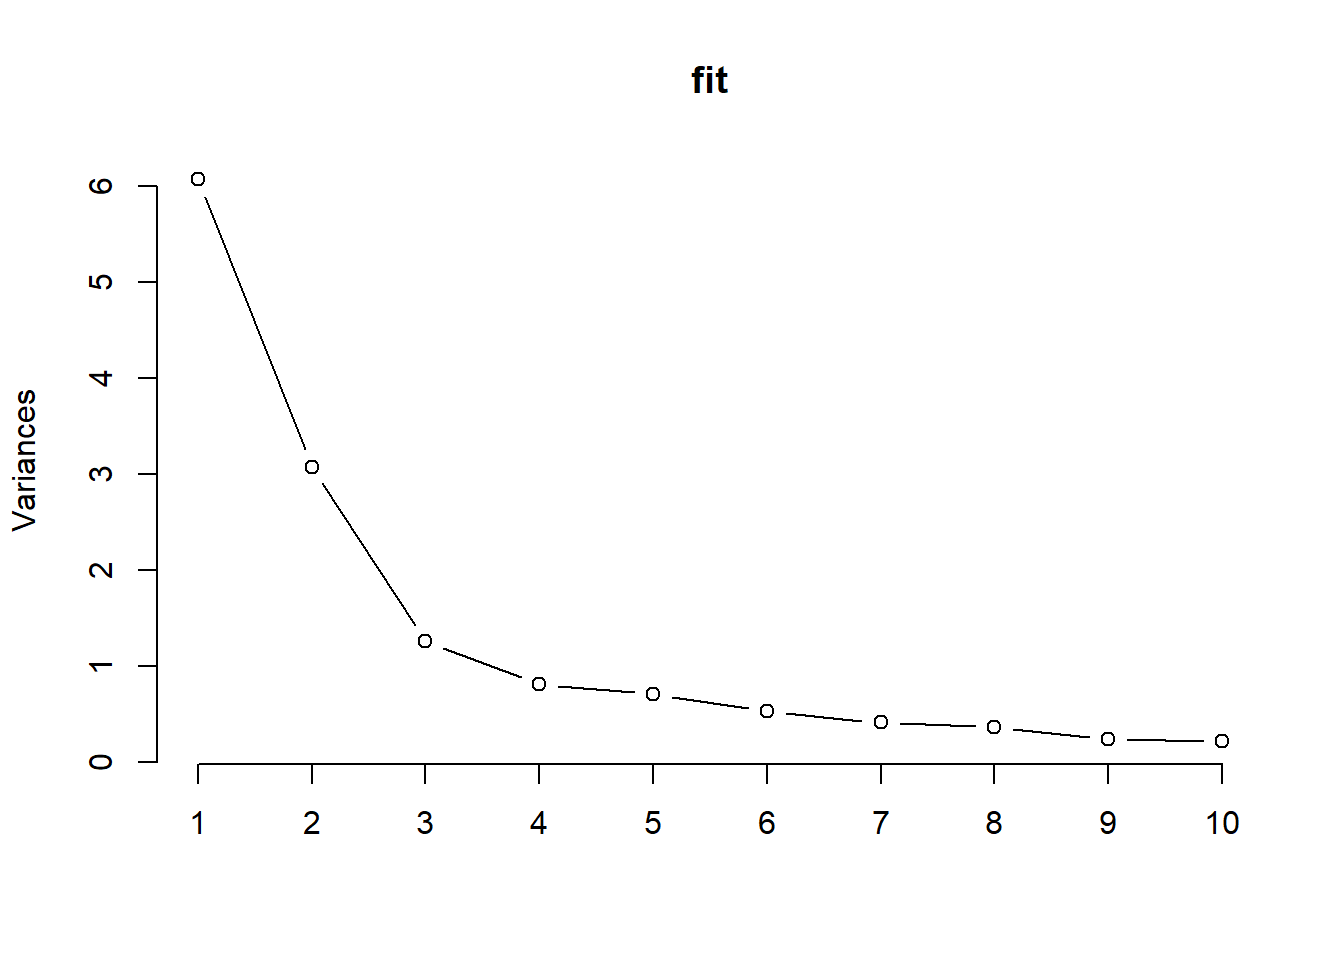
\includegraphics{bookdown-demo_files/figure-latex/screeplot-1.pdf}
\caption{\label{fig:screeplot}Scree plot}
\end{figure}

All these techniques seem to indicate that 3 components might successfully describe the original set of 14 exposures.

\hypertarget{getting-sense-of-components-interpretation}{%
\subsection{Getting sense of components interpretation}\label{getting-sense-of-components-interpretation}}

A PCA is made by three steps. Fitting the model is the easiest part as it only requires a line of coding (assuming that the pre-processing has been carefully conducted). The second step, selecting the number of components, requires some levels of subjectivity but is also relatively simple in most settings. The third step is usually the more complicated ones, as we are now tasked with providing some interpretation to the set of principal components that we have selected. To get a sense of what principal components represent, we usually look at loading factors, the correlation coefficients between the derived components and the original covariates. In practical terms they inform us on how much of the original variance of each covariate is explained by each component. Here are the loading factors for our example:

\begin{Shaded}
\begin{Highlighting}[]
\CommentTok{\#Correlation matrix}
\NormalTok{knitr}\SpecialCharTok{::}\FunctionTok{kable}\NormalTok{(}
\NormalTok{  fit}\SpecialCharTok{$}\NormalTok{rotation, }\AttributeTok{booktabs =} \ConstantTok{TRUE}\NormalTok{,}
  \AttributeTok{caption =} \StringTok{\textquotesingle{}Loading factors\textquotesingle{}}
\NormalTok{)}
\end{Highlighting}
\end{Shaded}

\begin{table}

\caption{\label{tab:unnamed-chunk-9}Loading factors}
\centering
\begin{tabular}[t]{lrrrrrrrrrrrrrr}
\toprule
  & PC1 & PC2 & PC3 & PC4 & PC5 & PC6 & PC7 & PC8 & PC9 & PC10 & PC11 & PC12 & PC13 & PC14\\
\midrule
x1 & 0.0017143 & 0.2965204 & 0.3599497 & 0.4250816 & 0.7716378 & 0.0241569 & -0.0616770 & 0.0387385 & 0.0109328 & -0.0093448 & 0.0086599 & -0.0130703 & 0.0023798 & -0.0065664\\
x2 & 0.0348101 & 0.2789407 & 0.4678814 & 0.4540801 & -0.5779524 & -0.3462568 & -0.0266760 & 0.1950322 & 0.0333408 & -0.0376913 & 0.0035594 & -0.0102783 & 0.0235316 & 0.0015467\\
x3 & 0.3581046 & -0.1358796 & 0.2730333 & -0.1308238 & -0.0277497 & 0.1564570 & -0.2131188 & -0.0881940 & -0.1294119 & -0.0178195 & -0.0636970 & -0.0951566 & 0.4535153 & -0.6688317\\
x4 & 0.3603185 & -0.1307061 & 0.2778158 & -0.1220231 & -0.0224492 & 0.1593879 & -0.1971830 & -0.1012582 & -0.1325533 & -0.0225153 & -0.0513707 & -0.0756590 & 0.3346375 & 0.7399659\\
x5 & 0.3538227 & -0.1278570 & 0.2817634 & -0.0994146 & -0.0387517 & 0.1404008 & -0.2198003 & -0.1002304 & -0.1072366 & -0.0246148 & -0.0823058 & 0.1455071 & -0.8030483 & -0.0683894\\
\addlinespace
x6 & 0.3149583 & 0.0061111 & -0.0271741 & -0.0576998 & 0.1244917 & -0.6198890 & 0.4398883 & -0.5028593 & -0.2167525 & -0.0206792 & -0.0551119 & -0.0059773 & -0.0017058 & -0.0090137\\
x7 & 0.2351557 & 0.3255146 & -0.2369090 & -0.1356534 & 0.0298706 & -0.2785907 & -0.5252466 & -0.1919585 & 0.5956024 & 0.0534903 & 0.0214018 & 0.1151769 & 0.0398633 & 0.0078041\\
x8 & 0.3589990 & -0.0482006 & -0.0071116 & -0.0053818 & 0.0322053 & 0.0151705 & 0.2523556 & 0.3158598 & 0.1335415 & 0.7818271 & 0.2730510 & -0.0112164 & -0.0151052 & -0.0010123\\
x9 & 0.1994071 & 0.3538425 & -0.3139263 & -0.1751365 & 0.0764960 & -0.2198462 & -0.2360800 & 0.5070062 & -0.5711764 & -0.0808290 & -0.0680062 & -0.0325586 & -0.0184280 & 0.0060362\\
x10 & 0.2719030 & -0.0246063 & -0.4067448 & 0.5312151 & -0.0862533 & 0.2341755 & 0.0432445 & -0.0808694 & 0.0100615 & 0.1084960 & -0.6275928 & -0.0353979 & 0.0115316 & 0.0036618\\
\addlinespace
x11 & 0.3171664 & -0.0545167 & -0.3057558 & 0.3905798 & -0.0645898 & 0.1757389 & -0.0067514 & -0.1002333 & -0.0707991 & -0.3387861 & 0.6962794 & -0.0190559 & -0.0130578 & -0.0108932\\
x12 & 0.0255698 & 0.5179345 & 0.0409402 & -0.1247229 & -0.1192813 & 0.3585736 & 0.2381737 & -0.1875666 & -0.1238166 & 0.0428674 & 0.0193237 & 0.6686867 & 0.1201416 & -0.0054517\\
x13 & 0.0053067 & 0.5259246 & 0.0210257 & -0.1709542 & -0.1152485 & 0.2871454 & 0.1429746 & -0.2310884 & 0.0123912 & 0.0492287 & 0.0319341 & -0.7074520 & -0.1414000 & -0.0070955\\
x14 & 0.3423131 & 0.0204381 & 0.0623947 & -0.1981742 & 0.0732766 & 0.0523398 & 0.4415704 & 0.4250604 & 0.4319188 & -0.4951539 & -0.1539282 & -0.0062058 & -0.0021136 & -0.0004576\\
\bottomrule
\end{tabular}
\end{table}

It is not simple to identify any clear pattern. Loading factors are generally low, and several covariates seem to equally load to more components. However, there is a trick that can be tried out to improve the interpretation of the components, consisting in rotating the axes. The most common approach to do that is called ``varimax''. Let's take a look at the rotated loading factors for the first three components (the ones that we have selected) in our example:

\begin{Shaded}
\begin{Highlighting}[]
\NormalTok{rawLoadings\_3}\OtherTok{\textless{}{-}}\NormalTok{ fit}\SpecialCharTok{$}\NormalTok{rotation[,}\DecValTok{1}\SpecialCharTok{:}\DecValTok{3}\NormalTok{]}
\NormalTok{rotatedLoadings\_3 }\OtherTok{\textless{}{-}} \FunctionTok{varimax}\NormalTok{(rawLoadings\_3)}\SpecialCharTok{$}\NormalTok{loadings}
\NormalTok{rotatedLoadings\_3}
\end{Highlighting}
\end{Shaded}

\begin{verbatim}
## 
## Loadings:
##     PC1    PC2    PC3   
## x1          0.162  0.428
## x2   0.163  0.123  0.506
## x3   0.452 -0.102       
## x4   0.455              
## x5   0.450              
## x6   0.275  0.105 -0.115
## x7          0.435 -0.152
## x8   0.332        -0.131
## x9          0.473 -0.198
## x10         0.178 -0.446
## x11  0.182  0.134 -0.382
## x12         0.466  0.227
## x13         0.473  0.218
## x14  0.332              
## 
##                  PC1   PC2   PC3
## SS loadings    1.000 1.000 1.000
## Proportion Var 0.071 0.071 0.071
## Cumulative Var 0.071 0.143 0.214
\end{verbatim}

Interpretation remains a bit tricky and very subjective, but definitely improves. With 3 rotated components we observe covariates groupings that recall what we observed in the network analysis: we have \(X_1, X_2\) with higher loadings on PC3, \(X_7, X_9, X_{12}, X_{13}\) loading on PC2, and all others on PC1

\hypertarget{using-principal-components-in-subsequent-analyses}{%
\subsection{Using principal components in subsequent analyses}\label{using-principal-components-in-subsequent-analyses}}

We have here described PCA as an unsupervised technique for describing the mixture. Principal components, however, can be used in further analysis, for example including the selected components into a regression model instead of the original exposures. This approach is very appealing in the context of environmental mixtures as it would result into incorporating most of the information of out exposure matrix into a regression models by using uncorrelated covariates, thus overcoming one of the major limitations of using multiple regression in this context (see Section 3). Nevertheless, the validity of this approach is strictly dependent on whether a good interpretation of the components has been determined; in our example we would not conclude that the PCA clearly summarizes exposures into well defined groups, and we would get negligible advantages by including such components into a regression model. The next subsection will present some published papers that applied this technique in environmental epidemiology. Furthermore, if subgroups of exposures are clearly identified from a PCA, this information can be incorporated into subsequent modeling technique such as BKMR or hierarchical modeling.

\hypertarget{pca-in-practice}{%
\subsection{PCA in practice}\label{pca-in-practice}}

Despite several techniques developed ad-hoc for the analysis of environmental mixtures have emerged, PCA remains a very common choice among environmental epidemiologists. Most of the times, the method is used to reduce the dimension of a mixture of correlated exposures into a subset of uncorrelated components that are later included in regression analysis.

As a first example, let's consider a paper by \citet{lee2017identification} evalauting the association between pregnancy exposure to 28 contaminants (metals, pesticides, PCBs, phthalates, PFAS, BPA) and socio-economic status in the MIREC study.To summarize the mixture, the Authors conduct a PCA that suggests selecting 11 principal components. The following figure presents the loading factors, as included in the paper:

\begin{figure}
\centering
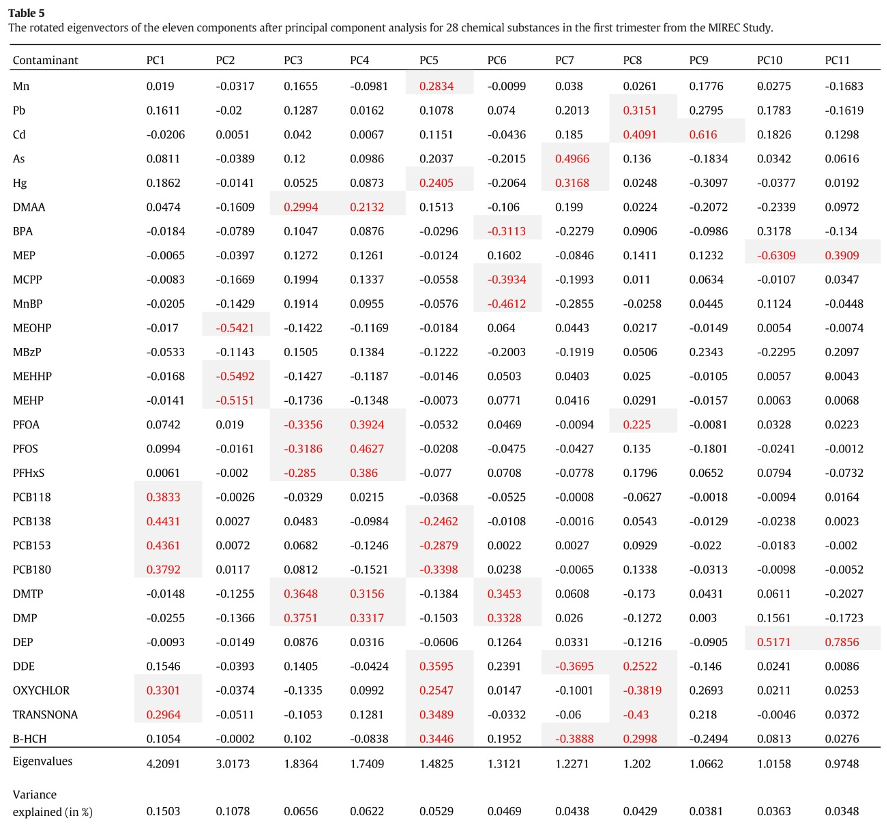
\includegraphics{images/table5.png}
\caption{Loading factors (figure from Lee et al., 2017)}
\end{figure}

The interpretation of such components is not straightforward (the paper does not mention whether a rotation was considered). The first component has higher loadings on PCBs, while the second component has high loadings on DEHP metabolites. All other components have high loadings on specific subsets of exposures, but fail to uniquely identify clusters of exposures within the mixture. For example, to describe exposure to organochlorine pesticides, we find similar loading factors in PC1, PC5, and PC9. Similarly, organophosphate pesticides equivalently load on PC3, PC4, and PC6. As described in the previous paragraphs, this has relevant implications when attempting to evaluate PCA components in a regression model. The following figure presents results from such regression in the paper:

\begin{figure}
\centering
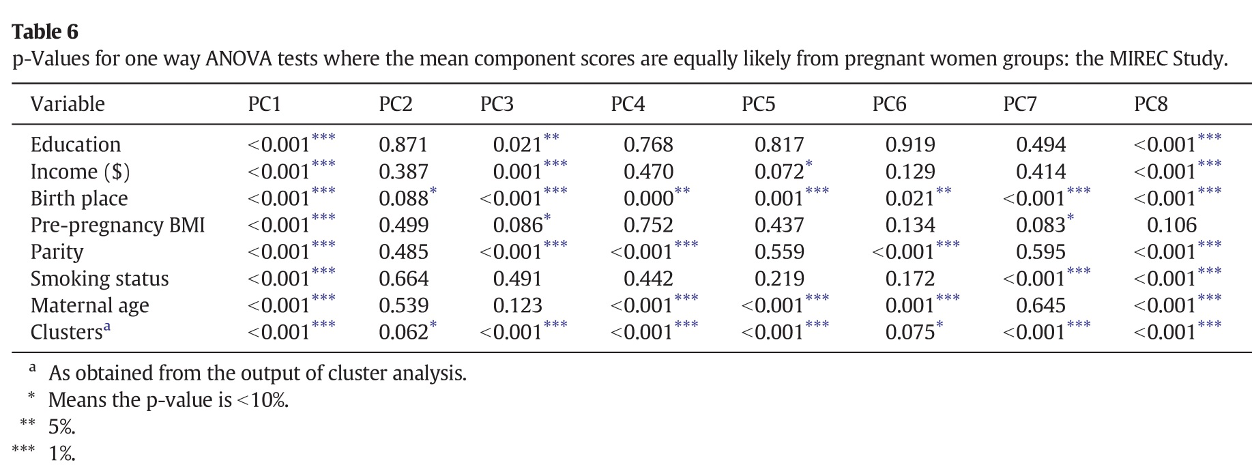
\includegraphics{images/table6.png}
\caption{Regression (figure from Lee et al., 2017)}
\end{figure}

From this table we might be able to conclude that PCBs are associated with the outcome of interest (as they load on PC1), but it is not easy to draw any conclusion about other sets of exposures, whose variability is captured by multiple components. To conclude, the real information that a PCA model is giving us in this example is that the mixture is very complex and we do not observe clearly defined subgroups of exposures based on the correlation structure. In such setting, a PCA analysis might not be the best option to evaluate exposure-outcome associations, and other methods should be considered.

A second interesting example can be found in \citet{sanchez2018urinary}, evaluating metals and socio-demographic characteristics in the HEALS study in Bangladesh. Out of a mixture of 15 metals, a rotated PCA identified 6 principal components explaining 81\% of the total variability. Differently from the previous examples, such components better identify subgroups of exposures (figure).

\begin{figure}
\centering
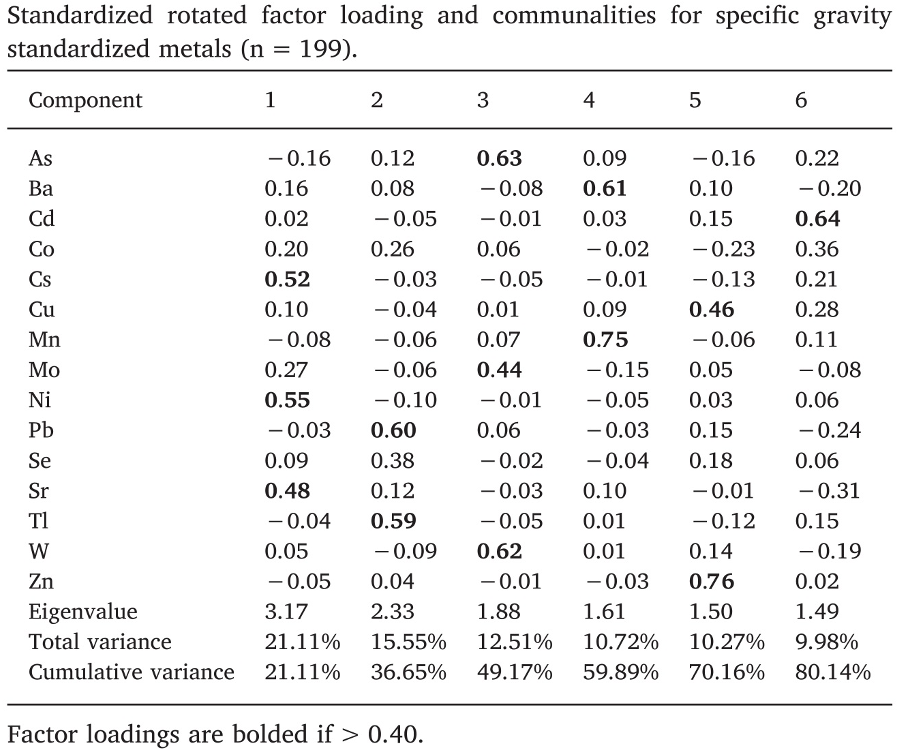
\includegraphics{images/tableaa.png}
\caption{Loading factors (figure from Sanchez et al., 2018)}
\end{figure}

If we look at these loading factors by row, we see that each metal has a high loading factor with one component, and low loadings to all other. For example arsenic (row 1) is described by PC3, cadmium (row 3), by PC6, and so on down to zinc, described by PC5.
In this situation, a regression model with the principal components will have a better interpretation; for example, associations between PC3 and the outcome can be used to retrieve information on the associations between arsenic, molybdenum, and tungsten, on the outcome.

Nevertheless, it is important to note some critical limitations of this approach, that remain valid also when a perfect interpretation can be provided. Let's think of this third principal component that is well describing the variability of arsenic, molybdenum, and tungsten. A regression coefficient linking PC3 with the outcome would only tell us how the subgroup of these 3 exposures is associated with the outcome, but would not inform us on which if the three is driving the association, whether all three exposures have effects in the same direction, nor whether there is any interaction between the three components. Moreover, let's not forget that components are calculated as linear combinations of the exposures and without taking the relationship with the outcome into account.

For these reasons, we can conclude that PCA is very powerful tool to be considered in the preliminary unsupervised assessment of the mixture as it can inform subsequent analyses. On the other hand, using derived components into regression modeling must be done with caution, and is usually outperformed by most supervised approaches that we will describe later.

Finally, it is important to mention that several extensions of the classical PCA have been developed, including a supervised version of the approach. These techniques, however, were developed in other fields and have not gained too much popularity in the context of environmental exposures, where alternative supervised approaches, presented in the following sections, are generally used.

\hypertarget{cluster-analysis}{%
\section{Cluster analysis}\label{cluster-analysis}}

While a principal components analysis can be seen as a way to identify subgroups of exposures (the columns of the mixture matrix) within the mixture based on their correlation structure, another useful exploratory analysis consists in identifying subgroups of individuals (the rows of the data) that share similar exposure profiles. This is commonly done with cluster analysis. Like PCA, cluster analysis requires complete data and standardized variables. To group individuals, a distance measure must be identified, with several options available from standard euclidean distance to distances based on the correlations structure.

\hypertarget{k-means-clustering}{%
\subsection{K-means clustering}\label{k-means-clustering}}

The most common approach to partition the data into clusters, is an unsupervised approach called k-means clustering. This method classifies objects in \(k\) groups (i.e., clusters), so that individuals within the same cluster are as similar as possible, while individuals from different clusters are as dissimilar as possible. To achieve that, clusters are defined in a way that minimizes within-cluster variation. A simple algorithm for k-clustering proceeds as follow

\begin{enumerate}
\def\labelenumi{\arabic{enumi}.}
\tightlist
\item
  Pre-specify \(k\), the number of clusters
\item
  Select \(k\) random individuals as center for each cluster and define the centroids, vectors of length \(p\) that contain the means of all variables for the observation in the cluster. In our context, the \(p\) variables are the components of our mixture of interest
\item
  Define a distance measure. The standard choice is the euclidean distance defined as \((x_i-\mu_k)\) i, for each individual in the study (\(x_i\)) and each cluster center (\(\mu_k\)).
\item
  Assign each individual to the closest centroid
\item
  For each of the \(k\) clusters update the cluster centroid by calculating the new mean values of all the data points in the cluster
\item
  Iteratively update the previous 2 steps until the the cluster assignments stop changing or the maximum number of iterations is reached. By default, the R software uses 10 as the default value for the maximum number of iterations.
\end{enumerate}

This simple algorithm minimizes the total within-cluster variation, defined for each cluster \(C_k\) as the sum of squared euclidean distances within that cluster \(W(C_k)=\sum_{x_i\in C_k}(x_i-\mu_k)^2\)

Since k-mean clustering requires the user to specify the number of groups, it is important to assess the optimal number of groups. A simple technique is to use the elbow method, similar to the one presented for PCA, which consists in plotting the within-cluster sum of squares versus the number of clusters, and locating the bend in the plot.

\hypertarget{k-means-in-r}{%
\subsection{K-means in R}\label{k-means-in-r}}

We can compute k-means in R with the \texttt{kmeans} function within the \texttt{cluster} package. Here we are selecting 3 groups, also using the \texttt{nstart} option that will attempts multiple initial configurations (here 20) and report the best one.

\begin{Shaded}
\begin{Highlighting}[]
\NormalTok{k3 }\OtherTok{\textless{}{-}} \FunctionTok{kmeans}\NormalTok{(X, }\AttributeTok{centers =} \DecValTok{3}\NormalTok{, }\AttributeTok{nstart =} \DecValTok{20}\NormalTok{)}
\NormalTok{k3}
\end{Highlighting}
\end{Shaded}

The option \texttt{fviz\_cluster} provides a nice graphical representation of the groupings. If there are more than two variables \texttt{fviz\_cluster} will perform principal component analysis (PCA) and plot the data points according to the first two principal components that explain the majority of the variance.

\begin{Shaded}
\begin{Highlighting}[]
\FunctionTok{fviz\_cluster}\NormalTok{(k3, }\AttributeTok{data =}\NormalTok{ X)}
\end{Highlighting}
\end{Shaded}

\begin{figure}[H]

{\centering 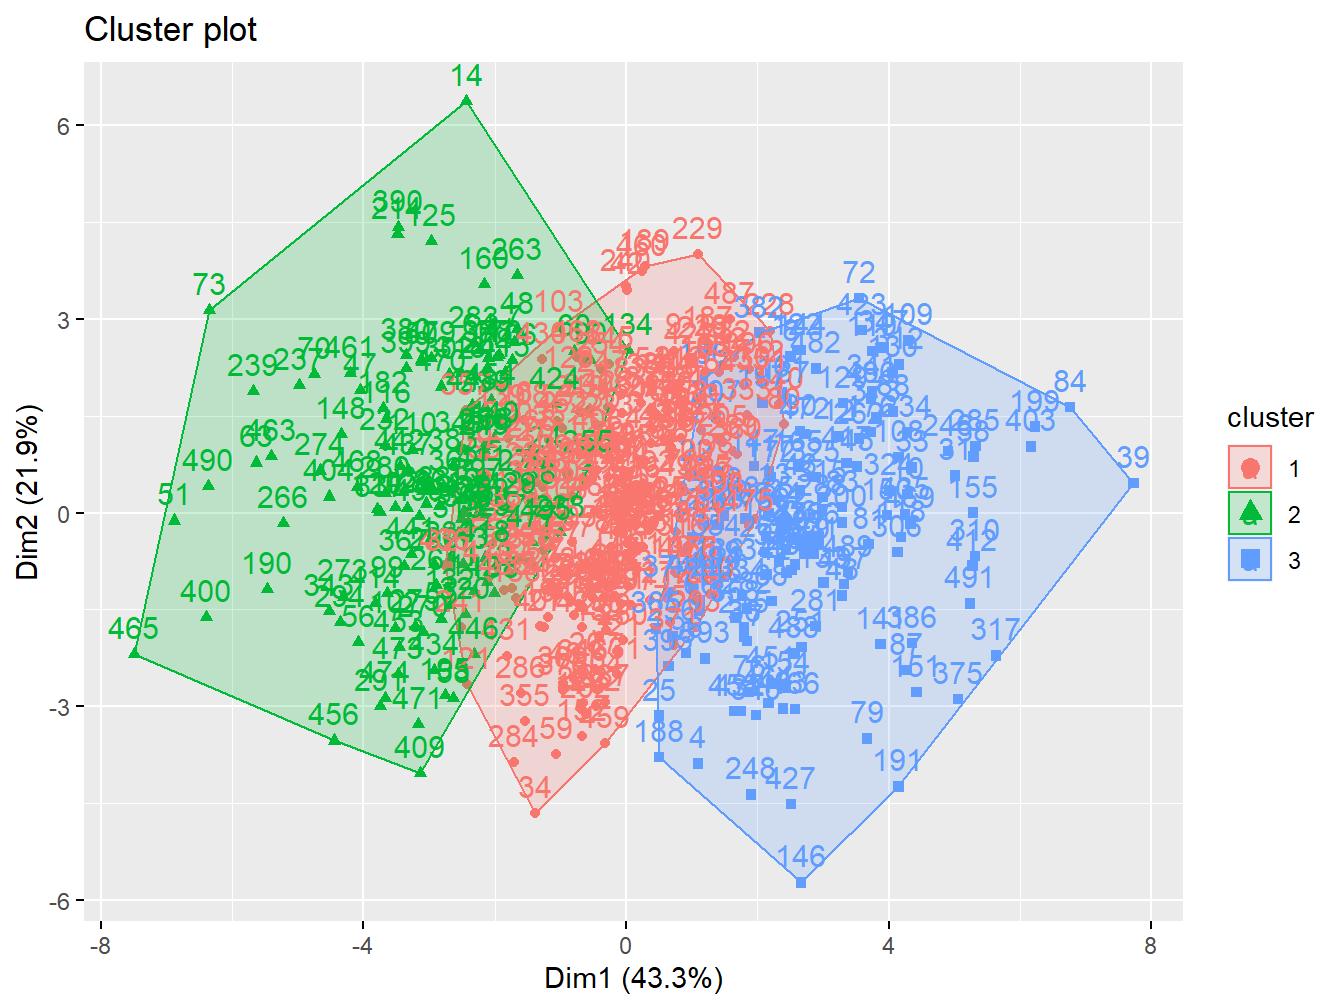
\includegraphics[width=0.8\linewidth]{bookdown-demo_files/figure-latex/figurecl-1} 

}

\caption{Cluster analysis with 3 groups}\label{fig:figurecl}
\end{figure}

Here we can test more

\begin{Shaded}
\begin{Highlighting}[]
\NormalTok{k2 }\OtherTok{\textless{}{-}} \FunctionTok{kmeans}\NormalTok{(X, }\AttributeTok{centers =} \DecValTok{2}\NormalTok{, }\AttributeTok{nstart =} \DecValTok{20}\NormalTok{)}
\NormalTok{k4 }\OtherTok{\textless{}{-}} \FunctionTok{kmeans}\NormalTok{(X, }\AttributeTok{centers =} \DecValTok{4}\NormalTok{, }\AttributeTok{nstart =} \DecValTok{20}\NormalTok{)}
\NormalTok{k5 }\OtherTok{\textless{}{-}} \FunctionTok{kmeans}\NormalTok{(X, }\AttributeTok{centers =} \DecValTok{5}\NormalTok{, }\AttributeTok{nstart =} \DecValTok{20}\NormalTok{)}
\end{Highlighting}
\end{Shaded}

\begin{Shaded}
\begin{Highlighting}[]
\NormalTok{p1 }\OtherTok{\textless{}{-}} \FunctionTok{fviz\_cluster}\NormalTok{(k2, }\AttributeTok{geom =} \StringTok{"point"}\NormalTok{, }\AttributeTok{data =}\NormalTok{ X) }\SpecialCharTok{+} \FunctionTok{ggtitle}\NormalTok{(}\StringTok{"k = 2"}\NormalTok{)}
\NormalTok{p2 }\OtherTok{\textless{}{-}} \FunctionTok{fviz\_cluster}\NormalTok{(k3, }\AttributeTok{geom =} \StringTok{"point"}\NormalTok{,  }\AttributeTok{data =}\NormalTok{ X) }\SpecialCharTok{+} \FunctionTok{ggtitle}\NormalTok{(}\StringTok{"k = 3"}\NormalTok{)}
\NormalTok{p3 }\OtherTok{\textless{}{-}} \FunctionTok{fviz\_cluster}\NormalTok{(k4, }\AttributeTok{geom =} \StringTok{"point"}\NormalTok{,  }\AttributeTok{data =}\NormalTok{ X) }\SpecialCharTok{+} \FunctionTok{ggtitle}\NormalTok{(}\StringTok{"k = 4"}\NormalTok{)}
\NormalTok{p4 }\OtherTok{\textless{}{-}} \FunctionTok{fviz\_cluster}\NormalTok{(k5, }\AttributeTok{geom =} \StringTok{"point"}\NormalTok{,  }\AttributeTok{data =}\NormalTok{ X) }\SpecialCharTok{+} \FunctionTok{ggtitle}\NormalTok{(}\StringTok{"k = 5"}\NormalTok{)}

\FunctionTok{grid.arrange}\NormalTok{(p1, p2, p3, p4, }\AttributeTok{nrow =} \DecValTok{2}\NormalTok{)}
\end{Highlighting}
\end{Shaded}

\begin{figure}[H]

{\centering 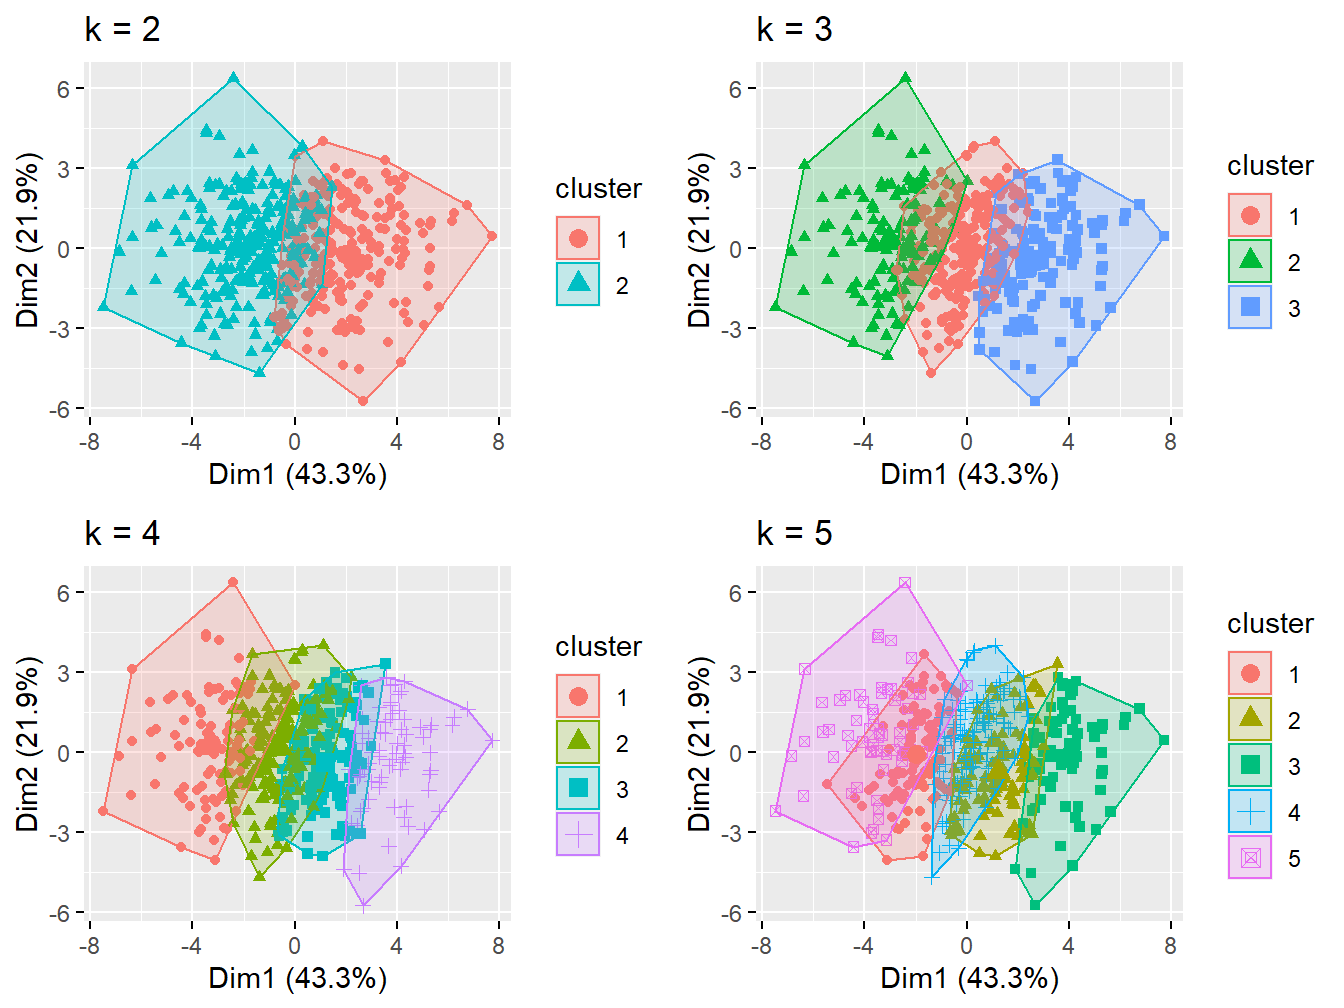
\includegraphics[width=0.8\linewidth]{bookdown-demo_files/figure-latex/figurecl2-1} 

}

\caption{Cluster analysis with 2-5 groups}\label{fig:figurecl2}
\end{figure}

The elbow plot can tell us how many groups optimally classify individuals. This figure shows that 2 might be enough.

\begin{Shaded}
\begin{Highlighting}[]
\FunctionTok{set.seed}\NormalTok{(}\DecValTok{123}\NormalTok{)}
\FunctionTok{fviz\_nbclust}\NormalTok{(X, kmeans, }\AttributeTok{method =} \StringTok{"wss"}\NormalTok{)}
\end{Highlighting}
\end{Shaded}

\begin{figure}[H]

{\centering 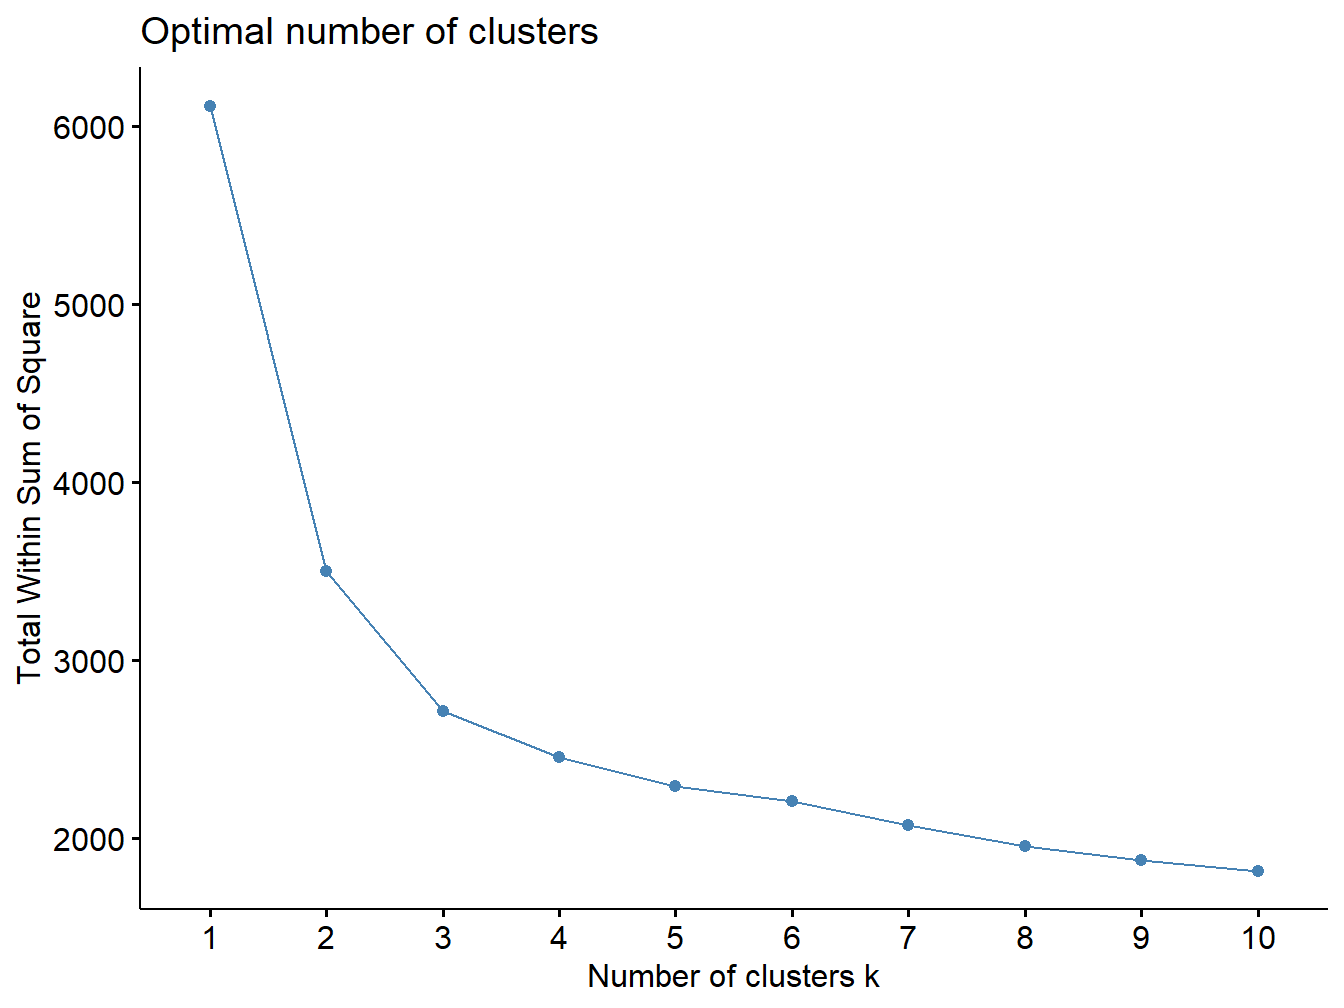
\includegraphics[width=0.8\linewidth]{bookdown-demo_files/figure-latex/figurecl3-1} 

}

\caption{Elbow plot}\label{fig:figurecl3}
\end{figure}

\hypertarget{cluster-analysis-to-simplify-descriptive-statistics-presentation}{%
\subsection{Cluster analysis to simplify descriptive statistics presentation}\label{cluster-analysis-to-simplify-descriptive-statistics-presentation}}

One of the advantages of clustering individuals is to provide a better presentation of descriptive statistics and univariate associations with other covariates in the dataset prior to formal analysis (what is commonly done in table 1 of a scientific manuscript). First, let's define the exposure profiles by evaluating the distribution of original exposures in the clusters:

\begin{tabular}[t]{llll}
\toprule
  & 1 & 2 & Overall\\
\midrule
 & (N=236) & (N=264) & (N=500)\\
\addlinespace[0.3em]
\multicolumn{4}{l}{\textbf{x1}}\\
\hspace{1em}Mean (SD) & 1.04 (0.718) & 1.01 (0.684) & 1.02 (0.699)\\
\hspace{1em}Median [Min, Max] & 1.04 [-1.18, 2.49] & 1.02 [-0.936, 2.89] & 1.03 [-1.18, 2.89]\\
\addlinespace[0.3em]
\multicolumn{4}{l}{\textbf{x2}}\\
\hspace{1em}Mean (SD) & -2.05 (0.765) & -2.18 (0.759) & -2.12 (0.764)\\
\hspace{1em}Median [Min, Max] & -2.10 [-4.32, 0.193] & -2.23 [-4.01, -0.291] & -2.14 [-4.32, 0.193]\\
\addlinespace[0.3em]
\multicolumn{4}{l}{\textbf{x3}}\\
\hspace{1em}Mean (SD) & 2.48 (0.885) & 0.291 (0.907) & 1.32 (1.41)\\
\hspace{1em}Median [Min, Max] & 2.36 [0.993, 5.43] & 0.511 [-2.33, 1.83] & 1.33 [-2.33, 5.43]\\
\addlinespace[0.3em]
\multicolumn{4}{l}{\textbf{x4}}\\
\hspace{1em}Mean (SD) & 3.49 (0.867) & 1.33 (0.889) & 2.35 (1.39)\\
\hspace{1em}Median [Min, Max] & 3.39 [1.93, 6.36] & 1.51 [-1.36, 2.92] & 2.32 [-1.36, 6.36]\\
\addlinespace[0.3em]
\multicolumn{4}{l}{\textbf{x5}}\\
\hspace{1em}Mean (SD) & 1.86 (1.03) & -0.645 (1.04) & 0.537 (1.62)\\
\hspace{1em}Median [Min, Max] & 1.81 [-0.311, 4.85] & -0.459 [-4.22, 1.42] & 0.504 [-4.22, 4.85]\\
\addlinespace[0.3em]
\multicolumn{4}{l}{\textbf{x6}}\\
\hspace{1em}Mean (SD) & 1.52 (0.892) & 0.326 (0.815) & 0.891 (1.04)\\
\hspace{1em}Median [Min, Max] & 1.50 [-0.564, 3.76] & 0.356 [-2.12, 2.25] & 0.833 [-2.12, 3.76]\\
\addlinespace[0.3em]
\multicolumn{4}{l}{\textbf{x7}}\\
\hspace{1em}Mean (SD) & 1.51 (0.556) & 1.15 (0.490) & 1.32 (0.552)\\
\hspace{1em}Median [Min, Max] & 1.51 [0.216, 2.94] & 1.18 [-0.356, 2.50] & 1.33 [-0.356, 2.94]\\
\addlinespace[0.3em]
\multicolumn{4}{l}{\textbf{x8}}\\
\hspace{1em}Mean (SD) & 3.39 (0.737) & 2.08 (0.767) & 2.70 (0.999)\\
\hspace{1em}Median [Min, Max] & 3.31 [1.65, 5.92] & 2.10 [-0.268, 4.84] & 2.69 [-0.268, 5.92]\\
\addlinespace[0.3em]
\multicolumn{4}{l}{\textbf{x9}}\\
\hspace{1em}Mean (SD) & 1.45 (0.529) & 1.21 (0.571) & 1.32 (0.564)\\
\hspace{1em}Median [Min, Max] & 1.43 [0.0496, 2.70] & 1.25 [-0.328, 2.98] & 1.34 [-0.328, 2.98]\\
\addlinespace[0.3em]
\multicolumn{4}{l}{\textbf{x10}}\\
\hspace{1em}Mean (SD) & 3.46 (0.690) & 2.86 (0.683) & 3.14 (0.748)\\
\hspace{1em}Median [Min, Max] & 3.42 [1.69, 5.26] & 2.81 [1.07, 4.66] & 3.13 [1.07, 5.26]\\
\addlinespace[0.3em]
\multicolumn{4}{l}{\textbf{x11}}\\
\hspace{1em}Mean (SD) & 5.61 (0.638) & 4.81 (0.674) & 5.19 (0.769)\\
\hspace{1em}Median [Min, Max] & 5.53 [3.98, 7.80] & 4.80 [2.62, 6.71] & 5.21 [2.62, 7.80]\\
\addlinespace[0.3em]
\multicolumn{4}{l}{\textbf{x12}}\\
\hspace{1em}Mean (SD) & 0.466 (0.337) & 0.493 (0.347) & 0.481 (0.342)\\
\hspace{1em}Median [Min, Max] & 0.443 [-0.429, 1.15] & 0.507 [-0.481, 1.49] & 0.483 [-0.481, 1.49]\\
\addlinespace[0.3em]
\multicolumn{4}{l}{\textbf{x13}}\\
\hspace{1em}Mean (SD) & 0.530 (0.348) & 0.578 (0.348) & 0.555 (0.349)\\
\hspace{1em}Median [Min, Max] & 0.514 [-0.371, 1.42] & 0.570 [-0.355, 1.65] & 0.552 [-0.371, 1.65]\\
\addlinespace[0.3em]
\multicolumn{4}{l}{\textbf{x14}}\\
\hspace{1em}Mean (SD) & 1.79 (0.549) & 0.881 (0.562) & 1.31 (0.719)\\
\hspace{1em}Median [Min, Max] & 1.79 [0.373, 3.55] & 0.879 [-1.29, 2.64] & 1.31 [-1.29, 3.55]\\
\bottomrule
\end{tabular}

We see that individuals in the first cluster have higher exposure levels to most of the included contaminants, so we could define cluster 1 as ``high'' and cluster 2 as ``low'' exposure. Next, we can see the distribution of outcome and covariates by clustering.

\begin{tabular}[t]{llll}
\toprule
  & 1 & 2 & Overall\\
\midrule
 & (N=236) & (N=264) & (N=500)\\
\addlinespace[0.3em]
\multicolumn{4}{l}{\textbf{Outcome}}\\
\hspace{1em}Mean (SD) & 4.19 (0.619) & 3.64 (0.569) & 3.90 (0.653)\\
\hspace{1em}Median [Min, Max] & 4.17 [2.66, 6.00] & 3.62 [2.25, 5.22] & 3.87 [2.25, 6.00]\\
\addlinespace[0.3em]
\multicolumn{4}{l}{\textbf{Poverty index}}\\
\hspace{1em}Mean (SD) & 2.26 (1.59) & 1.90 (1.63) & 2.07 (1.62)\\
\hspace{1em}Median [Min, Max] & 2.18 [-1.87, 7.62] & 1.87 [-2.47, 5.95] & 2.08 [-2.47, 7.62]\\
\addlinespace[0.3em]
\multicolumn{4}{l}{\textbf{Age}}\\
\hspace{1em}Mean (SD) & 46.4 (18.8) & 14.4 (17.9) & 29.5 (24.3)\\
\hspace{1em}Median [Min, Max] & 45.2 [1.01, 102] & 15.1 [-38.3, 54.3] & 28.6 [-38.3, 102]\\
\bottomrule
\end{tabular}

We see that both z1, z2, z3, as well as the outcome are higher among individuals in cluster 1, who are characterized by the exposure profile presented in the previous table.

\hypertarget{regression-based-approaches}{%
\chapter{Regression-based approaches}\label{regression-based-approaches}}

The previous section described a set of unsupervised techniques for the analysis of environmental mixtures, used to process the complex data before further analyses and to address well defined research questions related to the identification of common patterns of exposures or clustering of individuals based on exposure profiles. In the context of environmental health studies, however, this only represents the first (yet critical) step of analysis. The ultimate goal of most research in the field is in fact to investigate whether exposure to mixtures of environmental factors are associated with a given health outcome, and possibly whether these associations represent causal effects. Epidemiologists are usually trained to address these questions using regression-based techniques such as generalized linear models, for binary and continuous outcomes, or parametric and semi-parametric regression techniques for survival data, with time-to-event outcomes. Nevertheless, environmental exposures often present complex settings that require handling regression with care. The goal of this section is to present the use of classical regression techniques (i.e.~ordinary least squares (OLS)) in mixtures modeling, its limitations, and introduce some important extensions of OLS that allow overcoming these shortcomings.

\hypertarget{ols-regression}{%
\section{OLS regression}\label{ols-regression}}

\hypertarget{single-regression-ewas}{%
\subsection{Single regression (EWAS)}\label{single-regression-ewas}}

A simple way to assess the association between a set of \(p\) environmental exposures (\(X_1 - X_p\)) and a given outcome \(Y\) is to build \(p\) different regression models, one for each exposure (the approach that we previously described as ``one-at-the-time''). Each model can be further adjusted for potential confounders of each exposure-outcome association. For example, is \(Y\) was a continuous exposure, we could fit a set of linear regression models such as: \(E[Y|X_1,C]=\beta_0+\beta_1 \cdot X_1 + \beta\cdot C\). The implicit assumption of this modeling procedure is that, for each element of the mixture, the other components do not act as confounders of the exposure-outcome association, as depicted in this DAG:
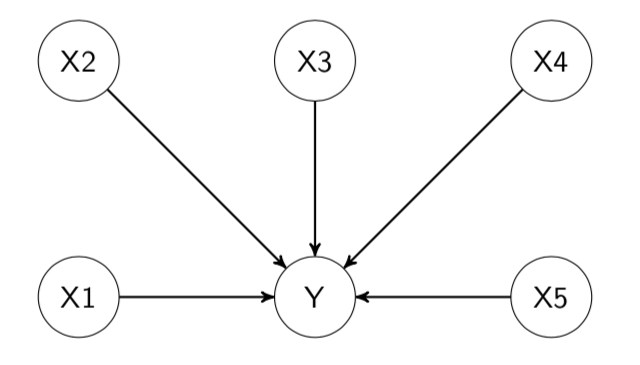
\includegraphics{images/dag1.png}

When evaluating a set of environmental exposures, this procedure of fitting a set of independent regression models is usually referred to as environment-wide association study (EWAS, Patel et al.~2010). This approach usually requires correcting for multiple comparisons using wither the Bonferroni approach or the false discovery rate (FDR).

The following table reports results from fitting independent linear regression models (here without any adjustment for multiple comparisons) in our illustrative example with 14 exposures:

Dependent variable:

y

(1)

(2)

x12

0.294*** (0.169, 0.420)

x13

0.238*** (0.112, 0.364)

z1

-0.010 (-0.036, 0.016)

-0.010 (-0.037, 0.016)

z2

0.013*** (0.011, 0.015)

0.013*** (0.011, 0.015)

z3

-0.610*** (-0.694, -0.525)

-0.612*** (-0.698, -0.527)

Constant

3.712*** (3.592, 3.833)

3.725*** (3.596, 3.854)

Observations

500

500

Note:

\emph{p\textless0.1; \textbf{p\textless0.05; }}p\textless0.01

These results seem to indicate that all exposures are independently associated with the outcome (many coefficients fail to reach the conventional threshold of statistical significance, but we will stick on the magnitude and direction of the associations for this illustrative example).

\hypertarget{multiple-regression}{%
\subsection{Multiple regression}\label{multiple-regression}}

Results from independent linear regression are hampered by the strong assumption that mixture components do not act as confounders of the association between each other component and the outcome of interest. This assumption, however, is very seldom met in practice. A common situation, for example, is that two or more constituents of the mixture share one or more source, which usually results in moderate to high levels of correlation between exposures. Using DAGs, we can depict this situation with the following:

\begin{figure}
\centering
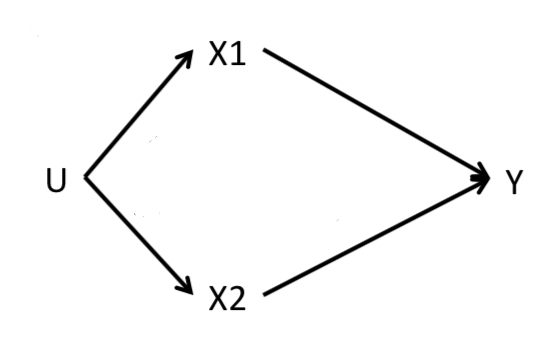
\includegraphics{images/dag2.png}
\caption{DAG for 2 exposures}
\end{figure}

In this situation, a statistical model evaluating the association between \(X_1\) and \(Y\) will need to adjust for \(X_2\) to reduce the impact of bias due to residual confounding. In general, when any level of correlation exists between two mixture components, we do expect them to act as confounders of the association between the other exposure and the outcome. This implies that results from independent linear regressions are likely biased due to uncontrolled confounding. In our illustrative example, for instance, we know that \(X_{12}\) and \(X_{13}\) are highly correlated; results from independent linear regressions indicated that both exposures are positively associated with the outcome, but we now know that these coefficients are probably biased. Mutually adjusting for the two exposures in the same statistical model is therefore required to account for such confounding and possibly identify whether both exposures are really associated with the outcome, or if the real driver of the association is just one of the two. Note that both situations are realistic: we might have settings where a specific exposure is biologically harmful (say \(X_{12}\)), and the association between the correlated one (\(X_{13}\)) and the outcome was a spurious result due to this high correlation, as well as settings where both exposures are really associated with the outcome (maybe because it is the source of exposure to have a direct effect). We need statistical methodologies to be able to detect and distinguish these possible scenarios.

The most intuitive way to account for co-confounding between mixture components is to mutually adjust for all exposures in the same regression model:

\[E[Y|X,C]=\beta_0+\sum_{i=1}^p\beta_i \cdot X_i + \beta \cdot C\]

The following table presents results from a multiple regression that includes the 14 exposures in our example, as well as results from the independent models for \(X_{12}\) and \(X_{13}\) for comparison

We can compare results from different models using the stargazer package. Let's use it to compare results from the full model, and the models for \(X_{12}\) and \(X_{13}\) alone:

Dependent variable:

y

(1)

(2)

(3)

x1

0.058* (-0.007, 0.123)

x2

0.018 (-0.043, 0.080)

x3

-0.030 (-0.232, 0.173)

x4

0.053 (-0.170, 0.275)

x5

0.004 (-0.080, 0.088)

x6

0.060** (0.001, 0.119)

x7

-0.031 (-0.153, 0.091)

x8

0.017 (-0.063, 0.097)

x9

0.025 (-0.090, 0.140)

x10

0.052 (-0.039, 0.144)

x11

0.049 (-0.052, 0.151)

x12

0.222 (-0.071, 0.515)

0.294*** (0.169, 0.420)

x13

-0.083 (-0.382, 0.216)

0.238*** (0.112, 0.364)

x14

0.054 (-0.047, 0.154)

z1

0.006 (-0.021, 0.032)

-0.010 (-0.036, 0.016)

-0.010 (-0.037, 0.016)

z2

0.006*** (0.003, 0.010)

0.013*** (0.011, 0.015)

0.013*** (0.011, 0.015)

z3

-0.609*** (-0.696, -0.522)

-0.610*** (-0.694, -0.525)

-0.612*** (-0.698, -0.527)

Constant

3.265*** (2.800, 3.730)

3.712*** (3.592, 3.833)

3.725*** (3.596, 3.854)

Observations

500

500

500

Note:

\emph{p\textless0.1; \textbf{p\textless0.05; }}p\textless0.01

\hypertarget{the-problem-of-multicollinearity}{%
\subsection{The problem of Multicollinearity}\label{the-problem-of-multicollinearity}}

Results from the multiple regression are not consistent with those obtained from independent regression models, especially (and unsurprisingly) for those exposures that showed high levels of correlations. For example, within the exposure cluster \(X_{12}-X_{13}\), the multiple regression model suggests that only \(X_{12}\) is associated with the outcome, while the coefficient of \(X_{13}\) is strongly reduced. Something similar happens for the \(X_3-X_4-X_5\) cluster, where only \(X_4\) remains associated with \(Y\). Can we safely conclude that \(X_{12}\) and \(X_4\) are associated with \(Y\) and that the other results were biased due to uncontrolled confounders? Before addressing this question, let's take a look at this published paper where we evaluated the performance of several statistical models to evaluate the association between a mixture of 8 phthalate metabolites and birth weight in a pregnancy cohort (\citet{chiu2018evaluating}). The following table presents results from 8 independent regressions and a multiple regression model. The next figure presents instead the correlation plot of the 8 metabolites.

\begin{longtable}[]{@{}lcrrr@{}}
\toprule
Metabolite & \(\beta\) (one at the time) & p-value & \(\beta\) (mutually adjusted) & p-value \\
\midrule
\endhead
MiBP & -20.0 & 0.51 & -6.8 & 0.84 \\
MBzP & -24.7 & 0.34 & -18.7 & 0.53 \\
MEOHP & -23.7 & 0.33 & 247.1 & 0.11 \\
MnBP & -28.5 & 0.31 & -6.5 & 0.86 \\
MEHHP & -28.2 & 0.24 & -127.4 & 0.36 \\
MECPP & -32.6 & 0.20 & -82.8 & 0.32 \\
MEP & -27.1 & 0.18 & 25.0 & 0.24 \\
MEHP & -36.8 & 0.10 & -59.0 & 0.18 \\
\bottomrule
\end{longtable}

\begin{figure}
\centering
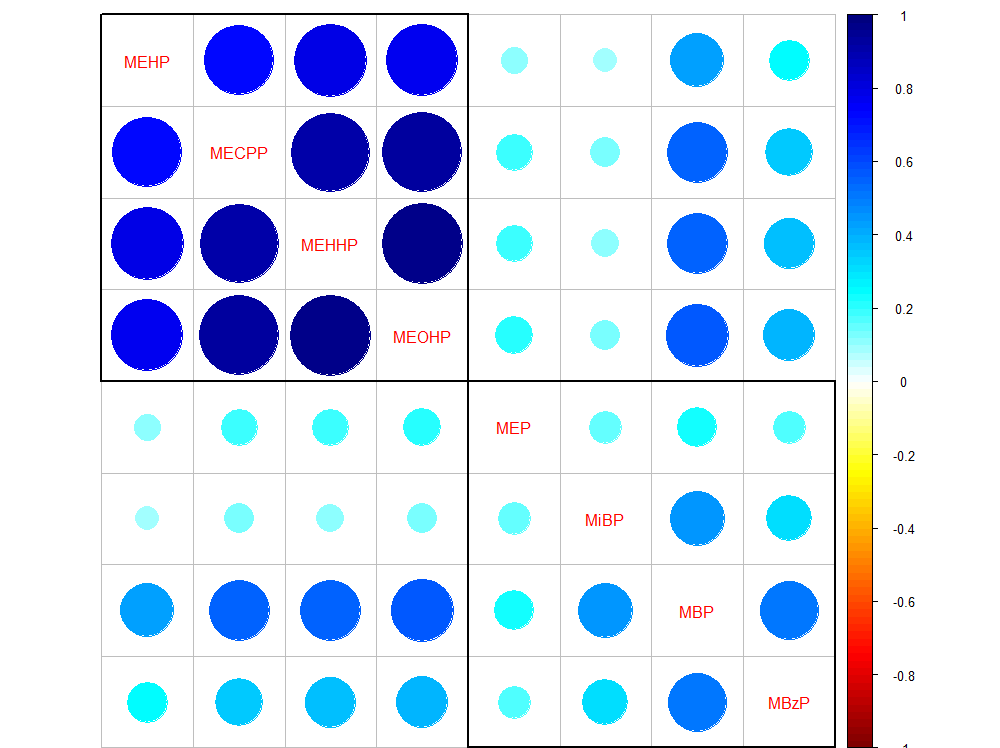
\includegraphics{images/Rplot02.png}
\caption{Correlation plot from Chiu et al.}
\end{figure}

While we were expecting results from the two approaches to be different in the presence of high correlations, the coefficients obtained from the multiple regression leave room to a lot of skepticism. For example, the coefficients for MEOHP and MEHHP, when evaluated together, change respectively from -24 to 247, and from -28 to -127. Are these results reliable? Are we getting any improvement from to the biased results that we obtained from independent linear regressions?

The most common problem that arises when using multiple regression to investigate mixture-outcome association is multicollinearity (or simply collinearity). This occurs when independent variables in a regression model are correlated, with stronger consequences the higher the correlation. More specifically, a high correlation between two predictors simultaneously included in a regression model will decrease the precision of their estimates and increase their standard errors. If the correlation between two covariates (say \(X_1\) and \(X_2\)) is very high, then one is a pretty accurate linear predictor of the other. Collinearity does not influence the overall performance of the model, but has an important impact on individual predictors. In general (as a rule of thumb), given two predictors \(X_1\) and \(X_2\) that are associated with the outcome (\(\beta=0.2\) for both) when their correlation is equal to 0, the estimates in a linear model will be impacted by \(\rho(X_1, X_2)\) as in this figure:
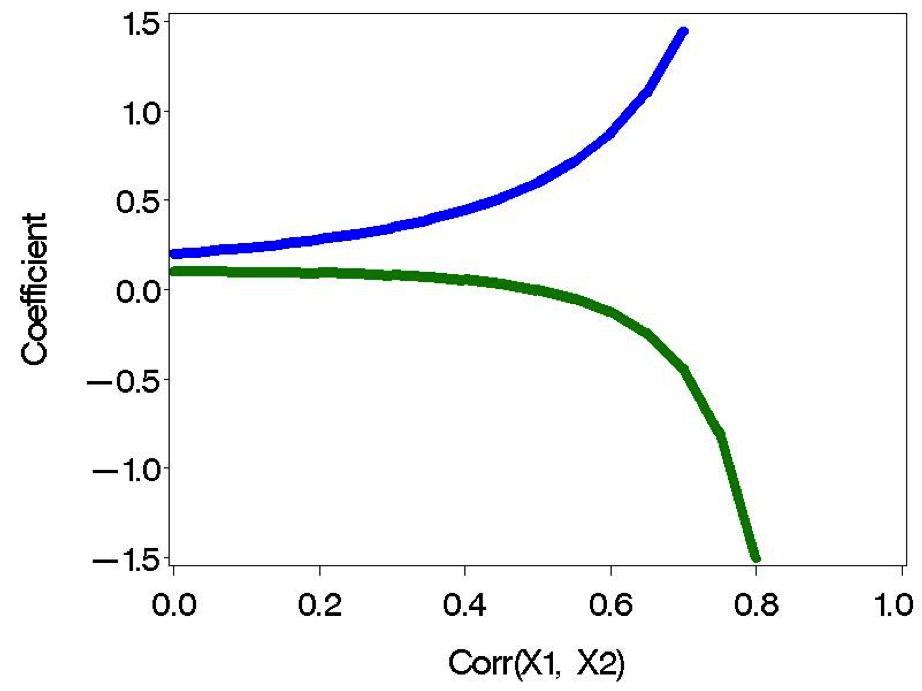
\includegraphics{images/revparadox.png}

This issue, usually referred to as reverse paradox (the coefficients of 2 correlated covariates will inflate in opposite directions), is clearly affecting results from the paper presented above (the coefficients of highly correlated phthalate metabolites are either extremely large or extremely small), and possibly also results from the illustrative example (coefficients from correlated variables have opposite signs). Nevertheless, it should be noted that high correlation does not automatically imply that coefficients will be inflated. In another example (\citet{bellavia2019urinary}), for instance, we evaluated a mixture of three highly correlated parabens compounds, yet results from multiple regression were in line to those obtained from other mixture modeling techniques.

To quantify the severity of multicollinearity in a regression analysis one should calculate the Variance Inflation Factor (VIF). The VIF provides a measure of how much the variance of an estimated regression coefficient is increased because of collinearity. For example, if the VIF for a given predictors were 4, than the standard error of that predictors is 2 times larger than if that predictor had 0 correlation with other variables. As a rule of thumb, VIFs above 4 should set the alarm off, as they indicate that those coefficients are likely affected by the high correlations between them and other covariates in the model. The following table shows VIFs in our illustrative example, indicating that our results are deeply affected by multicollinearity. In this situation, alternative modeling options should be pursued.

\begin{table}

\caption{\label{tab:unnamed-chunk-15}VIFs}
\centering
\begin{tabular}[t]{l|r}
\hline
  & x\\
\hline
x1 & 1.235658\\
\hline
x2 & 1.317951\\
\hline
x3 & 49.479946\\
\hline
x4 & 58.241935\\
\hline
x5 & 11.256382\\
\hline
x6 & 2.271043\\
\hline
x7 & 2.722583\\
\hline
x8 & 3.892965\\
\hline
x9 & 2.553431\\
\hline
x10 & 2.810535\\
\hline
x11 & 3.694404\\
\hline
x12 & 6.085748\\
\hline
x13 & 6.557098\\
\hline
x14 & 3.152092\\
\hline
z1 & 1.139690\\
\hline
z2 & 4.784064\\
\hline
z3 & 1.135437\\
\hline
\end{tabular}
\end{table}

\hypertarget{penalized-regression-approaches}{%
\section{Penalized regression approaches}\label{penalized-regression-approaches}}

An important set of models that can be very useful in the context of environmental mixtures are penalized regression approaches. These methods are directly built as extensions of standard OLS by incorporating a penalty in the loss function (hence the name). Their popularity in environmental epidemiology is due to the fact that this penalization procedure tends to decrease the influence of collinearity by targeting the overall variability of the model, thus improving the performance of the regression in the presence of high levels of correlations between included covariates. As always, however, everything comes for a price, and the improvement in the variance is achieved by introducing some bias (specifically, coefficients will be shrinked towards zero, reason why these approaches are also referred to as shrinkage procedures).

\hypertarget{bias-variance-tradeoff}{%
\subsection{Bias-variance tradeoff}\label{bias-variance-tradeoff}}

The word bias usually triggers epidemiologists' ears, so it is important to understand what we mean by ``introducing some bias'' and how this can be beneficial in our context. To do so, let's begin by refreshing the basic math behind the estimation of a classical multiple regression. In linear regression modeling, we aim at predicting \(n\) observations of the response variable, \(Y\), with a linear combination of \(m\) predictor variables, \(X\), and a normally distributed error term with variance \(\sigma^2\):
\[Y=X\beta+\epsilon\]
\[\epsilon\sim N(0, \sigma^2)\]

We need a rule to estimate the parameters, \(\beta\), from the sample, and a standard choice to do so is by using ordinary least square (OLS), which produce estimates \(\hat{\beta}\) by minimizing the sum of squares of residuals is as small as possible. In other words, we minimize the following loss function:

\[L_{OLS}(\hat{\beta})=\sum_{i=1}^n(y_i-x_i'\hat{\beta})^2=\|y-X\hat{\beta}\|^2\]

Using matrix notation, the estimate turns out to be :

\[\hat{\beta}_{OLS}=(X'X)^{-1}(X'Y)\]

To evaluate the performance of an estimator, there are two critical characteristics to be considered: its bias and its variance. The bias of an estimator measures the accuracy of the estimates:

\[Bias(\hat{\beta}_{OLS})=E(\hat{\beta}_{OLS})-\beta\]

The variance, on the other hand, measures the uncertainty of the estimates:

\[Var(\hat{\beta}_{OLS})=\sigma^2(X'X)^{-1}\]

Think of the estimator as an olympic archer:
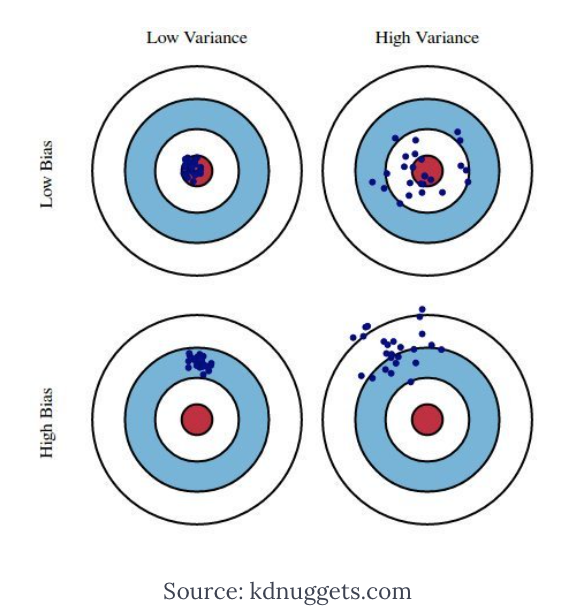
\includegraphics{images/archery.png}

The best performer will be an archer with low bias and low variance (top-left), who consistently aims the target for every estimate. An archer with low bias but high variance will be the one who will shoot inconsistently around the center (top-right), but we may also have an archer with high bias and low variance, who is extremely precise in consistently shooting at the wrong target (bottom-left). Now, the OLS estimator is an archer who is designed to be unbiased, but in certain situations might have a very high variance, situation that commonly happens when collinearity is a threat, as documented by the inflation in the variance calculated by the VIF.

To assess the overall performance an estimator by taking into account both bias and variance, one can look at the Mean Squared Error (MSE), defined as the sum of Variance and squared Bias.

\[MSE=\frac{1}{n}\sum_{i=1}^n(Y_i-\hat{Y_i})^2=Var(\hat{\beta})+Bias^2(\hat{\beta})\]

The basic idea of bias-variance tradeoff is to introduce some bias in order to minimize the mean squared error in those situation where the performances of OLS are affected by high variance. This is achieved by augmenting the loss function by introducing a penalty. While there are several ways of achieving this, we will here focus on 3 common penalty functions that originate Ridge, LASSO, and Elastic-Net regression, with the latter being a generalized version of the previous 2.

\hypertarget{ridge-regression}{%
\subsection{Ridge regression}\label{ridge-regression}}

Ridge regression augments the OLS loss function as to not only minimize the sum of squared residuals, but also penalize the size of the parameter estimates, shrinking them towards zero

\[L_{ridge}(\hat{\beta})=\sum_{i=1}^n(y_i-x_i'\hat{\beta})^2+\lambda\sum_{j=1}^m\hat{\beta}_j^2=\|y-X\hat{\beta}\|^2+\lambda\|\hat{\beta}\|^2\]

Minimizing this equation provides this solution for the parameters estimation:
\[\hat{\beta}_{ridge}=(X'X+\lambda I)^{-1}(X'Y)\]
where \(\lambda\) is the penalty and \(I\) an identity matrix

We can notice that: As \(\lambda\rightarrow 0\), \(\hat{\beta}_{ridge}\rightarrow\hat{\beta}_{OLS}\), while as \(\lambda\rightarrow \infty\), \(\hat{\beta}_{ridge}\rightarrow 0\). In words, setting \(\lambda\) to 0 is like using OLS, while the larger its value, the stronger the penalization. The unique feature of Ridge regression, as compared to other penalization techniques, is that coefficients can be shrinked over and over but will never reach 0. In other words, all covariates will always remain the model, and Ridge does not provide any form of variable selection.

It can be shown that as \(\lambda\) becomes larger, the variance decreases and the bias increases. How much are we willing to trade?
There are several approaches that can be used to choose for the best value of \(\lambda\):

\begin{itemize}
\tightlist
\item
  Choose the \(\lambda\) that minimizes the MSE
\item
  Use a traditional approach based on AIC or BIC criteria, to evaluate the performance of the model in fitting the data. While software tend to do the calculation automatically, it is important to remember that the degrees of freedom of a penalized model, needed to calculate such indexes, are different from the degrees of freedom of a OLS model with the same number of covariates/individuals.
\item
  Finally, a recommended procedure is based on cross-validation, focusing more on the predictive performances of the model. More specifically, to avoid the the model perfectly fits our data with poor generalizability (situation commonly known as overfitting in the machine learning vocabulary), we tend to select the model corresponding to the largest \(\lambda\) within one unit of standard deviation around the \(\lambda\) that minimizes the MSE.
\end{itemize}

Let's turn to our illustrative example to see Ridge regression in practice. Given that both ridge and lasso are special cases of elastic net, we are going to use the \texttt{glmnet} package for all 3 approaches. Alternative approaches are available and could be considered. First,let's define a set of potential values of \(\lambda\) that we will then evaluate; the following chunk of code generates a set of potential value, in addition to defining outcome, exposures, and confounders, as well as a seed that will be required for the section of analyses involving cross validation.

To select the optimal \(\lambda\) we are going to use the 10-fold cross validation approach, which can be conducted with the \texttt{cv.glmnet} command. Note that with option \texttt{standardize=TRUE} exposure will be standardized; this can be set to FALSE if standardization has been already conducted. Also, the option \texttt{alpha=0} has to be chosen to conduct Ridge regression (we will see later that Ridge is an Elastic Net model where an \(\alpha\) parameter is equal to 0)

\begin{Shaded}
\begin{Highlighting}[]
\NormalTok{ridge\_cv }\OtherTok{\textless{}{-}} \FunctionTok{cv.glmnet}\NormalTok{(X, Y, }\AttributeTok{alpha =} \DecValTok{0}\NormalTok{, }\AttributeTok{lambda =}\NormalTok{ lambdas\_to\_try,}
                      \AttributeTok{standardize =} \ConstantTok{TRUE}\NormalTok{, }\AttributeTok{nfolds =} \DecValTok{10}\NormalTok{)}
\end{Highlighting}
\end{Shaded}

We can now plot the MSE at different levels of \(\lambda\). While the goal is to find the model that minimizes the MSE (\texttt{lambda.min}), we don't want the model to overfit our data. For this reason we tend to select the model corresponding to the largest \(\lambda\) within one unit of standard deviation around \texttt{lambda.min} (\texttt{lambda.1se}). The following figure shows the plot of MSE over levels of \(\lambda\), also indicating these 2 values of interest

\begin{figure}[H]

{\centering 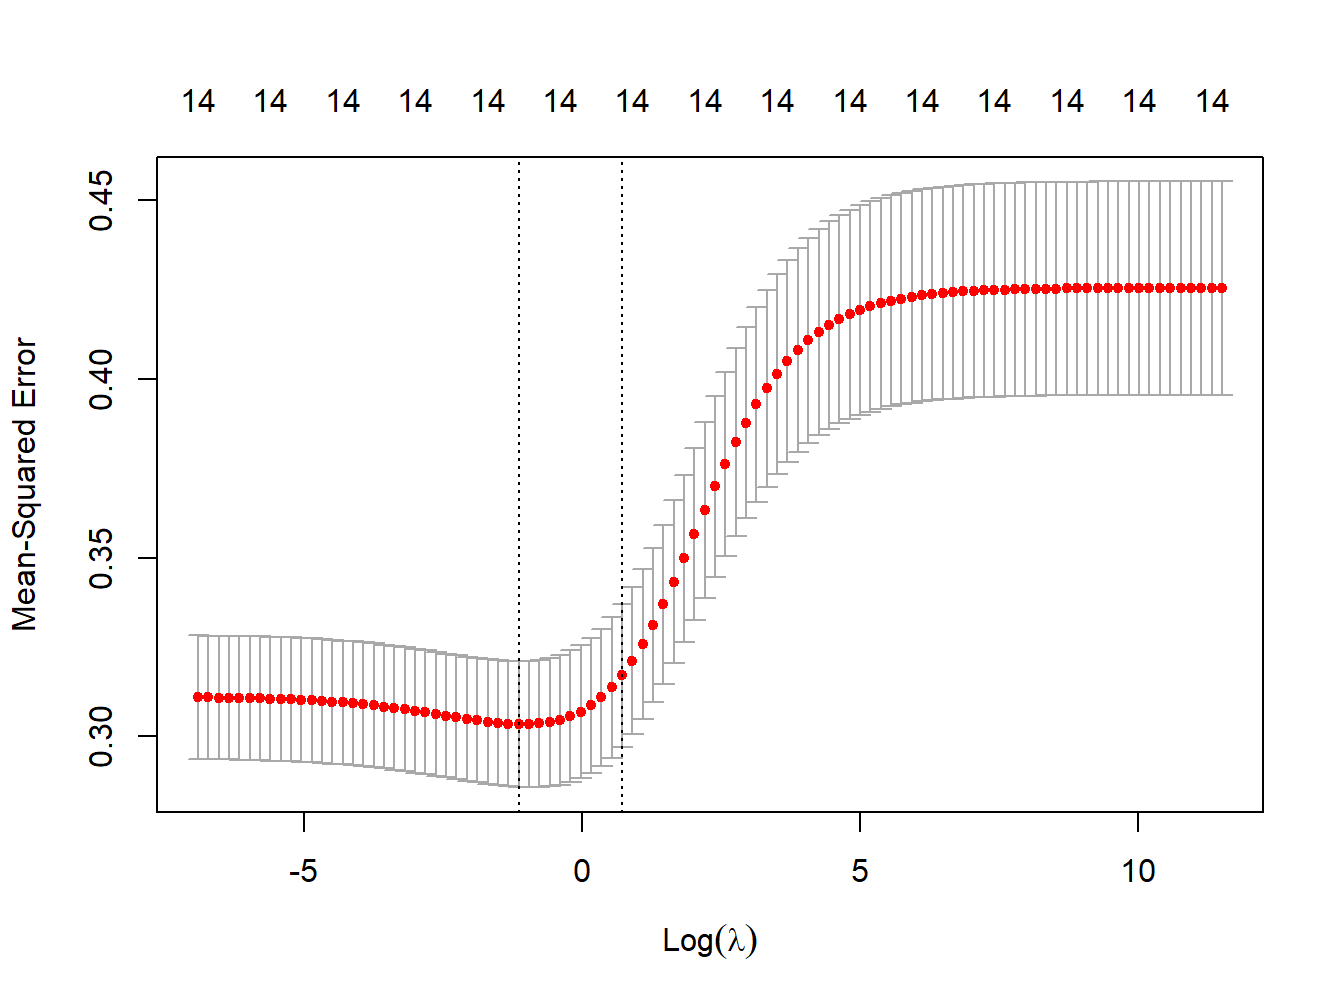
\includegraphics[width=0.8\linewidth]{bookdown-demo_files/figure-latex/figureridge-1} 

}

\caption{MSE vs lambda for ridge}\label{fig:figureridge}
\end{figure}

\begin{Shaded}
\begin{Highlighting}[]
\CommentTok{\# lowest lambda}
\NormalTok{lambda\_cv\_min }\OtherTok{\textless{}{-}}\NormalTok{ ridge\_cv}\SpecialCharTok{$}\NormalTok{lambda.min}
\NormalTok{lambda\_cv\_min}
\end{Highlighting}
\end{Shaded}

\begin{verbatim}
## [1] 0.3199267
\end{verbatim}

\begin{Shaded}
\begin{Highlighting}[]
\CommentTok{\# Best cross{-}validated lambda}
\NormalTok{lambda\_cv }\OtherTok{\textless{}{-}}\NormalTok{ ridge\_cv}\SpecialCharTok{$}\NormalTok{lambda}\FloatTok{.1}\NormalTok{se}
\NormalTok{lambda\_cv}
\end{Highlighting}
\end{Shaded}

\begin{verbatim}
## [1] 2.056512
\end{verbatim}

Another useful figure is the trajectory of coefficients at varying levels of \(\lambda\):

\begin{figure}[H]

{\centering 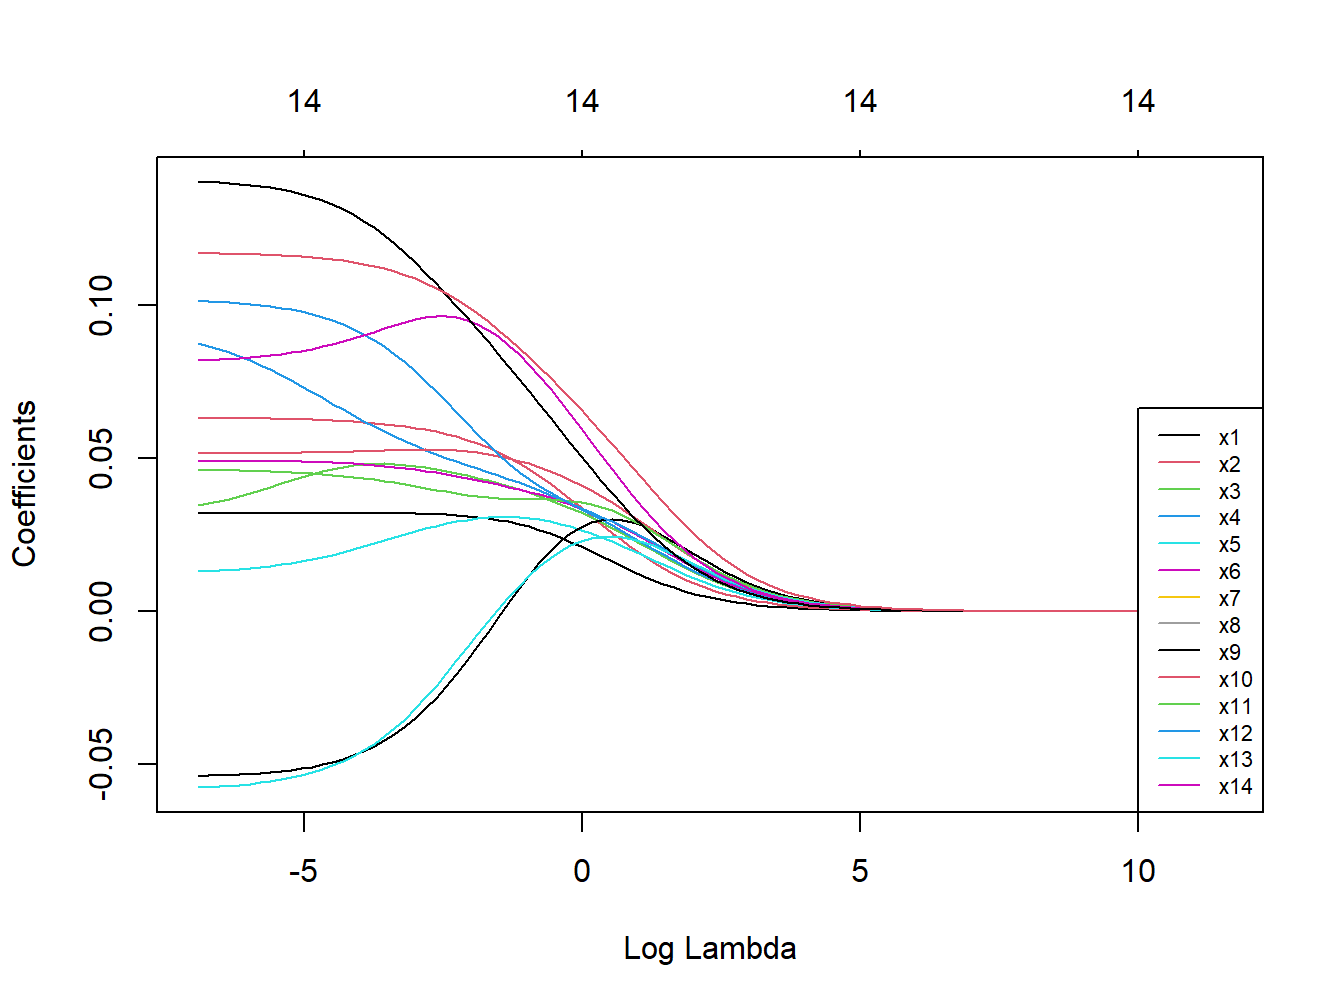
\includegraphics[width=0.8\linewidth]{bookdown-demo_files/figure-latex/figureridge2-1} 

}

\caption{coefficients trajectories for ridge}\label{fig:figureridge2}
\end{figure}

The starting values on the left of the figure are the ones from OLS estimation, and then we see how coefficients get shrinked at increasingly higher levels of \(\lambda\). Note that the shrinkage is operated on the entire model, and for this reason individual trajectories are not necessarily forced to decrease (here some coefficients become larger before getting shrinked). Also, from the numbers plotted on top of the figure, indicating the number of coefficients that are still included in the model, we can see that coefficients only tend asymptotically to 0 but are never really removed from the model.

Finally, we can summarize the results of our final model for the selected value of lambda:

\begin{Shaded}
\begin{Highlighting}[]
\NormalTok{model\_cv }\OtherTok{\textless{}{-}} \FunctionTok{glmnet}\NormalTok{(X, Y, }\AttributeTok{alpha =} \DecValTok{0}\NormalTok{, }\AttributeTok{lambda =}\NormalTok{ lambda\_cv, }\AttributeTok{standardize =} \ConstantTok{TRUE}\NormalTok{)}
\NormalTok{knitr}\SpecialCharTok{::}\FunctionTok{kable}\NormalTok{(}
 \FunctionTok{summary}\NormalTok{(model\_cv}\SpecialCharTok{$}\NormalTok{beta),}
  \AttributeTok{caption =} \StringTok{\textquotesingle{}Ridge\textquotesingle{}}
\NormalTok{)}
\end{Highlighting}
\end{Shaded}

\begin{table}

\caption{\label{tab:unnamed-chunk-16}Ridge}
\centering
\begin{tabular}[t]{r|r|r}
\hline
i & j & x\\
\hline
1 & 1 & 0.0147047\\
\hline
2 & 1 & 0.0231112\\
\hline
3 & 1 & 0.0254830\\
\hline
4 & 1 & 0.0263153\\
\hline
5 & 1 & 0.0214385\\
\hline
6 & 1 & 0.0276044\\
\hline
7 & 1 & 0.0299720\\
\hline
8 & 1 & 0.0334388\\
\hline
9 & 1 & 0.0315407\\
\hline
10 & 1 & 0.0277843\\
\hline
11 & 1 & 0.0242869\\
\hline
12 & 1 & 0.0420859\\
\hline
13 & 1 & 0.0348748\\
\hline
14 & 1 & 0.0508906\\
\hline
\end{tabular}
\end{table}

These results can provide some useful information but are of little use in our context. For example, we know from our VIF analysis that the coefficients for \(X_{12}\) and \(X_{13}\) are affected by high collinearity, but we would like to understand whether a real association exists for both exposures or whether one of the 2 is driving the cluster. To do so, we might prefer to operate some sort of variable selection, constructing a penalty so that non-influential covariates can be set to 0 (and therefore removed). This is what LASSO does.

\hypertarget{lasso}{%
\subsection{LASSO}\label{lasso}}

Lasso, standing for Least Absolute Shrinkage and Selection Operator, also adds a penalty to the loss function of OLS. However, instead of adding a penalty that penalizes sum of squared residuals (L2 penalty), Lasso penalizes the sum of their absolute values (L1 penalty). As a results, for high values of \(\lambda\), many coefficients are exactly zeroed under lasso, which is never the case in ridge regression (where 0s are the extreme case as \(\lambda\rightarrow\infty\)). Specifically, the Lasso estimator can be written as
\textbackslash end\{itemize\}
\[L_{lasso}(\hat{\beta})=\sum_{i=1}^n(y_i-x_i'\hat{\beta})^2+\lambda\sum_{j=1}^m|\hat{\beta}_j|\]
\textbackslash end\{frame\}

As before, let's turn to our illustrative example to understand properties and interpretation. The procedure in R is exactly the same, with the only difference that the parameter \(\alpha\) is set to 1. First, let's identify the optimal value of \(\lambda\) using the cross validation procedure,

\begin{Shaded}
\begin{Highlighting}[]
\NormalTok{lasso\_cv }\OtherTok{\textless{}{-}} \FunctionTok{cv.glmnet}\NormalTok{(X, Y, }\AttributeTok{alpha =} \DecValTok{1}\NormalTok{, }\AttributeTok{lambda =}\NormalTok{ lambdas\_to\_try,}
                      \AttributeTok{standardize =} \ConstantTok{TRUE}\NormalTok{, }\AttributeTok{nfolds =} \DecValTok{10}\NormalTok{)}
\end{Highlighting}
\end{Shaded}

\begin{figure}[H]

{\centering 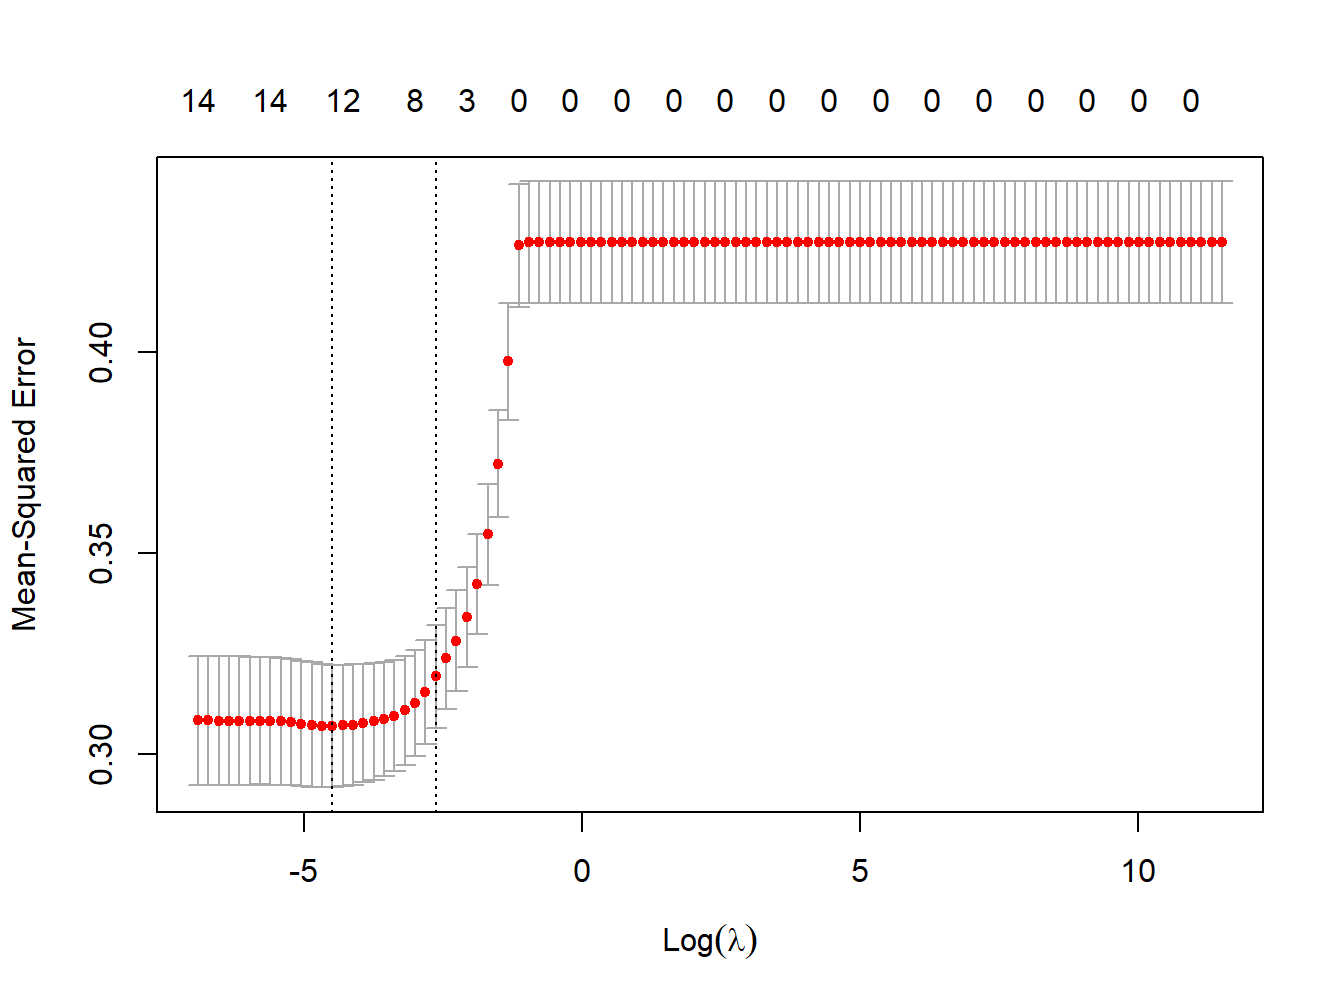
\includegraphics[width=0.8\linewidth]{bookdown-demo_files/figure-latex/figurelasso-1} 

}

\caption{MSE vs lambda for lasso}\label{fig:figurelasso}
\end{figure}

\begin{Shaded}
\begin{Highlighting}[]
\CommentTok{\# lowest lambda}
\NormalTok{lambda\_cv\_min\_lasso }\OtherTok{\textless{}{-}}\NormalTok{ lasso\_cv}\SpecialCharTok{$}\NormalTok{lambda.min}
\NormalTok{lambda\_cv\_min\_lasso}
\end{Highlighting}
\end{Shaded}

\begin{verbatim}
## [1] 0.01123324
\end{verbatim}

\begin{Shaded}
\begin{Highlighting}[]
\CommentTok{\# Best cross{-}validated lambda}
\NormalTok{lambda\_cv\_lasso }\OtherTok{\textless{}{-}}\NormalTok{ lasso\_cv}\SpecialCharTok{$}\NormalTok{lambda}\FloatTok{.1}\NormalTok{se}
\NormalTok{lambda\_cv\_lasso}
\end{Highlighting}
\end{Shaded}

\begin{verbatim}
## [1] 0.07220809
\end{verbatim}

and then plot the coefficients trajectories.

\begin{figure}[H]

{\centering 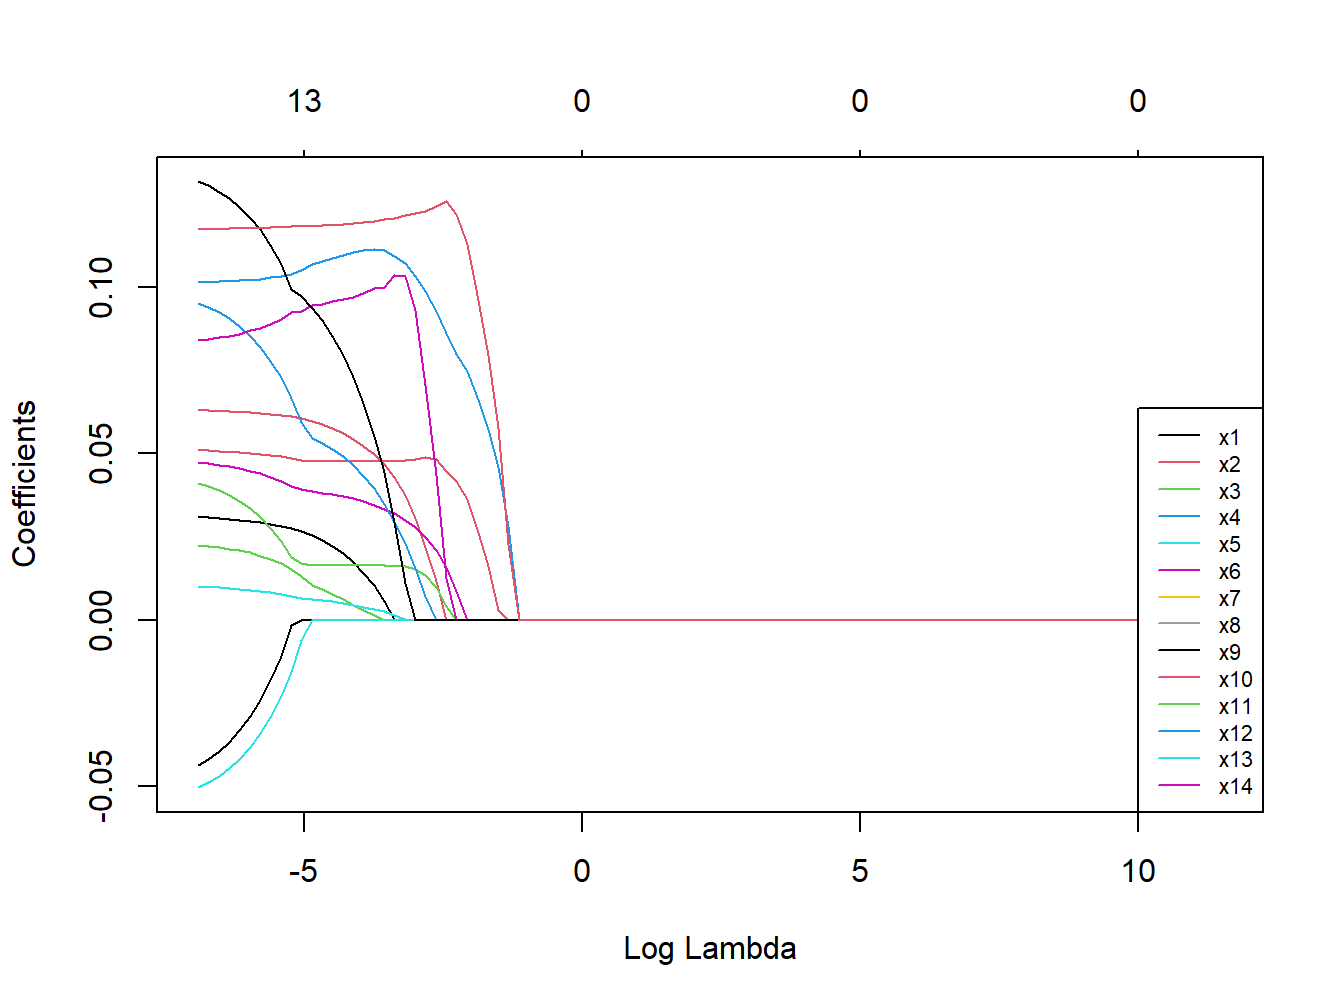
\includegraphics[width=0.8\linewidth]{bookdown-demo_files/figure-latex/figurelasso2-1} 

}

\caption{coefficients trajectories for lasso}\label{fig:figurelasso2}
\end{figure}

We see that, differently from what observed in Ridge regression, coefficients are shrinked to a point where they exactly equal 0, and are therefore excluded from the model. The numbers on top of Figure 3.4 show how many exposures are left in the model at higher levels of \(\lambda\). Finally, let's take a look at the results of the optimal selected model.

\begin{Shaded}
\begin{Highlighting}[]
\NormalTok{model\_cv\_lasso }\OtherTok{\textless{}{-}} \FunctionTok{glmnet}\NormalTok{(X, Y, }\AttributeTok{alpha =} \DecValTok{1}\NormalTok{, }\AttributeTok{lambda =}\NormalTok{ lambda\_cv\_lasso, }\AttributeTok{standardize =} \ConstantTok{TRUE}\NormalTok{)}
\NormalTok{knitr}\SpecialCharTok{::}\FunctionTok{kable}\NormalTok{(}
 \FunctionTok{summary}\NormalTok{(model\_cv\_lasso}\SpecialCharTok{$}\NormalTok{beta),}
  \AttributeTok{caption =} \StringTok{\textquotesingle{}Lasso\textquotesingle{}}
\NormalTok{)}
\end{Highlighting}
\end{Shaded}

\begin{table}

\caption{\label{tab:unnamed-chunk-17}Lasso}
\centering
\begin{tabular}[t]{r|r|r}
\hline
i & j & x\\
\hline
2 & 1 & 0.0115952\\
\hline
4 & 1 & 0.0930313\\
\hline
6 & 1 & 0.0210787\\
\hline
8 & 1 & 0.0483009\\
\hline
9 & 1 & 0.0100253\\
\hline
12 & 1 & 0.0436241\\
\hline
14 & 1 & 0.1242974\\
\hline
\end{tabular}
\end{table}

The final model selects only 6 covariates, while all other 8 drop to 0. If we look at our 2 established groups of correlated exposures, \(X_4\) and \(X_{12}\) are selected, while the others are left out. In general, Lasso's results may be very sensitive to weak associations, dropping coefficients that are not actually 0. Lasso can set some coefficients to zero, thus performing variable selection, while ridge regression cannot. The two methods solve multicollinearity differently: in ridge regression, the coefficients of correlated predictors are similar, while in lasso, one of the correlated predictors has a larger coefficient, while the rest are (nearly) zeroed. Lasso tends to do well if there are a small number of significant parameters and the others are close to zero (that is - when only a few predictors actually influence the response). Ridge works well if there are many large parameters of about the same value (that is - when most predictors impact the response).

\hypertarget{elastic-net}{%
\subsection{Elastic net}\label{elastic-net}}

Rather than debating which model is better, we can directly use Elastic Net, which has been designed as a compromise between Lasso and Ridge, attempting to overcome their limitations and performing variable selection in a less rigid way than Lasso. Elastic Net combines the penalties of ridge regression and Lasso, aiming at minimizing the following loss function

\[L_{enet}(\hat{\beta})=\frac{\sum_{i=1}^n(y_i-x_i'\hat{\beta})^2}{2n}+\lambda\left(\frac{1-\alpha}{2}\sum_{j=1}^m\hat{\beta}_j^2+\alpha\sum_{j=1}^m|\hat{\beta}_j|\right)\]

where \(\alpha\) is the mixing parameter between ridge (\(\alpha\)=0) and lasso (\(\alpha\)=1). How this loss function is derived, given the ridge and lasso ones, is described in \citet{zou2005regularization}. Procedures to simultaneously tune both \(\alpha\) and \(\lambda\) to retrieve the optimal combinations are available and developed in the R package \texttt{caret}. For simplicity we will here stick on \texttt{glmnet}, which requires pre-defining a value for \(\alpha\). One can of course fit several models and compare them with common indexes such as AIC or BIC. To ensure some variable selection, we may for example choose a value of \(\lambda\) like 0.7, closer to Lasso than to Ridge. Let's fit an Elastic Net model, with \(\alpha=0.7\) in our example. First, we need to select the optimal value of \(\lambda\):

\begin{Shaded}
\begin{Highlighting}[]
\NormalTok{enet\_cv }\OtherTok{\textless{}{-}} \FunctionTok{cv.glmnet}\NormalTok{(X, Y, }\AttributeTok{alpha =} \FloatTok{0.7}\NormalTok{, }\AttributeTok{lambda =}\NormalTok{ lambdas\_to\_try,}
                     \AttributeTok{standardize =} \ConstantTok{TRUE}\NormalTok{, }\AttributeTok{nfolds =} \DecValTok{10}\NormalTok{)}
\end{Highlighting}
\end{Shaded}

\begin{figure}[H]

{\centering 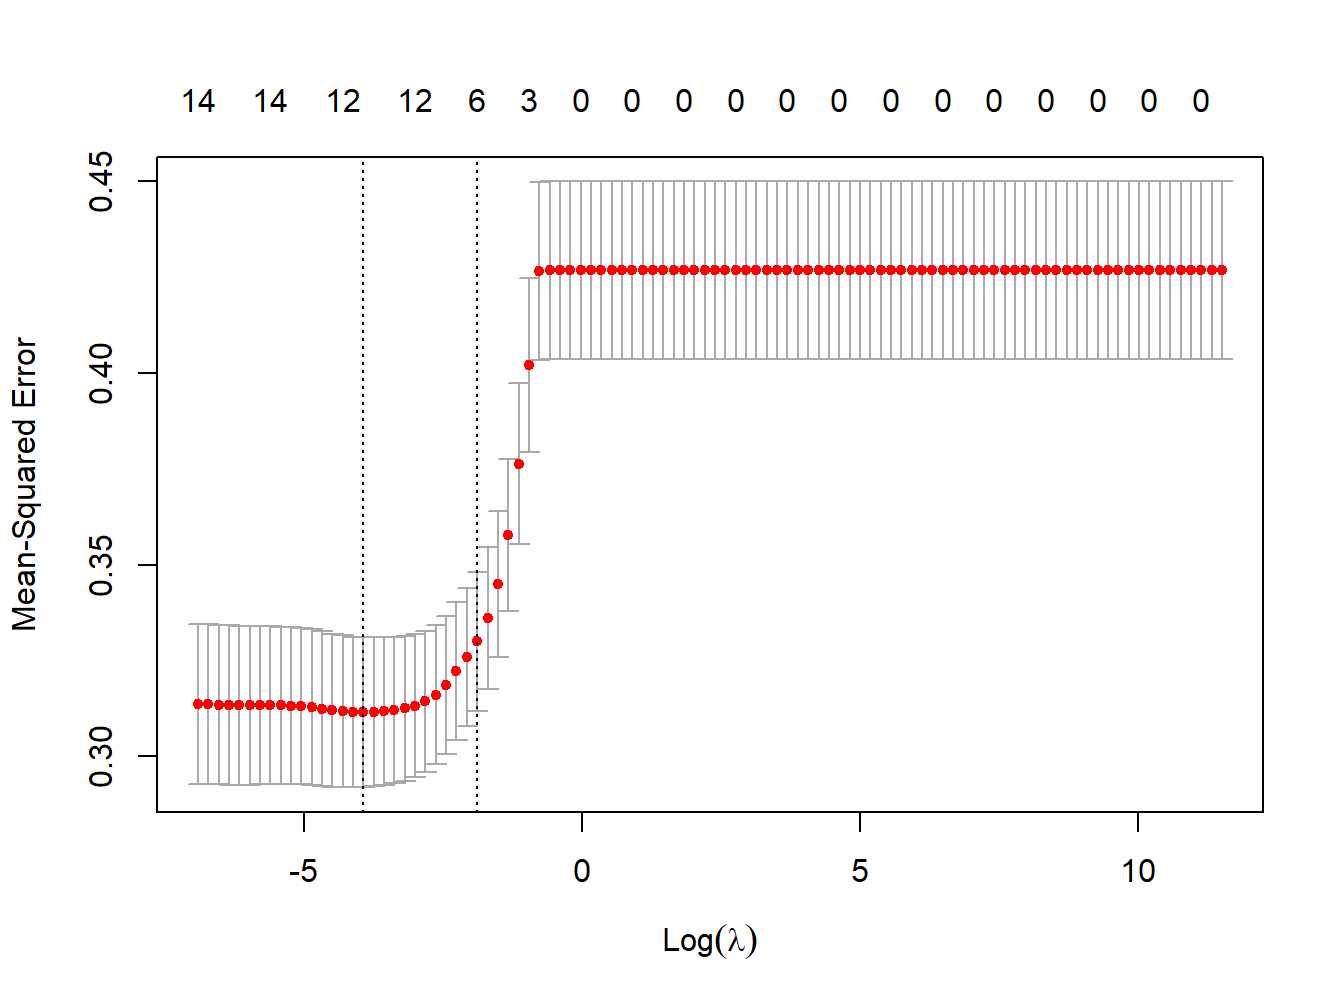
\includegraphics[width=0.8\linewidth]{bookdown-demo_files/figure-latex/figureenet-1} 

}

\caption{MSE vs lambda for elastic net}\label{fig:figureenet}
\end{figure}

\begin{Shaded}
\begin{Highlighting}[]
\NormalTok{lambda\_cv\_min\_enet }\OtherTok{\textless{}{-}}\NormalTok{ enet\_cv}\SpecialCharTok{$}\NormalTok{lambda.min}
\NormalTok{lambda\_cv\_min\_enet}
\end{Highlighting}
\end{Shaded}

\begin{verbatim}
## [1] 0.01963041
\end{verbatim}

\begin{Shaded}
\begin{Highlighting}[]
\CommentTok{\# Best cross{-}validated lambda}
\NormalTok{lambda\_cv\_enet }\OtherTok{\textless{}{-}}\NormalTok{ enet\_cv}\SpecialCharTok{$}\NormalTok{lambda}\FloatTok{.1}\NormalTok{se}
\NormalTok{lambda\_cv\_enet}
\end{Highlighting}
\end{Shaded}

\begin{verbatim}
## [1] 0.1519911
\end{verbatim}

and plot the coefficients' trajectories.

\begin{figure}[H]

{\centering 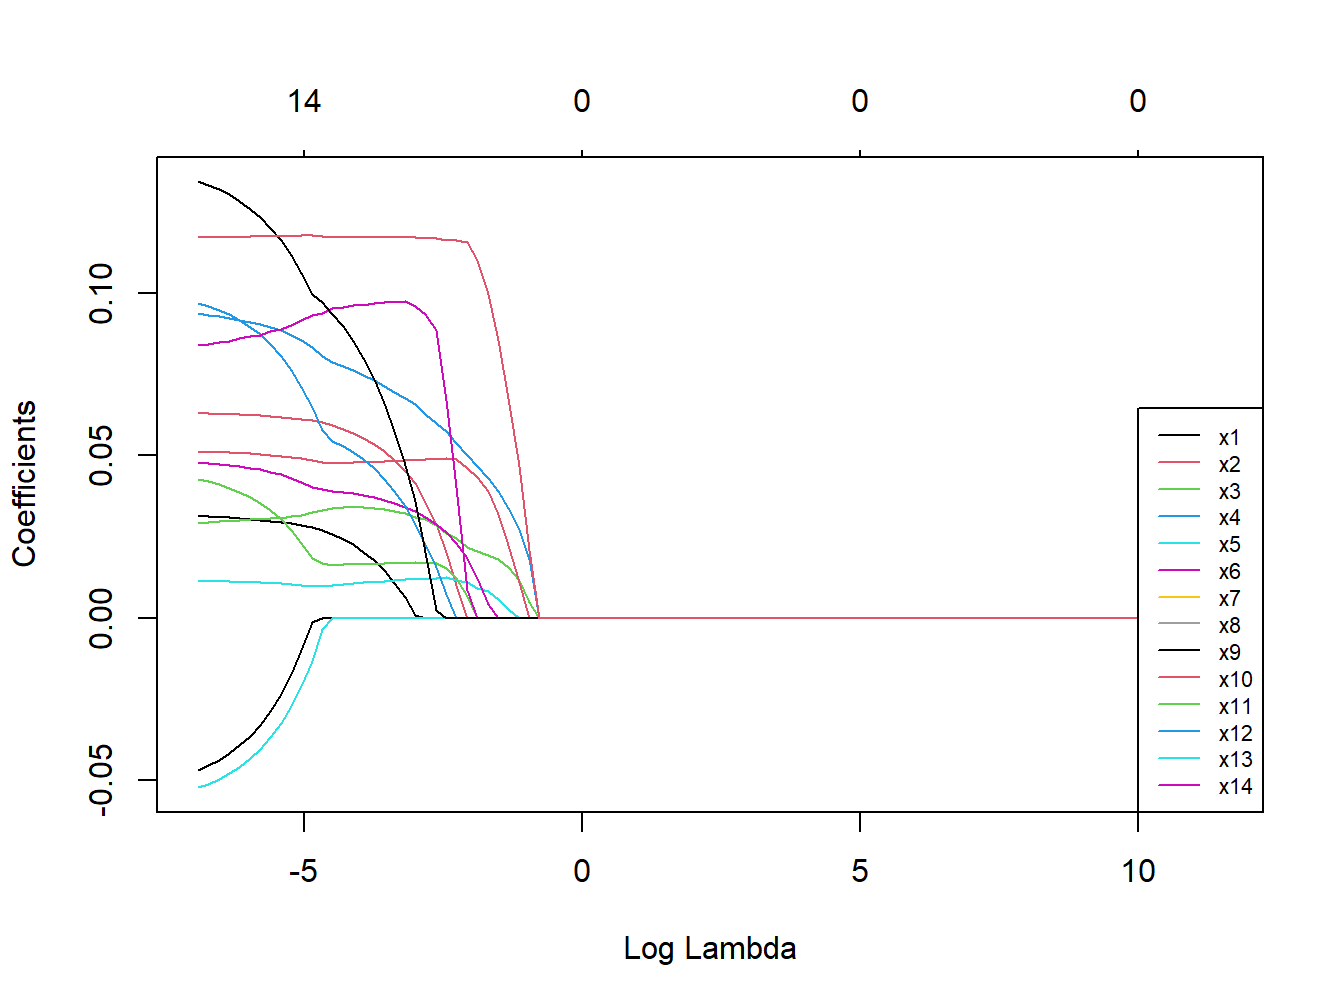
\includegraphics[width=0.8\linewidth]{bookdown-demo_files/figure-latex/figureenet2-1} 

}

\caption{coefficients trajectories for elastic net}\label{fig:figureenet2}
\end{figure}

We see that coefficients are shrinked to a point where they exactly equal 0, and therefore excluded from the model, but that this happens more conservatively as compared to Lasso (as documented from the numbers on top). Let's take a look at the results of the optimal selected model.

\begin{Shaded}
\begin{Highlighting}[]
\NormalTok{model\_cv\_enet }\OtherTok{\textless{}{-}} \FunctionTok{glmnet}\NormalTok{(X, Y, }\AttributeTok{alpha =} \FloatTok{0.7}\NormalTok{, }\AttributeTok{lambda =}\NormalTok{ lambda\_cv\_enet, }\AttributeTok{standardize =} \ConstantTok{TRUE}\NormalTok{)}
\NormalTok{knitr}\SpecialCharTok{::}\FunctionTok{kable}\NormalTok{(}

\FunctionTok{summary}\NormalTok{(model\_cv\_enet}\SpecialCharTok{$}\NormalTok{beta),}
  \AttributeTok{caption =} \StringTok{\textquotesingle{}Lasso\textquotesingle{}}
\NormalTok{)}
\end{Highlighting}
\end{Shaded}

\begin{table}

\caption{\label{tab:unnamed-chunk-18}Lasso}
\centering
\begin{tabular}[t]{r|r|r}
\hline
i & j & x\\
\hline
3 & 1 & 0.0209672\\
\hline
4 & 1 & 0.0465784\\
\hline
5 & 1 & 0.0090842\\
\hline
6 & 1 & 0.0123642\\
\hline
8 & 1 & 0.0430287\\
\hline
14 & 1 & 0.1098168\\
\hline
\end{tabular}
\end{table}

As expected, less covariates are dropped to 0. Unfortunately, however, all components of the group of correlated covariates \(X_3-X_5\) remain in the model, and we are not able to identify the key actor of that group. Before getting deeper into the discussion of these results, however, it is useful to incorporate the potential confounders available in the data. Including confounders can be done by specifying them in the model as we do in a regular OLS model. However, we may want them to be involved in the selection process. To such end, the best way is to include them in the matrix of covariates to be penalized, but inform the CV procedure that you don't want their coefficients to be modified. The following chunk of code will do that:

\begin{Shaded}
\begin{Highlighting}[]
\NormalTok{X}\OtherTok{\textless{}{-}}\FunctionTok{as.matrix}\NormalTok{(data2[,}\DecValTok{3}\SpecialCharTok{:}\DecValTok{19}\NormalTok{])}

\NormalTok{enet\_cv\_adj }\OtherTok{\textless{}{-}} \FunctionTok{cv.glmnet}\NormalTok{(X, Y, }\AttributeTok{alpha =} \FloatTok{0.6}\NormalTok{, }\AttributeTok{lambda =}\NormalTok{ lambdas\_to\_try,}
                     \AttributeTok{standardize =} \ConstantTok{TRUE}\NormalTok{, }\AttributeTok{nfolds =} \DecValTok{10}\NormalTok{, }\AttributeTok{penalty.factor=}\FunctionTok{c}\NormalTok{(}\FunctionTok{rep}\NormalTok{(}\DecValTok{1}\NormalTok{,}\FunctionTok{ncol}\NormalTok{(X) }\SpecialCharTok{{-}} \DecValTok{3}\NormalTok{),}\DecValTok{0}\NormalTok{,}\DecValTok{0}\NormalTok{,}\DecValTok{0}\NormalTok{))}
\end{Highlighting}
\end{Shaded}

\begin{figure}[H]

{\centering 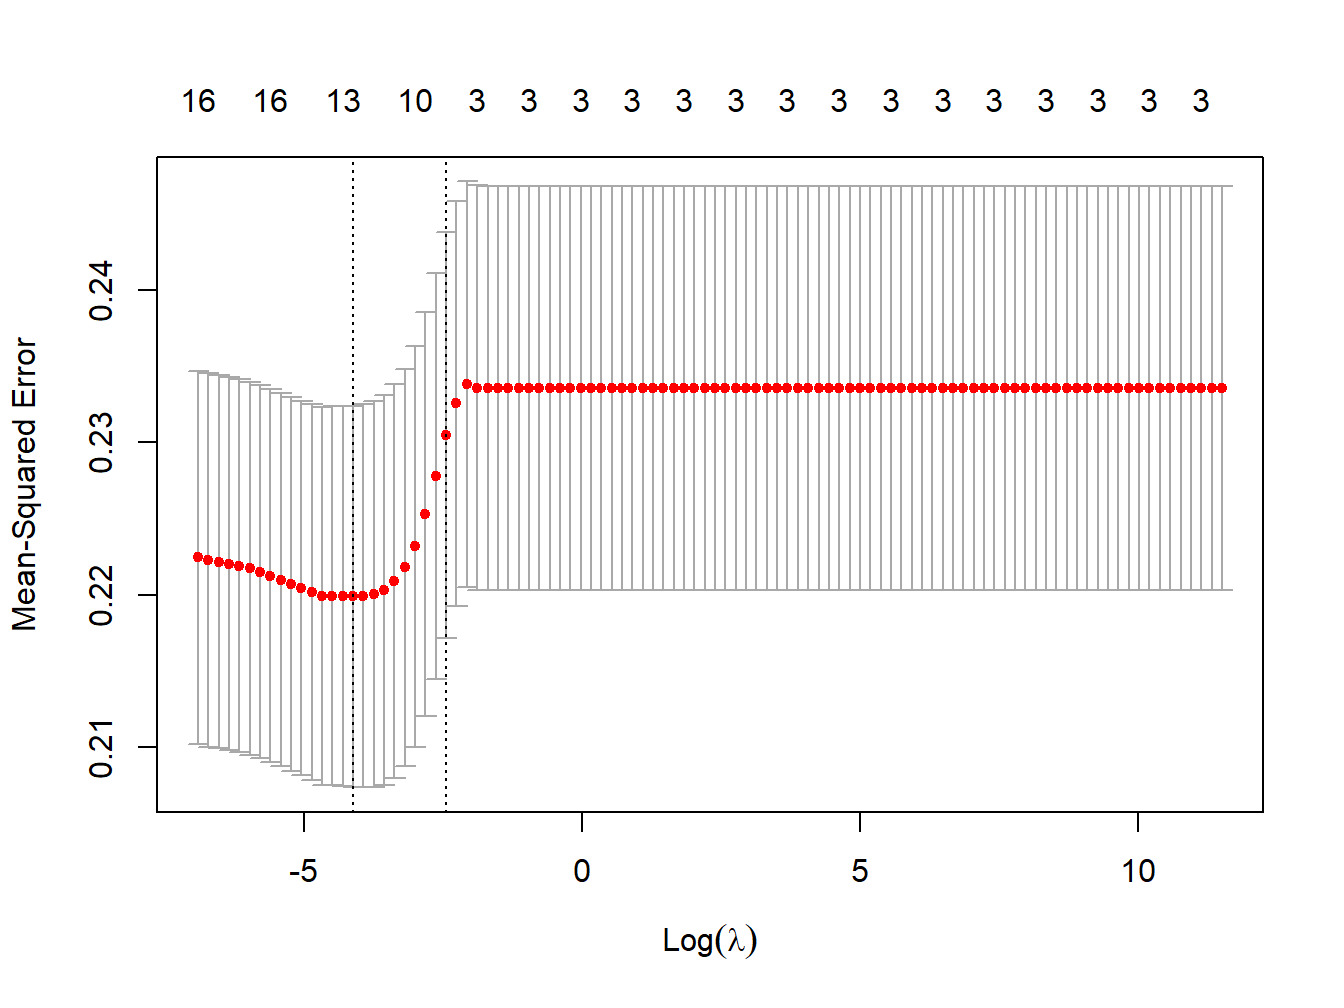
\includegraphics[width=0.8\linewidth]{bookdown-demo_files/figure-latex/figureenetadjasdfasdf-1} 

}

\caption{MSE vs lambda for elastic net, adjusted for confounders}\label{fig:figureenetadjasdfasdf}
\end{figure}

\begin{Shaded}
\begin{Highlighting}[]
\NormalTok{lambda\_cv\_min\_enet\_adj }\OtherTok{\textless{}{-}}\NormalTok{ enet\_cv\_adj}\SpecialCharTok{$}\NormalTok{lambda.min}
\NormalTok{lambda\_cv\_min\_enet\_adj}
\end{Highlighting}
\end{Shaded}

\begin{verbatim}
## [1] 0.01629751
\end{verbatim}

\begin{Shaded}
\begin{Highlighting}[]
\CommentTok{\# Best cross{-}validated lambda}
\NormalTok{lambda\_cv\_enet\_adj }\OtherTok{\textless{}{-}}\NormalTok{ enet\_cv\_adj}\SpecialCharTok{$}\NormalTok{lambda}\FloatTok{.1}\NormalTok{se}
\NormalTok{lambda\_cv\_enet\_adj}
\end{Highlighting}
\end{Shaded}

\begin{verbatim}
## [1] 0.0869749
\end{verbatim}

Note that, regardless of how large \(\lambda\) will be, the three confounders will remain non-penalized in the model, as documented from the numbers on top. Here the final results:

\begin{Shaded}
\begin{Highlighting}[]
\NormalTok{model\_cv\_enet\_adj }\OtherTok{\textless{}{-}} \FunctionTok{glmnet}\NormalTok{(X, Y, }\AttributeTok{alpha =} \FloatTok{0.6}\NormalTok{, }\AttributeTok{lambda =}\NormalTok{ lambda\_cv\_enet, }\AttributeTok{standardize =} \ConstantTok{TRUE}\NormalTok{,}\AttributeTok{penalty.factor=}\FunctionTok{c}\NormalTok{(}\FunctionTok{rep}\NormalTok{(}\DecValTok{1}\NormalTok{,}\FunctionTok{ncol}\NormalTok{(X) }\SpecialCharTok{{-}} \DecValTok{3}\NormalTok{),}\DecValTok{0}\NormalTok{,}\DecValTok{0}\NormalTok{,}\DecValTok{0}\NormalTok{))}
\NormalTok{knitr}\SpecialCharTok{::}\FunctionTok{kable}\NormalTok{(}

\FunctionTok{summary}\NormalTok{(model\_cv\_enet\_adj}\SpecialCharTok{$}\NormalTok{beta),}
  \AttributeTok{caption =} \StringTok{\textquotesingle{}Lasso, adjusted\textquotesingle{}}
\NormalTok{)}
\end{Highlighting}
\end{Shaded}

\begin{table}

\caption{\label{tab:unnamed-chunk-19}Lasso, adjusted}
\centering
\begin{tabular}[t]{r|r|r}
\hline
i & j & x\\
\hline
15 & 1 & -0.0101247\\
\hline
16 & 1 & 0.0119696\\
\hline
17 & 1 & -0.6454254\\
\hline
\end{tabular}
\end{table}

In addition to the 3 confounders (now named \(X_{15}-X_{17}\)) only 4 covariates did not drop to 0. Interestingly, we are now selecting none of the 3 covariates we wanted to distinguish. Results seem to agree with multiple regression in indicating \(X_6\) and \(X_{12}\) as the main predictors of the outcome.

\hypertarget{additional-notes}{%
\subsection{Additional notes}\label{additional-notes}}

We have covered the basic theory of penalized regression techniques (also referred to with other common terminology such as shrinkage procedures, or regularization processes). Before moving to the presentation of two examples of application of these techniques in environmental epidemiology, let's mention some additional details.

\begin{itemize}
\tightlist
\item
  Replicate results in classical OLS
\end{itemize}

When Elastic Net is used to describe associations in population-based studies, it is common practice to also present a final linear regression model that only includes those predictors that were selected from the penalized approach. This model will ensure better interpretation of the coefficients, and hopefully not be subject anymore to issues of collinearity that the selection should have addressed. Here are the results from such model in our illustrative example, based on covariates selected by the final adjusted elastic net model.

Dependent variable:

y

(1)

(2)

x1

0.058* (-0.007, 0.123)

x2

0.018 (-0.043, 0.080)

x3

-0.030 (-0.232, 0.173)

x4

0.053 (-0.170, 0.275)

x5

0.004 (-0.080, 0.088)

x6

0.085*** (0.031, 0.139)

0.060** (0.001, 0.119)

x7

-0.031 (-0.153, 0.091)

x8

0.017 (-0.063, 0.097)

x9

0.015 (-0.081, 0.111)

0.025 (-0.090, 0.140)

x10

0.085** (0.019, 0.152)

0.052 (-0.039, 0.144)

x11

0.049 (-0.052, 0.151)

x12

0.224*** (0.074, 0.374)

0.222 (-0.071, 0.515)

x13

-0.083 (-0.382, 0.216)

x14

0.054 (-0.047, 0.154)

z1

0.003 (-0.023, 0.030)

0.006 (-0.021, 0.032)

z2

0.009*** (0.006, 0.011)

0.006*** (0.003, 0.010)

z3

-0.617*** (-0.700, -0.534)

-0.609*** (-0.696, -0.522)

Constant

3.476*** (3.272, 3.680)

3.265*** (2.800, 3.730)

Observations

500

500

Note:

\emph{p\textless0.1; \textbf{p\textless0.05; }}p\textless0.01

\begin{itemize}
\tightlist
\item
  Grouped Lasso
\end{itemize}

In some settings, the predictors belong to pre-defined groups, or we might have observed well-defined subgroups of exposures from our PCA. In this situation one may want to shrink and select together the members of a given group, which can be achieved with grouped Lasso. The next section will provide alternative regression approaches where preliminary grouping information can be used to address some limitations of standard regression.

\begin{itemize}
\tightlist
\item
  Time-to-event outcomes
\end{itemize}

Recent developments allow fitting Elastic Net with time-to-event outcomes, within the context of a regularized Cox regression model. Given the popularity of this method in epidemiology it is reasonable to expect that this approach will become more popular in the context of environmental mixture since (as we will see in next sections) methods that were built ad-hoc do not always account for these types of outcomes. A first R package was develop in 2011 (\texttt{coxnet}), fully documented \href{https://cran.r-project.org/web/packages/glmnet/vignettes/Coxnet.pdf}{here}, and those algorithms for right-censored data have also been included in the most recent version of \texttt{glmnet}

\begin{itemize}
\tightlist
\item
  Non-linear associations
\end{itemize}

An implicit assumption we have made so far is that each covariate included in the model has a linear (or log-linear) effect on the outcome of interest. We know that this is often not true (several environmental exposures, for example, have some kind of plateau effect) and we might want to be able to incorporate non-linearities in our analyses. While classical regression can flexibly allow incorporating non-linearities by means of techniques such as restricted cubic splines, this is not of straightforward application in penalized regression. In complex settings where strong departures from linearity are observed in preliminary linear regressions, one should probably consider more flexible techniques such as BKMR (Section 5).

\hypertarget{elastic-net-and-environmental-mixtures}{%
\subsection{Elastic Net and environmental mixtures}\label{elastic-net-and-environmental-mixtures}}

Using Elastic Net to evaluate the association between a mixture of environemtanl exposures and a health outcome is becoming increasingly popular. A nice and rigorous application of the method can be found in \citet{lenters2016prenatal}, evaluating co-exposure to 16 chemicals as they relate to birth weight in 1250 infants. Here the correlation plot from the manuscript,

/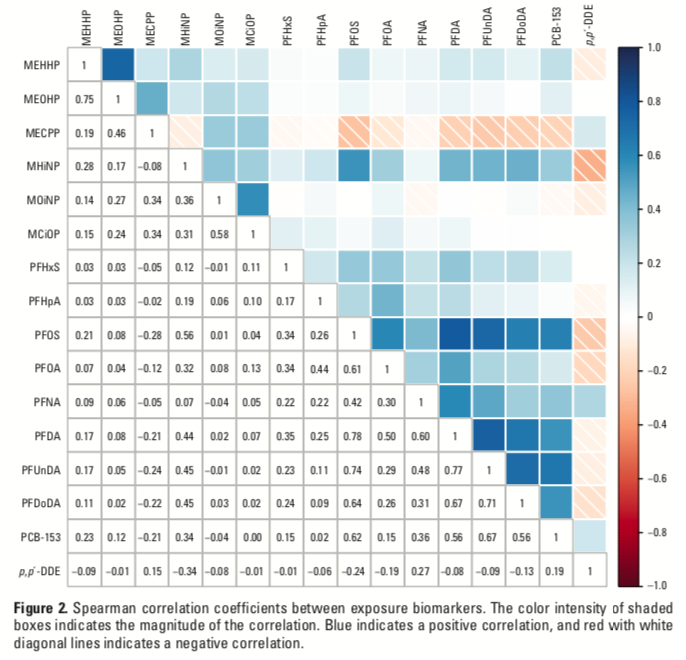
\includegraphics{images/corrplot.png}

and here results presenting, respectively, the Elastic Net model, and the final OLS only including selected covariates.
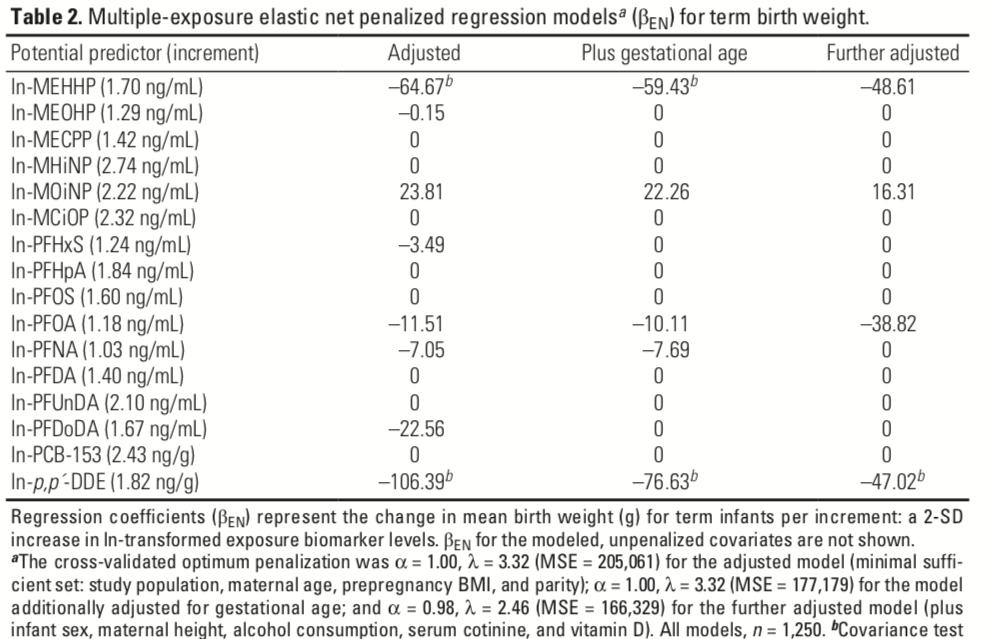
\includegraphics{images/table2.png}

\begin{figure}
\centering
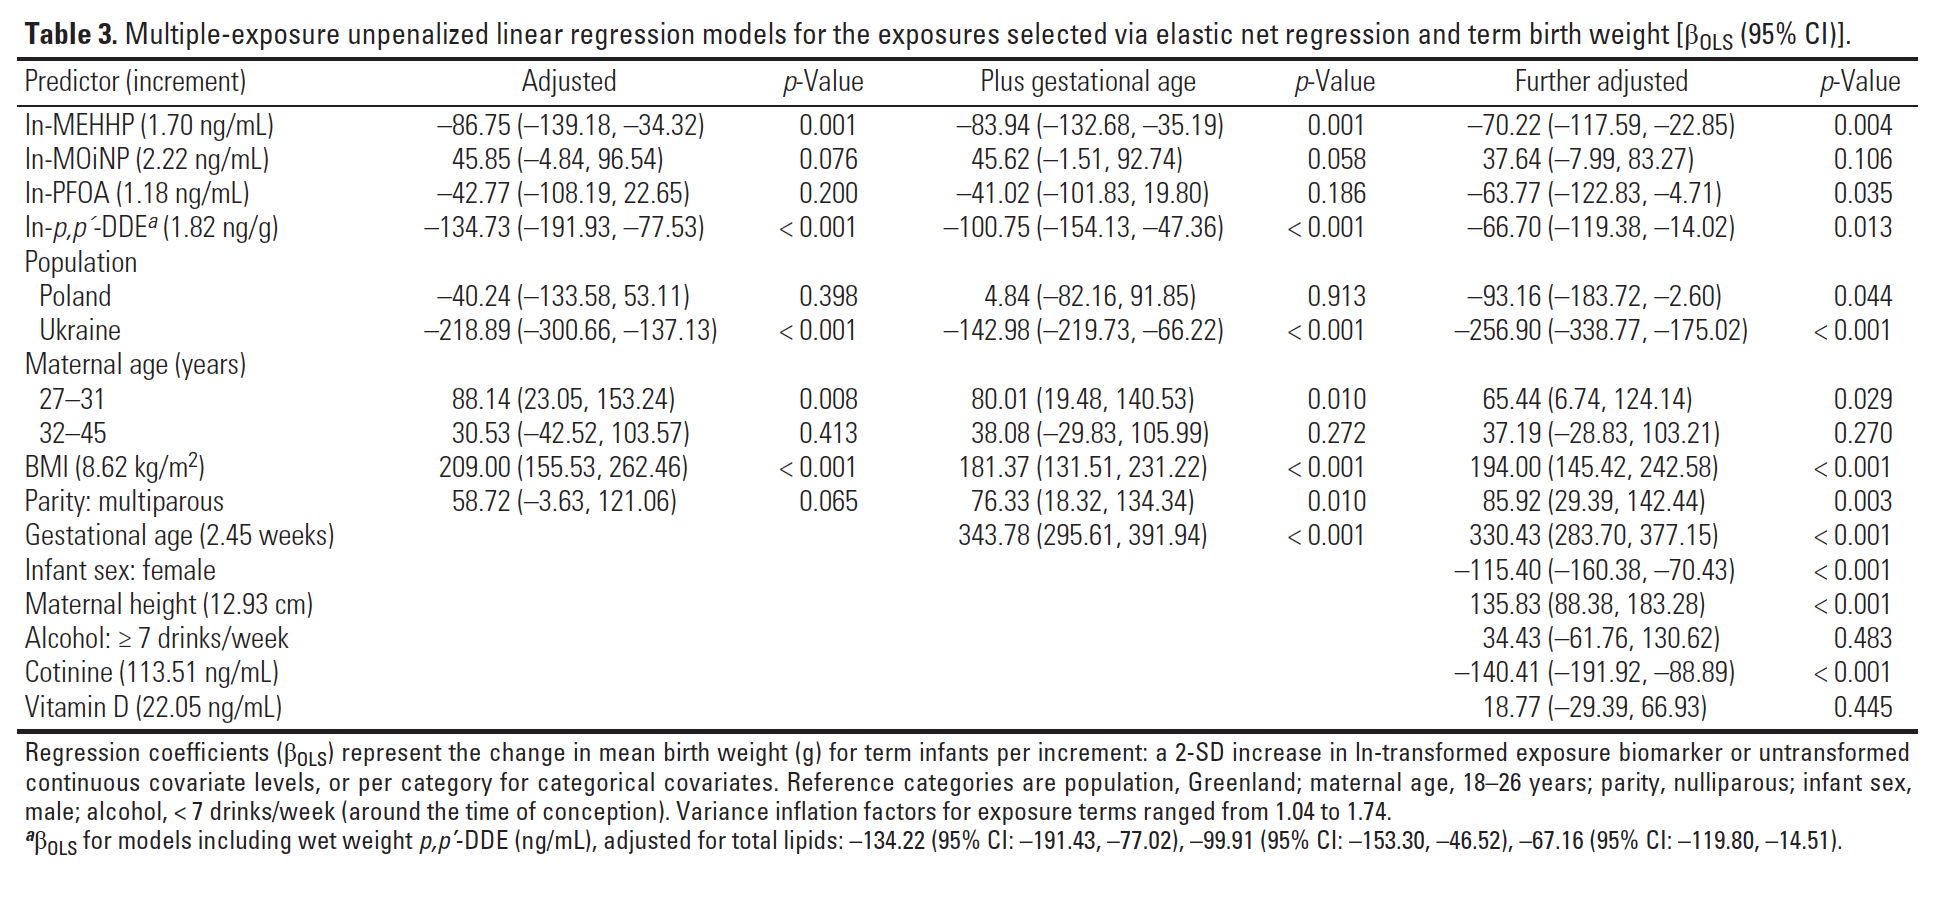
\includegraphics{images/table3.png}
\caption{Table 3 from Lenters et al.}
\end{figure}

Another application that thoroughly report methods presentation, stating all assumptions and clearly discussing the results, can be seen in \citet{vriens2017neonatal}, evaluating environmental pollutants and placental mitochondrial DNA content in infants. This is the starting correlation plot reported in the paper:

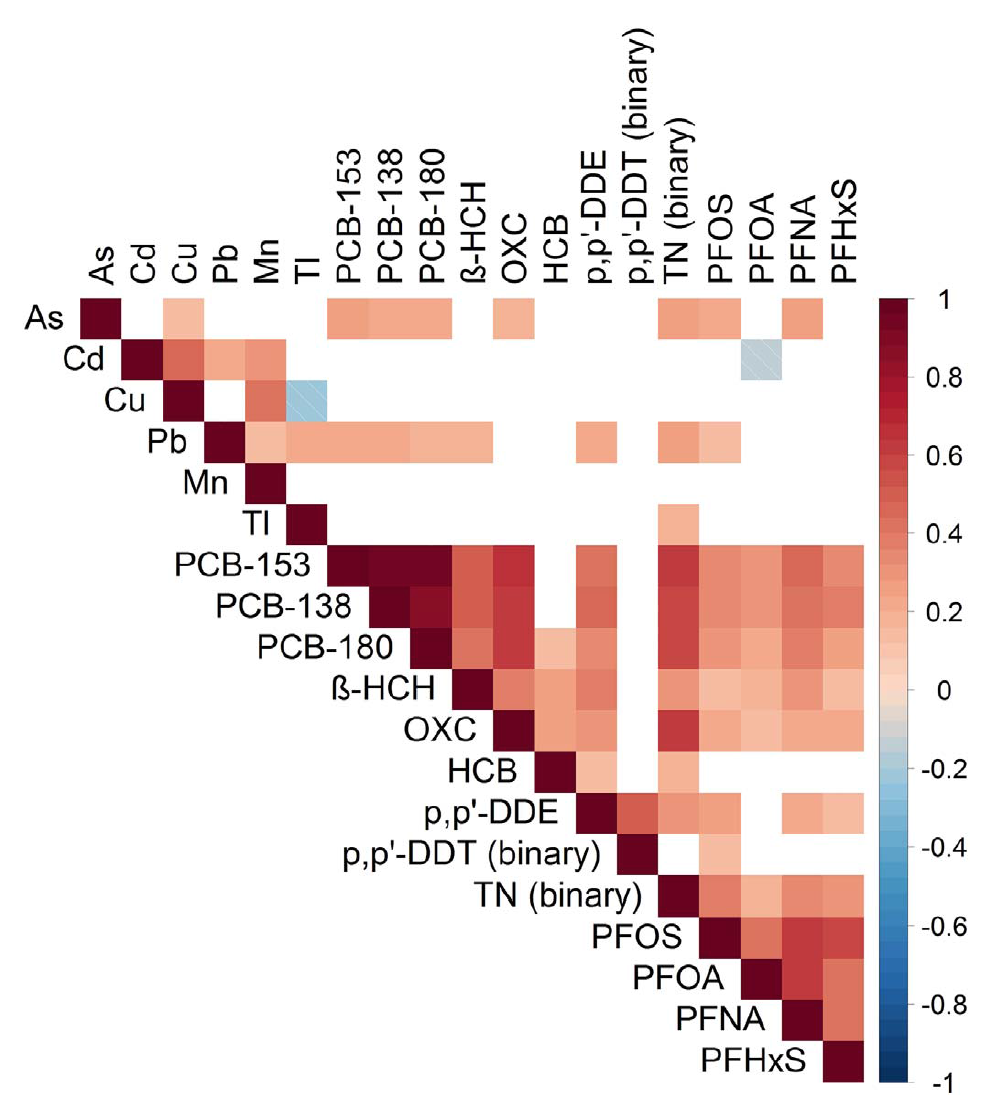
\includegraphics{images/corrplot2.png}
Several detailed figures are used to present results providing the reader with all necessary tools to understand associations and provide clear interpretation.

\begin{figure}
\centering
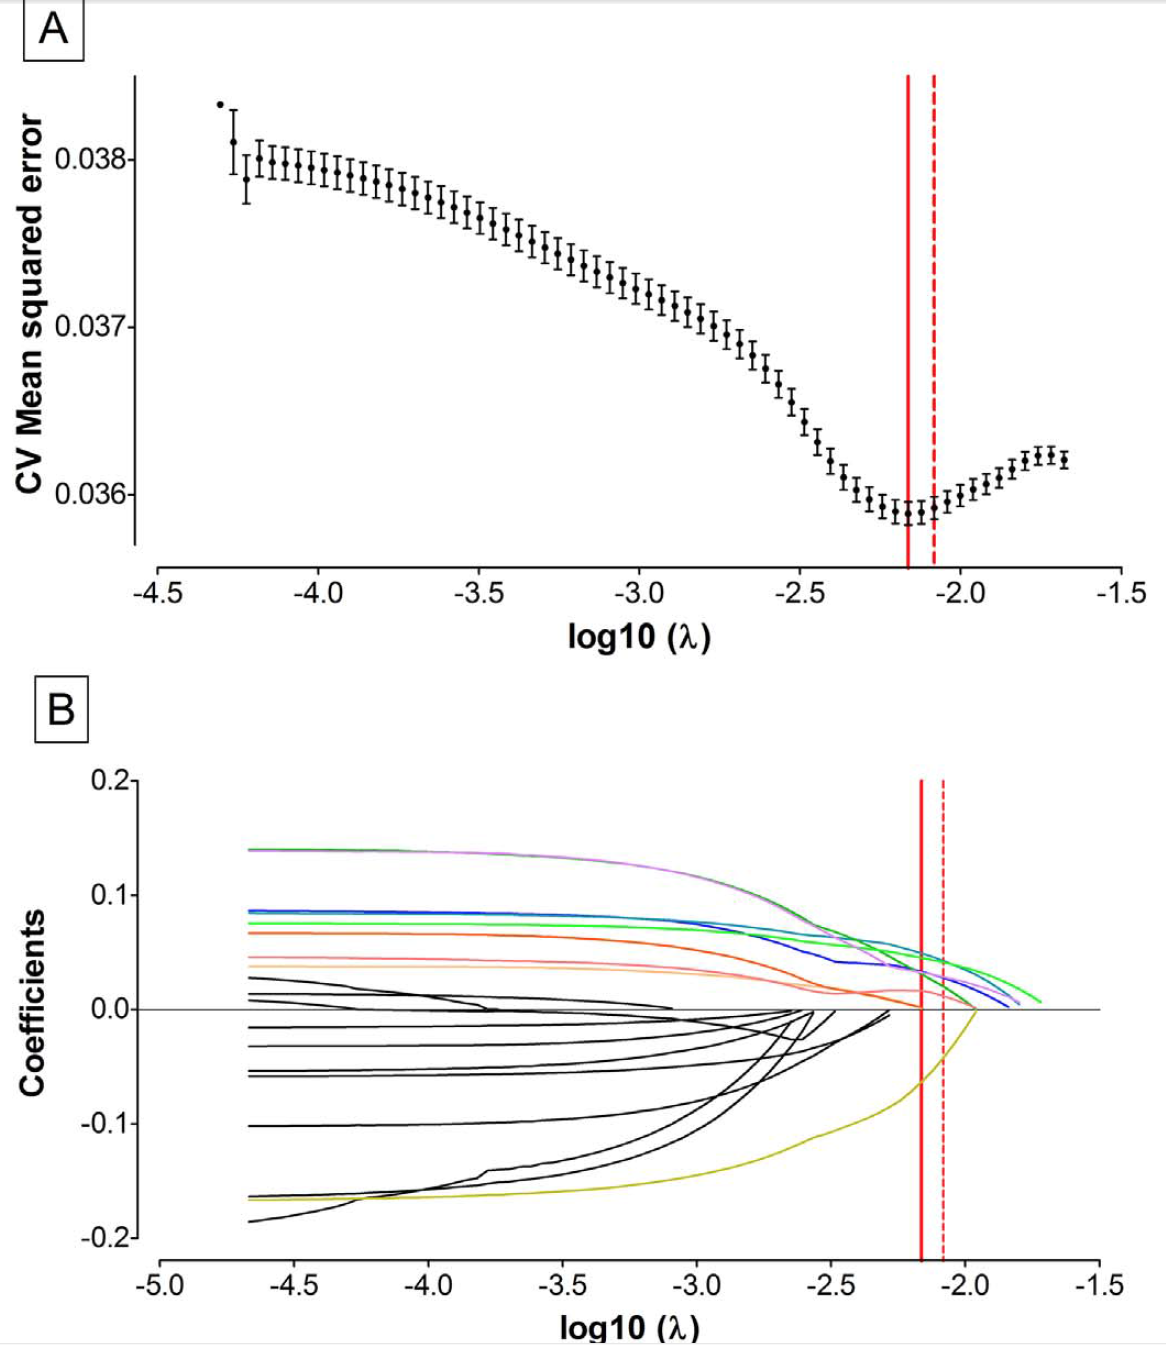
\includegraphics{images/resgraph.png}
\caption{Figure from Vriens et al.}
\end{figure}

\begin{figure}
\centering
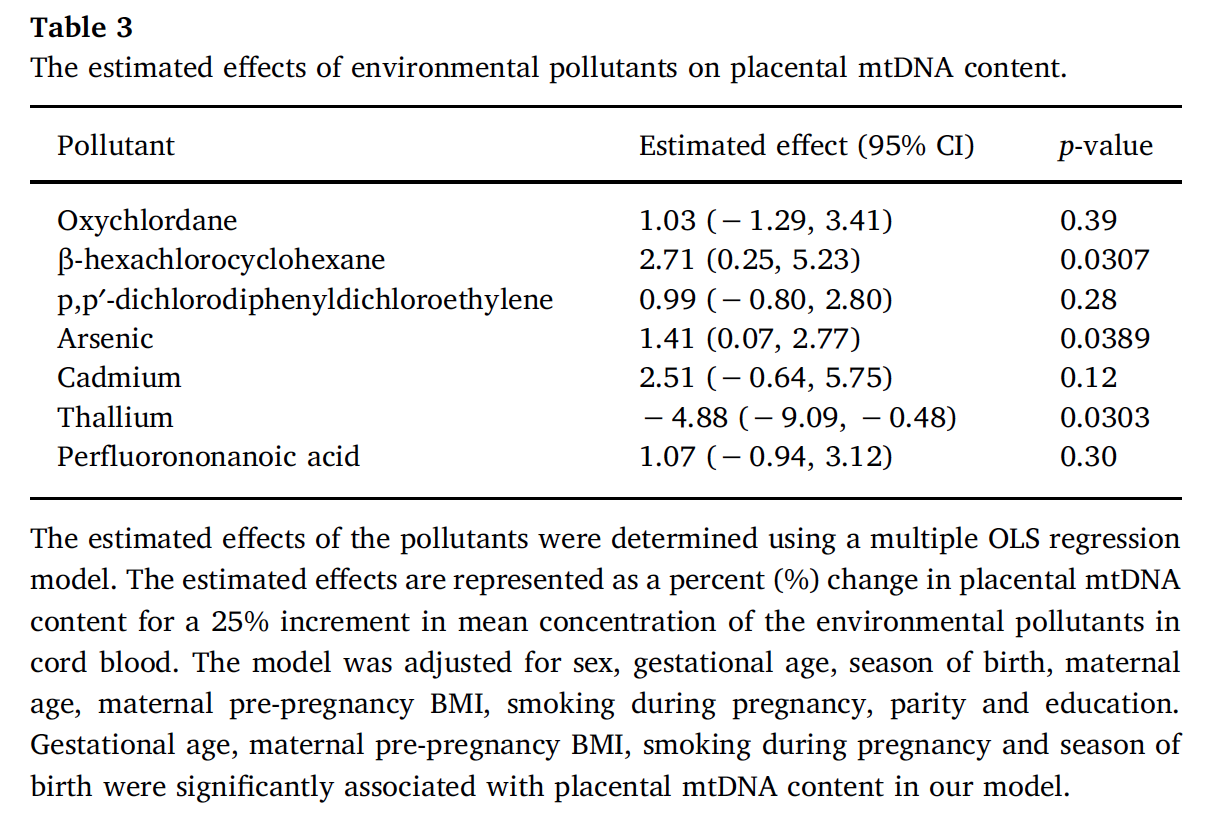
\includegraphics{images/restab.png}
\caption{Table from Vriens et al.}
\end{figure}

\hypertarget{other-regression-based-approaches}{%
\section{Other regression-based approaches}\label{other-regression-based-approaches}}

Before moving on to the a general discussion on advantages and limitations of regression-based approaches, and introduce and motivate further approaches for environmental mixtures, it is useful to provide a broad overview of some alternative approaches based on or derived from classical regression that have proven useful in this context.

\hypertarget{hierarchical-linear-models}{%
\subsection{Hierarchical linear models}\label{hierarchical-linear-models}}

Hierarchical modeling allows improving performances of a multiple regression model when clustering of exposures can be clearly identified. Application of this approach for multiple exposures was first introduced to evaluate the effect of antiretroviral treatments in HIV epidemiology, where several drugs belonging to clearly defined drug classes are usually defined (\citet{correia2019hierarchical}). In brief, the model incorporates first-stage effects for each drug class, and second-stage effects for individual drugs, assuming that the effect of each drug is the summation of the (fixed) effect of its drug class and a residual effect specific to the individual drug. Assuming that we can identify (or observe from preliminary analysis such as a PCA) well characterized subgroups of environmental exposures, this modeling technique can be used to improve the performance of multiple regression when focusing on environmental mixtures. Potential advantages include the absence of variable selection and shrinkage,thus allowing a better interpretation of results.

\hypertarget{partial-least-square-regression}{%
\subsection{Partial least square regression}\label{partial-least-square-regression}}

The Partial least square (PLS) regression can be seen as a method that generalizes and combines PCA and multiple regression. PLS regression is very useful to predict dependent variables from a very large number of predictors that might be highly correlated. The PLS regression replaces the initial independent variable space (X) and the initial response variable space (Y) by smaller spaces that rely on a reduced number of variables named latent variables, which are included one by one in an iterative process. The sparse PLS (sPLS) regression, in particular, is an extension of PLS that aims at combining variable selection and modeling in a one-step procedure (\citet{le2008sparse}). Components are defined iteratively such that they explain as much of the remaining covariance between the predictors and the outcome as possible. The sPLS approach simultaneously yields good predictive performance and appropriate variable selection by creating sparse linear combinations of the original predictors. Sparsity is induced by including a penalty (η) in the estimation of the linear combination coefficients; that is to say, all coefficients with an absolute value lower than some fraction η of the maximum absolute coefficient are shrunk to zero. Only the first K components are included as covariates in a linear regression model, calibrating K and η by minimizing the RMSE using 5-fold cross-validation (the default implementation). sPLS is available in the R package \texttt{spls} , documented \href{https://cran.r-project.org/web/packages/spls/vignettes/spls-example.pdf}{here}. A good illustration of using sPLS in environmental epidemiology can be found in \citet{lenters2015phthalates}.

\hypertarget{advantages-and-limitations-of-regression-approaches}{%
\section{Advantages and limitations of regression approaches}\label{advantages-and-limitations-of-regression-approaches}}

Together with underlying some of the limitations of single and multiple regression in evaluating the effects of environmental mixtures on health outcomes, primarily due to the main problem of multicollinearity, this Section has also introduced techniques that overcome such limitation while remaining embedded in a regression framework. Among these techniques, review articles and simulation studies agree in concluding that penalized regression consistently outperformed conventional approaches, and that the choice of what method to use should be selected based on one-by-one situation. I recommend reading this paper from \citet{agier2016systematic}, systematically comparing methods based on regression in exposome-health analyses.

In practical settings, several research questions can be addressed by using multiple regression or its extensions. Nevertheless, there might be research questions that are beyond the reach of regression techniques and for which some additional methodologies should be considered.

\begin{itemize}
\tightlist
\item
  Assessing the overall mixture effect.
\end{itemize}

Penalized approaches addressed the issues of collinearity and high-dimension by operating some sort of variable selection. While this allows retrieving information on the actual effects for each selected component, addressing other questions such as the ones related to the overall effect of the mixture can not be evaluated. As discussed in Section 1, this is a relevant research question that is often of primary interest. The next section will address this problem, introducing the weighted quantile sum (WQS) regression framework as a technique to evaluate the overall effect of an environmental mixture while taking into account high levels of correlation.

\begin{itemize}
\tightlist
\item
  Complex scenarios with several exposures and interactive mechanisms.
\end{itemize}

When the mixture of interest is composed by several exposures, it is likely that the mixture-outcome association will involve non-linear and interactive mechanisms. As the number of potential predicors gets higher, so does the complexity of the model. In such situations the performances of regression-based approaches are generally weak, and more flexible algorithms should be taken into considerations. These problems will be assessed in section 6, introducing Bayesian kernel Machine Regression as a flexible non-parametric approach to estimate the mixture-outcome association in the presence of complex non-linear and interactive mechanisms, and then discussing techniques for the assessment of high-dimensional interactions, including machine learning algorithms based on trees modeling.

\hypertarget{assessing-the-overall-cumulative-effect-of-multiple-exposures}{%
\chapter{Assessing the overall (cumulative) effect of multiple exposures}\label{assessing-the-overall-cumulative-effect-of-multiple-exposures}}

Extensions of linear regression presented in the previous chapter address the complexity of the mixture-outcome association by selecting relevant predictors within the mixture, thus removing covariates that would create problems due to high collinearity, or simply by reducing the dimension of the exposure matrix thus improving the fit of the model. This approach, however, also comes with relevant drawbacks.

Let's think of the group of highly correlated exposures from our hypothetical example (\(X_3-X_4-X_5\)), where penalized approaches recommended only selecting \(X_4\). This allowed evaluating the independent effect of \(X_4\) on the outcome without being troubled by the high levels of correlation between this covariate and the other 2 of the cluster. This same selection, however, is preventing us to address other important questions. For example, what if there is an interaction between \(X_3\) and \(X_4\) (this can happen even if \(X_3\) does not have an independent effect on the outcome, but only an effect that is triggered in the presence of the other co-exposure)? By removing \(X_3\) from the model, we will not be able to evaluate this interaction. Moreover, we will not be able to correctly quantify the joint effect of \(X_3\) and \(X_4\), which is the sum of the two main effects and their 2-way interaction. As discussed in the first chapter, this is a very important research question: the three correlated exposures might for instance come from the same source, and quantifying their joint effect would in this case provide useful information on the public health benefits of reducing exposure to the source.

The question that we will address in this section is the following: how do we quantify the joint effect of several exposures, possibly highly correlated, when regression techniques are not functional?

\hypertarget{unsupervised-summary-scores}{%
\section{Unsupervised summary scores}\label{unsupervised-summary-scores}}

A very intuitive approach is to create one or more summary score(s) that summarize individual levels of exposure to the mixture, thus reducing the numbers of covariates that are going to be evaluated. A very common example of such approach is used by investigators working on phthalates. In this context, analyses are often hampered by the presence of extreme correlation between metabolites of Di(2-ethylhexyl)phthalate (DEHP), and researchers are commonly summarizing this information into a molar sum of DEHP. \citet{li2019serum} writes, for example ``we calculated the molar sum of DEHP metabolites (ΣDEHP) by dividing
each metabolite concentration by its molecular weight and then
summing: ΣDEHP={[}MEHP (μg/L)×(1/278.34 (g/mol)){]}+{[}MEHHP
(μg/L) × (1/294.34 (g/mol)){]} + {[}MEOHP (μg/L) × (1/292.33 (g/
mol)){]} + {[}MECPP (μg/L) × (1/308.33 (g/mol)){]}''. Note that, with this approach, the score targets a selected sub-sample of exposures (the highly-correlated cluster creating problems), and other phthalates metabolites are included in the model without any transformation.

Another common approach is to use components derived from PCA, as described in section 3. PCA allows identifying continuous covariates that summarize the variability of the mixture exposure. Including these derived components into a regression model has the great advantage that all collinearity issues will be resolved, as the components are uncorrelated by definition. On the other hand, the validity of this approach is severely affected by whether the obtained components have clear biological interpretation. A good example of this approach can be found in \citet{souter2020urinary}.

\hypertarget{weighted-quantile-sum}{%
\section{Weighted quantile sum}\label{weighted-quantile-sum}}

Taking one step further, researchers might be interested in taking into account the relationship between the exposures and the outcome while summarizing the complex exposure to the mixture of interest. The weighted quantile sum (WQS), developed specifically for the context of environmental mixtures analysis, is an increasingly common approach that allows evaluating a mixture-outcome association by creating a summary score of the mixture in a supervised fashion (\citet{czarnota2015assessment}), (\citet{carrico2015characterization}). Specifically, WQS is a statistical model for multivariate regression in high-dimensional dataset that operates in a supervised framework, creating a single score (the weighted quantile sum) that summarizes the overall exposure to the mixture, and by including this score in a regression model to evaluate the overall effect of the mixture on the outcome of interest. The score is calculated as a weighted sum (so that exposures with weaker effects on the outcome have lower weight in the index) of all exposures categorized into quartiles, or more groups (so that extreme values have less impact on the weight estimation.

\hypertarget{model-definition-and-estimation}{%
\subsection{Model definition and estimation}\label{model-definition-and-estimation}}

Most of what follows in this subsection is taken from the excellent introductory material shared online by Dr.~Renzetti at this \href{https://cran.r-project.org/web/packages/gWQS/vignettes/gwqs-vignette.html}{link}, which should be referred to for further details on the technique.

The WQS model takes the following form:

\begin{equation} \label{eq:wqs}
g(\mu) = \beta_0 + \beta_1\Bigg(\sum_{i=1}^{c}w_iq_i\Bigg) + \boldsymbol{z'\varphi}
\end{equation}

The \((\sum_{i=1}^{c}w_iq_i)\) term represents the index that weights and sums the components included in the mixture. As such, \(\beta_1\) will be the parameter summarizing the overall effect to the (weighted) mixture. In addition, the model will also provide an estimate of the individual weights \(w_i\) that indicate the relative importance of each exposure in the mixture-outcome association.

To estimate the model, the data may be split in a training and a validation dataset: the first one to be used for the weight estimation, the second one to test for the significance of the final WQS index. The weights are estimated through a bootstrap and constrained to sum to one and bounded between zero and one: \(\sum_{i=1}^{c}w_i=1\) and \(0 \leq w_i \leq 1\). For each bootstrap sample (usually \(B=100\) total samples) a dataset is created sampling with replacement from the training dataset and the parameters of the model are estimated through an optimization algorithm.An inequality constraint is also applied in order to impose that \(0 \leq w_i \leq 1\).

Once the weights are estimated, the model is fitted in order to find the regression coefficients in each ensemble step. After the bootstrap ensemble is completed, the estimated weights are averaged across bootstrap samples to obtain the WQS index:

\[WQS = \sum_{i=1}^c \bar{w}_iq_i\]

Typically weights are estimated in a training set then used to construct a WQS index in a validation set, which can be used to test for the association between the mixture and the health outcome in a standard generalized linear model, as:

\[g(\mu) = \beta_0 + \beta_1WQS + \boldsymbol{z'\varphi}\]

After the final model is fitted one can test the significance of the \(\beta_1\) to see if there is an association between the WQS index and the outcome. In the case the coefficient is significantly different from 0 then we can interpret the weights: the highest values identify the associated components as the relevant contributors in the association. A selection threshold can be decided a priori as \(\tau = 1/c\) to identify those chemicals that have a significant weight in the index.

\hypertarget{the-unidirectionality-assumption}{%
\subsection{The unidirectionality assumption}\label{the-unidirectionality-assumption}}

WQS makes an important assumption of uni-direction (either a positive or a negative) of all exposures with respect to the outcome. The model is inherently one-directional, in that it tests only for mixture effects positively or negatively associated with a given outcome. In practice analyses should therefore be run twice to test for associations in either direction.

The one-directional index allows not to incur in the reversal paradox when we have highly correlated variables thus improving the identification of bad actors.

\hypertarget{extensions-of-the-original-wqs-regression}{%
\subsection{Extensions of the original WQS regression}\label{extensions-of-the-original-wqs-regression}}

\begin{itemize}
\tightlist
\item
  Dependent variables
\end{itemize}

The WQS regression can be generalized and applied to multiple types of dependent variables. In particular, WQS regression has been adapted to four different cases: logistic, multinomial, Poisson and negative binomial regression. For these last two cases it is also possible to fit zero-inflated models keeping the same objective function used to estimate the weights as for the Poisson and negative binomial regression but taking into account the zero inflation fitting the final model.

\begin{itemize}
\tightlist
\item
  Random selection
\end{itemize}

A novel implementation of WQS regression for high-dimensional mixtures with highly correlated components was proposed in \citet{curtin2021random}. This approach applies a random selection of a subset of the variables included in the mixture instead of the bootstrapping for parameter estimation. Through this method we are able to generate a more de-correlated subsets of variables and reduce the variance of the parameter estimates compared to a single analysis. This novel statistical methodology was shown to be more effective compared to WQS in modeling contexts with large predictor sets, complex correlation structures, or where the numbers of predictors exceeds the number of subjects.

\begin{itemize}
\tightlist
\item
  Repeated holdout validation for WQS regression
\end{itemize}

One limit of WQS is the reduced statistical power caused by the necessity to split the dataset in training and validation sets. This partition can also lead to unrepresentative sets of data and unstable parameter estimates. A recent work from \citet{tanner2019repeated} showed that conducing a WQS on the full dataset without splitting in training and validation produces optimistic results and proposed to apply a repeated holdout validation combining cross-validation and bootstrap resampling. They suggested to repeatedly split the data 100 times with replacement and fit a WQS regression on each partitioned dataset. Through this procedure we obtain an approximately normal distribution of the weights and the regression parameters and we can apply the mean or the median to estimate the final parameters. A limit of this approach is the higher computational intensity.

\begin{itemize}
\tightlist
\item
  Additional approaches
\end{itemize}

To complete the set of currently available extensions of this approach, it is finally worthy to mention the Bayesian WQS (\citet{colicino2020per}), which also allows relaxing the uni-directional assumption, and the lagged WQS (\citet{gennings2020lagged}), which deals with time-varying mixtures of exposures to understand the role of exposure timing.

\hypertarget{quantile-g-computation}{%
\subsection{Quantile G-computation}\label{quantile-g-computation}}

A recent paper by \citet{keil2020quantile} introduced an additional modeling technique for environmental mixture that builds up on WQS regression integrating its estimation procedure with g-computation. This approach, called Quantile-based g-Computation estimates the overall mixture effect with the same procedure used by WQS, but estimating the parameters of a marginal structural model, rather than a standard regression. In this way, under common assumptions in causal inference such as exchangeability, causal consistency, positivity, no interference, and correct model specification, this model will also improve the causal interpretation of the overall effect. Importantly, the procedure also allegedly overcomes the assumption of uni-direction, and the flexibility of marginal structural models also allows incorporating non-linearities in the contribution of each exposure to the score. Additional details on the models can be found on the original paper or in this useful R \href{https://cran.r-project.org/web/packages/qgcomp/vignettes/qgcomp-vignette.html}{vignette}.

\hypertarget{wqs-regression-in-r}{%
\subsection{WQS regression in R}\label{wqs-regression-in-r}}

WQS is available in the R package \texttt{gWQS} (standing for generalized WQS). Documentation and guidelines can be found \href{https://cran.r-project.org/web/packages/gWQS/gWQS.pdf}{here}. Note that if you are working on a mac with a OS different than OS 10.5 through 10.7, you may have to install X Quartz at \url{https://www.xquartz.org}, before being able to load the \texttt{gWQS} library. The recently developed quantile G-computation approach is instead available in the \texttt{qgcomp} package.

Fitting WQS in R will require some additional data management. First of all, both \texttt{gWQS} and \texttt{qgcomp} will require an object with the \textbf{names} of the exposures, rather than a matrix with the exposures themselves.

\begin{Shaded}
\begin{Highlighting}[]
\NormalTok{exposure}\OtherTok{\textless{}{-}} \FunctionTok{names}\NormalTok{(data2[,}\DecValTok{3}\SpecialCharTok{:}\DecValTok{16}\NormalTok{])}
\end{Highlighting}
\end{Shaded}

The following lines will fit a WQS regression model for the positive direction, with a 40-60 training validation split, and without adjusting for covariates. The reader can refer to the link above for details on all available options.

\begin{Shaded}
\begin{Highlighting}[]
\NormalTok{results1 }\OtherTok{\textless{}{-}} \FunctionTok{gwqs}\NormalTok{(y }\SpecialCharTok{\textasciitilde{}}\NormalTok{ wqs, }\AttributeTok{mix\_name =}\NormalTok{ exposure, }\AttributeTok{data =}\NormalTok{ data2, }\AttributeTok{q =} \DecValTok{4}\NormalTok{, }\AttributeTok{validation =} \FloatTok{0.6}\NormalTok{,}
                \AttributeTok{b =} \DecValTok{10}\NormalTok{, }\AttributeTok{b1\_pos =}\NormalTok{ T, }\AttributeTok{b1\_constr =}\NormalTok{ F, }\AttributeTok{family =} \StringTok{"gaussian"}\NormalTok{, }
                \AttributeTok{seed =} \DecValTok{123}\NormalTok{)}
\end{Highlighting}
\end{Shaded}

After fitting the model, this set of lines will produce a barplot with the weights as well as the summary of results (overall effect and weights estimation)

\begin{Shaded}
\begin{Highlighting}[]
\FunctionTok{gwqs\_barplot}\NormalTok{(results1, }\AttributeTok{tau=}\ConstantTok{NULL}\NormalTok{)}
\end{Highlighting}
\end{Shaded}

\begin{figure}[H]

{\centering 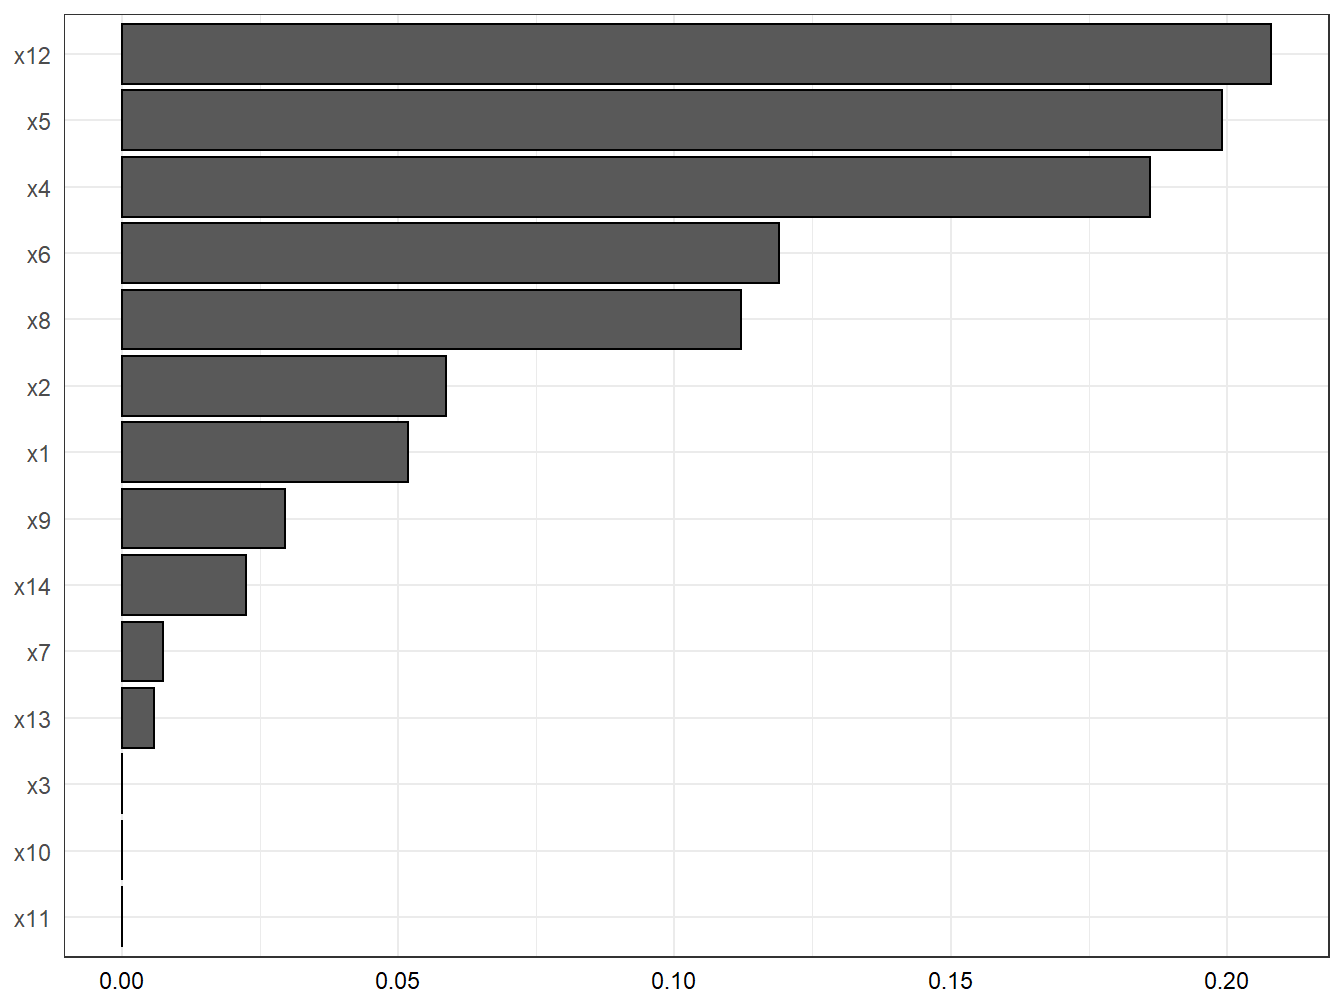
\includegraphics[width=0.8\linewidth]{bookdown-demo_files/figure-latex/figureenetadjx-1} 

}

\caption{WQS: weights estimation}\label{fig:figureenetadjx}
\end{figure}

Here the actual estimates that are being plotted:

\begin{table}

\caption{\label{tab:unnamed-chunk-22}WQS: weights estimation}
\centering
\begin{tabular}[t]{l|l|r}
\hline
  & mix\_name & mean\_weight\\
\hline
x12 & x12 & 0.2080444\\
\hline
x5 & x5 & 0.1990505\\
\hline
x4 & x4 & 0.1860921\\
\hline
x6 & x6 & 0.1190146\\
\hline
x8 & x8 & 0.1120772\\
\hline
x2 & x2 & 0.0586329\\
\hline
x1 & x1 & 0.0518465\\
\hline
x9 & x9 & 0.0295788\\
\hline
x14 & x14 & 0.0224343\\
\hline
x7 & x7 & 0.0074698\\
\hline
x13 & x13 & 0.0057590\\
\hline
x3 & x3 & 0.0000000\\
\hline
x10 & x10 & 0.0000000\\
\hline
x11 & x11 & 0.0000000\\
\hline
\end{tabular}
\end{table}

To estimate the negative index, still without direct constraint on the actual \(\beta\), we change the \texttt{b1\_pos} option to FALSE. In this situation, all bootstrap samples provide a positive coefficient. This suggests that we are in a situation where all covariates have a positive (or null) effect. Even constraining the coefficient would likely not make any difference in this case - coefficients would either be all around 0, or the model will not converge. For the next points, therefore, we will only focus on the positive index.

To adjust for covariates we can add them in the model as presented here:

\begin{Shaded}
\begin{Highlighting}[]
\NormalTok{results1\_0\_adj }\OtherTok{\textless{}{-}} \FunctionTok{gwqs}\NormalTok{(y }\SpecialCharTok{\textasciitilde{}}\NormalTok{ wqs}\SpecialCharTok{+}\NormalTok{z1}\SpecialCharTok{+}\NormalTok{z2}\SpecialCharTok{+}\NormalTok{z3, }\AttributeTok{mix\_name =}\NormalTok{ exposure, }\AttributeTok{data =}\NormalTok{ data2, }\AttributeTok{q =} \DecValTok{4}\NormalTok{, }\AttributeTok{validation =} \FloatTok{0.6}\NormalTok{,}
                \AttributeTok{b =} \DecValTok{10}\NormalTok{, }\AttributeTok{b1\_pos =}\NormalTok{ T, }\AttributeTok{b1\_constr =}\NormalTok{ F, }\AttributeTok{family =} \StringTok{"gaussian"}\NormalTok{, }
                \AttributeTok{seed =} \DecValTok{123}\NormalTok{)}
\end{Highlighting}
\end{Shaded}

\begin{Shaded}
\begin{Highlighting}[]
\FunctionTok{gwqs\_barplot}\NormalTok{(results1\_0\_adj, }\AttributeTok{tau=}\ConstantTok{NULL}\NormalTok{)}
\end{Highlighting}
\end{Shaded}

\begin{figure}[H]

{\centering 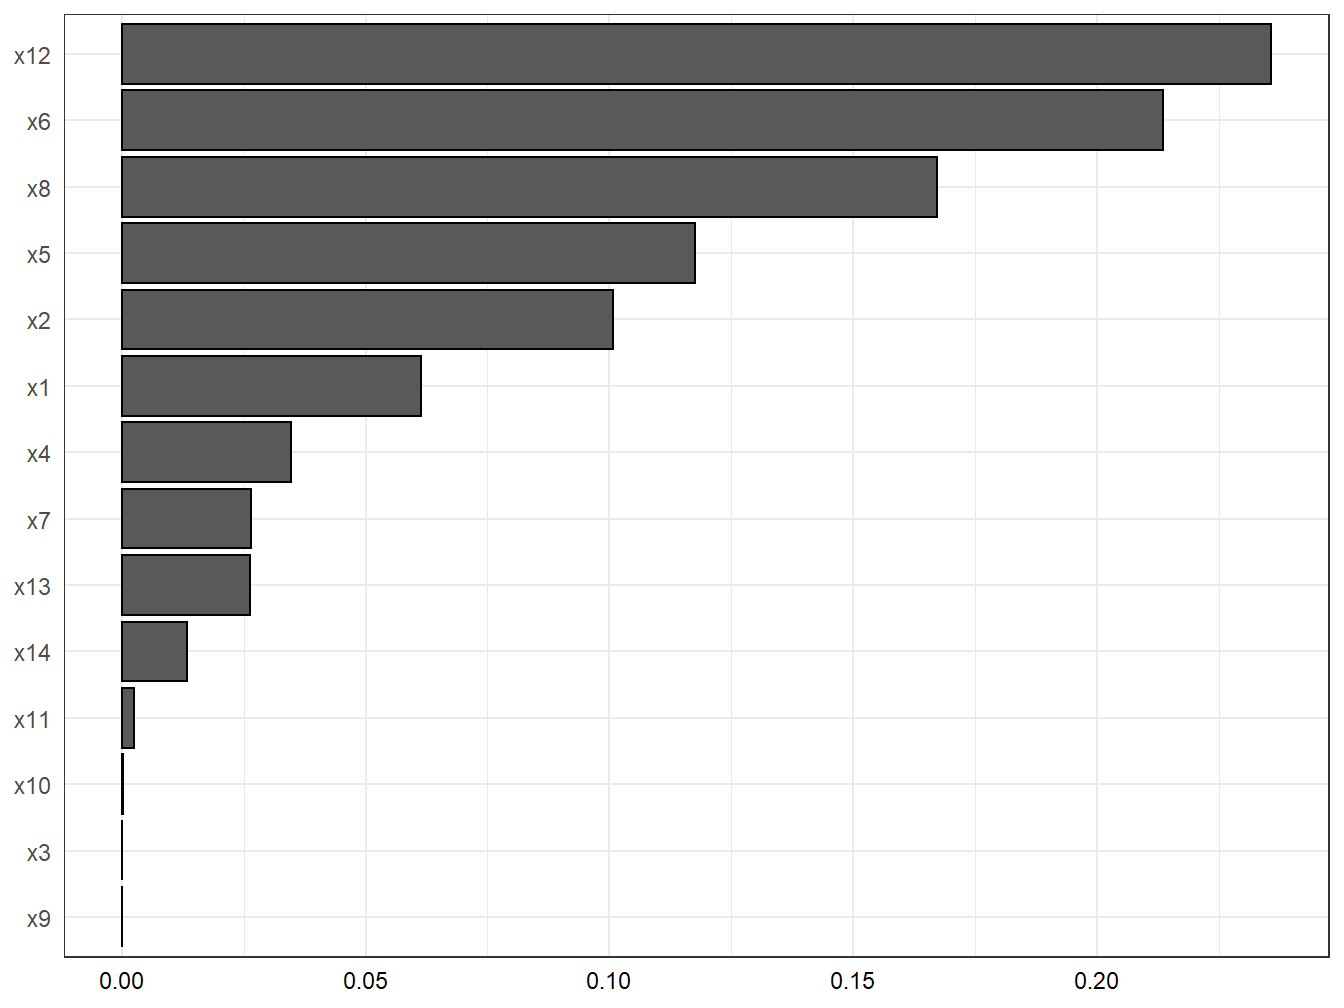
\includegraphics[width=0.8\linewidth]{bookdown-demo_files/figure-latex/figureenetadj-1} 

}

\caption{WQS: weights estimation with covariates adjustment}\label{fig:figureenetadj}
\end{figure}

After adjustment the association is largely attenuated, and the weights of the most important contributors change both in magnitude as well as in ranking. This implies that the three confounders have a different effect on each of the components (e.g.~the contribution of \(X_6\) was attenuated before adjusting, while the contribution of \(X_4\) was overestimated).

The following lines will fit a quantile G-computation model. What we have to specify in the command is the list of exposures, the name of the mixture object, the data, the type of outcome (continuous here), and whether we want quartiles or other categorizations.

\begin{Shaded}
\begin{Highlighting}[]
\NormalTok{qc }\OtherTok{\textless{}{-}} \FunctionTok{qgcomp}\NormalTok{(y }\SpecialCharTok{\textasciitilde{}}\NormalTok{ x1}\SpecialCharTok{+}\NormalTok{x2}\SpecialCharTok{+}\NormalTok{x3}\SpecialCharTok{+}\NormalTok{x4}\SpecialCharTok{+}\NormalTok{x5}\SpecialCharTok{+}\NormalTok{x6}\SpecialCharTok{+}\NormalTok{x7}\SpecialCharTok{+}\NormalTok{x8}\SpecialCharTok{+}\NormalTok{x9}\SpecialCharTok{+}\NormalTok{x10}\SpecialCharTok{+}\NormalTok{x11}\SpecialCharTok{+}\NormalTok{x12}\SpecialCharTok{+}\NormalTok{x13}\SpecialCharTok{+}\NormalTok{x14}
                         \SpecialCharTok{+}\NormalTok{z1}\SpecialCharTok{+}\NormalTok{z2}\SpecialCharTok{+}\NormalTok{z3,}
                         \AttributeTok{expnms=}\NormalTok{exposure,}
\NormalTok{                         data2, }\AttributeTok{family=}\FunctionTok{gaussian}\NormalTok{(), }\AttributeTok{q=}\DecValTok{4}\NormalTok{)}
\end{Highlighting}
\end{Shaded}

\begin{Shaded}
\begin{Highlighting}[]
\FunctionTok{plot}\NormalTok{(qc)}
\end{Highlighting}
\end{Shaded}

\begin{figure}[H]

{\centering 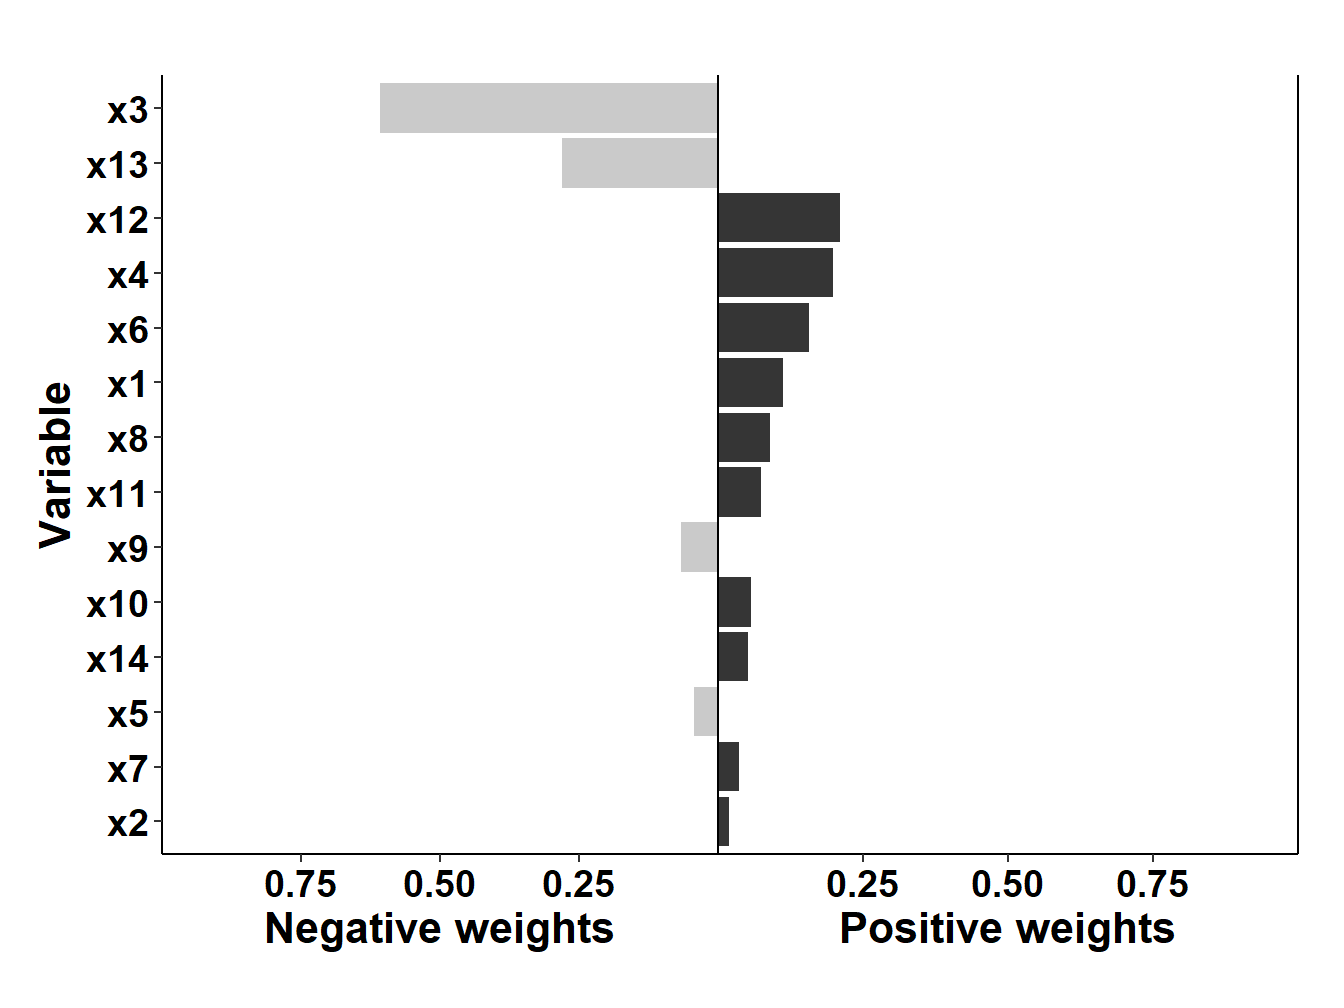
\includegraphics[width=0.8\linewidth]{bookdown-demo_files/figure-latex/figureenetadja-1} 

}

\caption{qgcomp: weights estimation with covariates adjustment}\label{fig:figureenetadja}
\end{figure}

The Authors also recommended fitting the model using bootstrap, which can be achieved with the following command. Note that the number of iterations, her set to 10, should be at least 200. The plot from this model will provide the estimate of the overall effect of the mixture.

\begin{Shaded}
\begin{Highlighting}[]
\NormalTok{qc.boot }\OtherTok{\textless{}{-}} \FunctionTok{qgcomp.boot}\NormalTok{(y }\SpecialCharTok{\textasciitilde{}}\NormalTok{ x1}\SpecialCharTok{+}\NormalTok{x2}\SpecialCharTok{+}\NormalTok{x3}\SpecialCharTok{+}\NormalTok{x4}\SpecialCharTok{+}\NormalTok{x5}\SpecialCharTok{+}\NormalTok{x6}\SpecialCharTok{+}\NormalTok{x7}\SpecialCharTok{+}\NormalTok{x8}\SpecialCharTok{+}\NormalTok{x9}\SpecialCharTok{+}\NormalTok{x10}\SpecialCharTok{+}\NormalTok{x11}\SpecialCharTok{+}\NormalTok{x12}\SpecialCharTok{+}\NormalTok{x13}\SpecialCharTok{+}\NormalTok{x14}
                         \SpecialCharTok{+}\NormalTok{z1}\SpecialCharTok{+}\NormalTok{z2}\SpecialCharTok{+}\NormalTok{z3,}
                         \AttributeTok{expnms=}\NormalTok{exposure,}
\NormalTok{                         data2, }\AttributeTok{family=}\FunctionTok{gaussian}\NormalTok{(), }\AttributeTok{q=}\DecValTok{4}\NormalTok{, }\AttributeTok{B=}\DecValTok{10}\NormalTok{, }\AttributeTok{seed=}\DecValTok{123}\NormalTok{)}
\end{Highlighting}
\end{Shaded}

\begin{Shaded}
\begin{Highlighting}[]
\FunctionTok{plot}\NormalTok{(qc.boot)}
\end{Highlighting}
\end{Shaded}

\begin{figure}[H]

{\centering 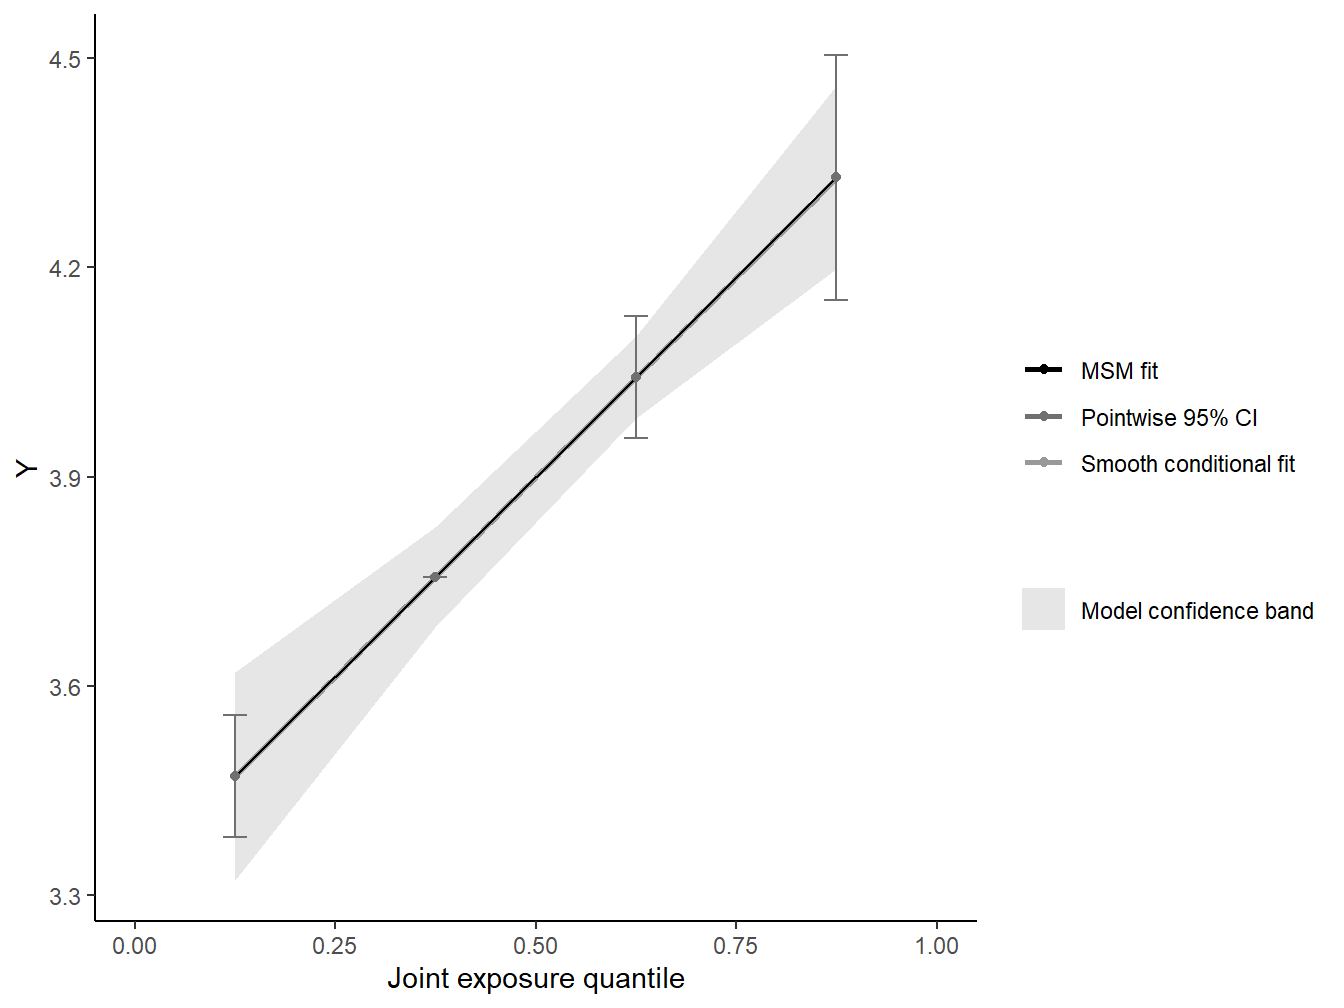
\includegraphics[width=0.8\linewidth]{bookdown-demo_files/figure-latex/figureenetadjsZCV-1} 

}

\caption{qgcomp: overall effect}\label{fig:figureenetadjsZCV}
\end{figure}

It is interesting to note that in this situation of high-collinearity, qgcomp's results are still affected as we see a strikingly high (and, as we know since data are simulated, wrong) negative weight for \(X_3\).

A final note: both packages are very recent and constantly updated and revised. You should always refer to the vignette and documentation provided above for updates and eventual modification in the syntax.

\hypertarget{example-from-the-literature}{%
\subsection{Example from the literature}\label{example-from-the-literature}}

Thanks for its easy implementation in statistical software and the development of the several discussed extensions, WQS is rapidly becoming one of the most common techniques used by investigators to evaluate environmental mixtures.

As an illustrative example on how methods and results can be presented the reade can refer to , we can use the paper from \citet{deyssenroth2018intrauterine}, evaluating the association between 16 trace metals, measured in post-partum maternal toe nails in about 200 pregnant women from the Rhode Island Child Health Study, and small for gestational age (SGA) status. before fitting WQS the Authors conduct a preliminary analysis using conditional logistic regression, which indicates that effects seem to operate in both directions.

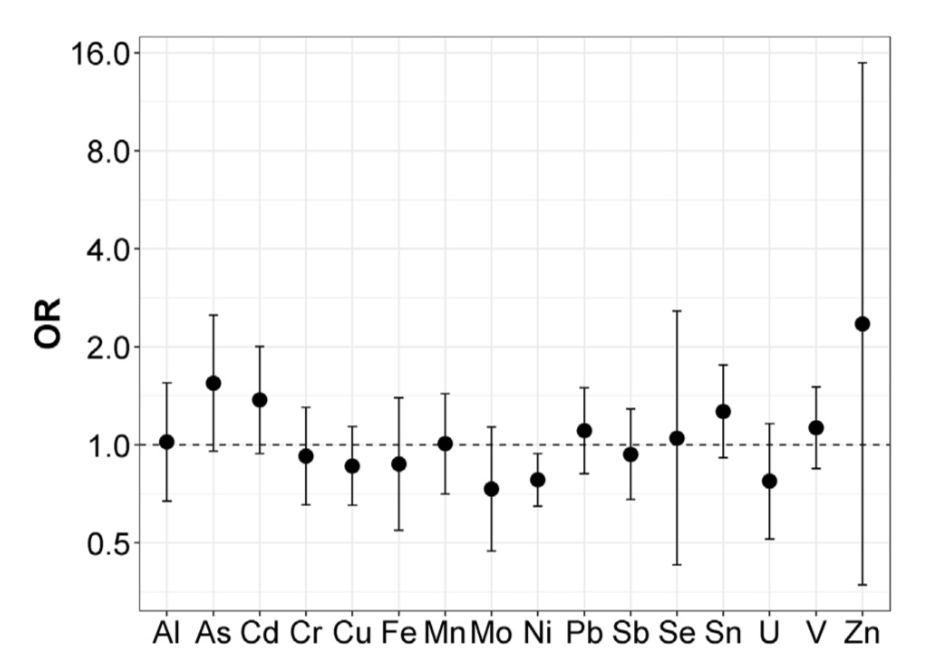
\includegraphics{images/deyslog.png}
As a consequence, WQS results are presented for both the positive and negative directions, summarizing both weights estimates and total effects in a clear and informative figure.

\begin{figure}
\centering
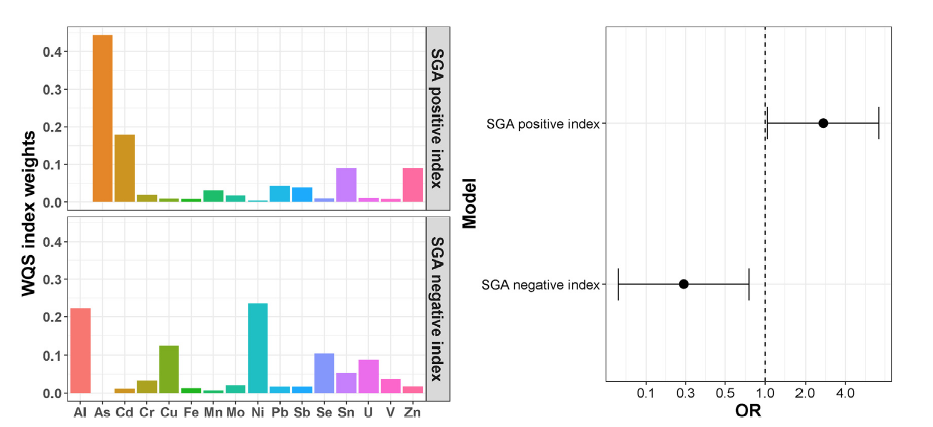
\includegraphics{images/deys.png}
\caption{WQS results from Deyssenroth et al.}
\end{figure}

\hypertarget{flexible-approaches-for-complex-settings}{%
\chapter{Flexible approaches for complex settings}\label{flexible-approaches-for-complex-settings}}

In the previous sections we have discussed the challenges that arise when evaluating environmental mixtures and the several available techniques based on regression modeling that can be used to to address different research questions in this context. The final section of section 4 discussed the 2 major limitations shared by all regression techniques, namely the difficulties in estimating overall mixture effects and to include additional model complexities such as non-linearities and (possibly high-order) interactions. In the previous section we have discussed WQS as a useful tool to address the first limitation. Note than, interestingly, this technique can be actually seen as yet another regression extension, as it is based on integrating a summary score into a generalized linear model.

To tackle the second challenge, let's first note that any regression would allow integrating interactions of any order (this is done by simply including product terms between any pair, or higher combination, of exposures) as well as non-linear associations. Splines modeling is probably the best way of accounting for non-linear effects in regression modeling, and one can also consider using generalized additive models (GAM), which have been successfully applied in the context of environmental mixtures (\citet{zheng2020evaluating}). Nevertheless, both the inclusion of product terms and spline transformations will rapidly increase the number of parameters that are to be estimated, and we might be in need of alternative techniques that can more flexibly tackle these issues. In this context, we are going to describe two approaches: first, bayesian kernel machine regression (BKMR), a method directly developed for evaluating environmental mixtures that is increasing in popularity because of its several advantages and flexibility (\citet{bobb2015bayesian}),(\citet{bobb2018statistical}). Second, the use of machine learning techniques, and specifically tree-based modeling such as boosted regression trees (\citet{lampa2014identification}),(\citet{bellavia2021joint}). Additional techniques that can be considered when the specific focus is on detecting interactions will not be discussed here, and the reader can refer to these publications summarizing and discussing methodologies in this context: \citet{barrera2017systematic}, \citet{sun2013statistical}.

\hypertarget{bayesian-kernel-machine-regression}{%
\section{Bayesian Kernel Machine Regression}\label{bayesian-kernel-machine-regression}}

The material presented in this section is largely taken from Prof.~Coull's guest lectures material and Dr.~Bobb's \href{https://jenfb.github.io/bkmr/overview.html}{vignette}.

\hypertarget{introduction-1}{%
\subsection{Introduction}\label{introduction-1}}

Possible objectives of a mixtures analysis could include detection and estimation of an effect of the overall mixture,
identification of pollutant or group of pollutants responsible for
observed mixture effects,visualizing the exposure-response function, or
detection of interactions among individual pollutants. Bayesian Kernel Machine Regression (BKMR) is designed to address all
four of these objectives in a flexible non-parametric way. The main idea of BKMR is to model exposure through means of a kernel function. Specifically, the general modeling framework is

\[Y_i=h(z_{i1},…,z_{iM})+βx_i+\epsilon_i\]

where \(Y_i\) is a continuous, normally distributed health endpoint, \(h\) is a flexible function of the predictor variables \(z_{i1},…,z_{iM}\), and \(x_i\) is a vector of covariates assumed to have a linear relationship with the outcome

There are several choices for the kernel function used to represent \(h\). The focus here is on the Gaussian kernel, which flexibly captures a wide range of underlying functional forms for h and can accommodate nonlinear and non-additive effects of the
multivariate exposure. Specifically, the Gaussian kernel implies the following representation for \(h\):

\[K_{vs}(z_i,z_j)=exp\{-\sum_{M}r_m(z_{im}-z_{jm})^2\}\]

Intuitively, the kernel function shrinks the estimated health effects of two individuals with similar exposure profiles toward each other. The weights \(r_m\) present the probability that each exposure is important in the function, with \(r_m=0\) indicating that there is no association between the \(m^{th}\) exposure and the outcome. By allowing some weights to be 0, the method is implicitly embedding a variable selection procedure. This can also integrate information on existing structures among exposures (e.g.~correlation clusters, PCA results, similar mechanisms \ldots) with the so-called hierarchical variable selection, which estimates the probability each group of exposures is important, and the probability that, given a group is important, each
exposure in that group is driving that group-outcome association.

\hypertarget{estimation}{%
\subsection{Estimation}\label{estimation}}

BKMR takes its full name from the Bayesian approach used for estimating the parameters. The advantages of this include the ability of estimating the importance of each variable (\(r_m\)) simultaneously, estimating uncertainties measures, and easily extending the estimation to longitudinal data. Since the estimation is built within an iterative procedure (MCMC), variable importance are provided in terms of Posterior Inclusion Probability (PIP), the proportion of iterations with \(r_m>0\). Typically, several thousands of iterations are required.

The \texttt{bkmr} R package developed by the Authors makes implementation of this technique relatively straightforward.

Using our illustrative example, the following chunk of code includes a set of lines required before estimating a BKMR model. Specifically, we are defining the object containing the mixture (\(X_{1}-X_{14}\)), the outcome (\(Y\)), and the confounders (\(Z_1-Z_3\)). We also need to generate a seed (we are using an iterative process with a random component) and a knots matrix that will help speeding up the process. This final step is very important as the model estimation can be extremely long (the recommendation is to use a number of knots of more or less n/10).

\begin{Shaded}
\begin{Highlighting}[]
\NormalTok{mixture}\OtherTok{\textless{}{-}}\FunctionTok{as.matrix}\NormalTok{(data2[,}\DecValTok{3}\SpecialCharTok{:}\DecValTok{16}\NormalTok{])}
\NormalTok{y}\OtherTok{\textless{}{-}}\NormalTok{data2}\SpecialCharTok{$}\NormalTok{y}
\NormalTok{covariates}\OtherTok{\textless{}{-}}\FunctionTok{as.matrix}\NormalTok{(data2[,}\DecValTok{17}\SpecialCharTok{:}\DecValTok{19}\NormalTok{])}

\FunctionTok{set.seed}\NormalTok{(}\DecValTok{10}\NormalTok{)}
\NormalTok{knots100  }\OtherTok{\textless{}{-}}\NormalTok{ fields}\SpecialCharTok{::}\FunctionTok{cover.design}\NormalTok{(mixture, }\AttributeTok{nd =} \DecValTok{50}\NormalTok{)}\SpecialCharTok{$}\NormalTok{design}
\end{Highlighting}
\end{Shaded}

The actual estimation of a BKMR model is very simple and requires one line of R code. With the following lines we fit a BKMR model with Gaussian predictive process using 100 knots. We are using 1000 MCMC iterations for the sake of time, but your final analysis should be run on a much larger number of samples, up to 50000. Here we are allowing for variable selection, but not providing any information on grouping.

\begin{Shaded}
\begin{Highlighting}[]
\NormalTok{temp }\OtherTok{\textless{}{-}}  \FunctionTok{kmbayes}\NormalTok{(}\AttributeTok{y=}\NormalTok{y, }\AttributeTok{Z=}\NormalTok{mixture, }\AttributeTok{X=}\NormalTok{covariates, }\AttributeTok{iter=}\DecValTok{1000}\NormalTok{, }\AttributeTok{verbose=}\ConstantTok{FALSE}\NormalTok{, }\AttributeTok{varsel=}\ConstantTok{TRUE}\NormalTok{, }
                 \AttributeTok{knots=}\NormalTok{knots100)}

\FunctionTok{ExtractPIPs}\NormalTok{(temp)}
\end{Highlighting}
\end{Shaded}

\begin{verbatim}
##    variable   PIP
## 1        x1 0.110
## 2        x2 0.082
## 3        x3 0.000
## 4        x4 0.000
## 5        x5 0.072
## 6        x6 0.142
## 7        x7 0.000
## 8        x8 0.336
## 9        x9 0.062
## 10      x10 0.400
## 11      x11 0.188
## 12      x12 0.818
## 13      x13 0.080
## 14      x14 0.158
\end{verbatim}

The \texttt{ExtractPIPs()} command will show one of the most important results, the posterior inclusion probabilities. We can interpret this output as the variable selection part, in which we get information on the importance of each covariate in defining the exposures-outcome association. In descending order, the most important contribution seem to come from \(X_{12}, X_{6}, X_{10}, X_{2}, X_{14}, X_{11}\). This is in agreement with Elastic Net and WQS, which also identified \(X_{12}\) and \(X_6\) as the important contributors. Also note that within the other cluster we haven't yet been able to understand who the bad actor, if any, is.

\hypertarget{trace-plots-and-burning-phase}{%
\subsection{Trace plots and burning phase}\label{trace-plots-and-burning-phase}}

Since we are using several iterations it is important to evaluate the convergence of the parameters. These can be checked by looking at trace plots (what we expect here is some kind of random behaving around a straight line). What we generally observe is an initial phase of burning, which we should remove from the analysis. Here, we are removing the first 100 iterations and this number should be modify depending on the results of your first plots. Here the figures show good convergence.

\begin{Shaded}
\begin{Highlighting}[]
\NormalTok{sel}\OtherTok{\textless{}{-}}\FunctionTok{seq}\NormalTok{(}\DecValTok{0}\NormalTok{,}\DecValTok{1000}\NormalTok{,}\AttributeTok{by=}\DecValTok{1}\NormalTok{)}
\end{Highlighting}
\end{Shaded}

\begin{Shaded}
\begin{Highlighting}[]
\FunctionTok{TracePlot}\NormalTok{(}\AttributeTok{fit =}\NormalTok{ temp, }\AttributeTok{par =} \StringTok{"beta"}\NormalTok{, }\AttributeTok{sel=}\NormalTok{sel)}
\end{Highlighting}
\end{Shaded}

\begin{figure}[H]

{\centering 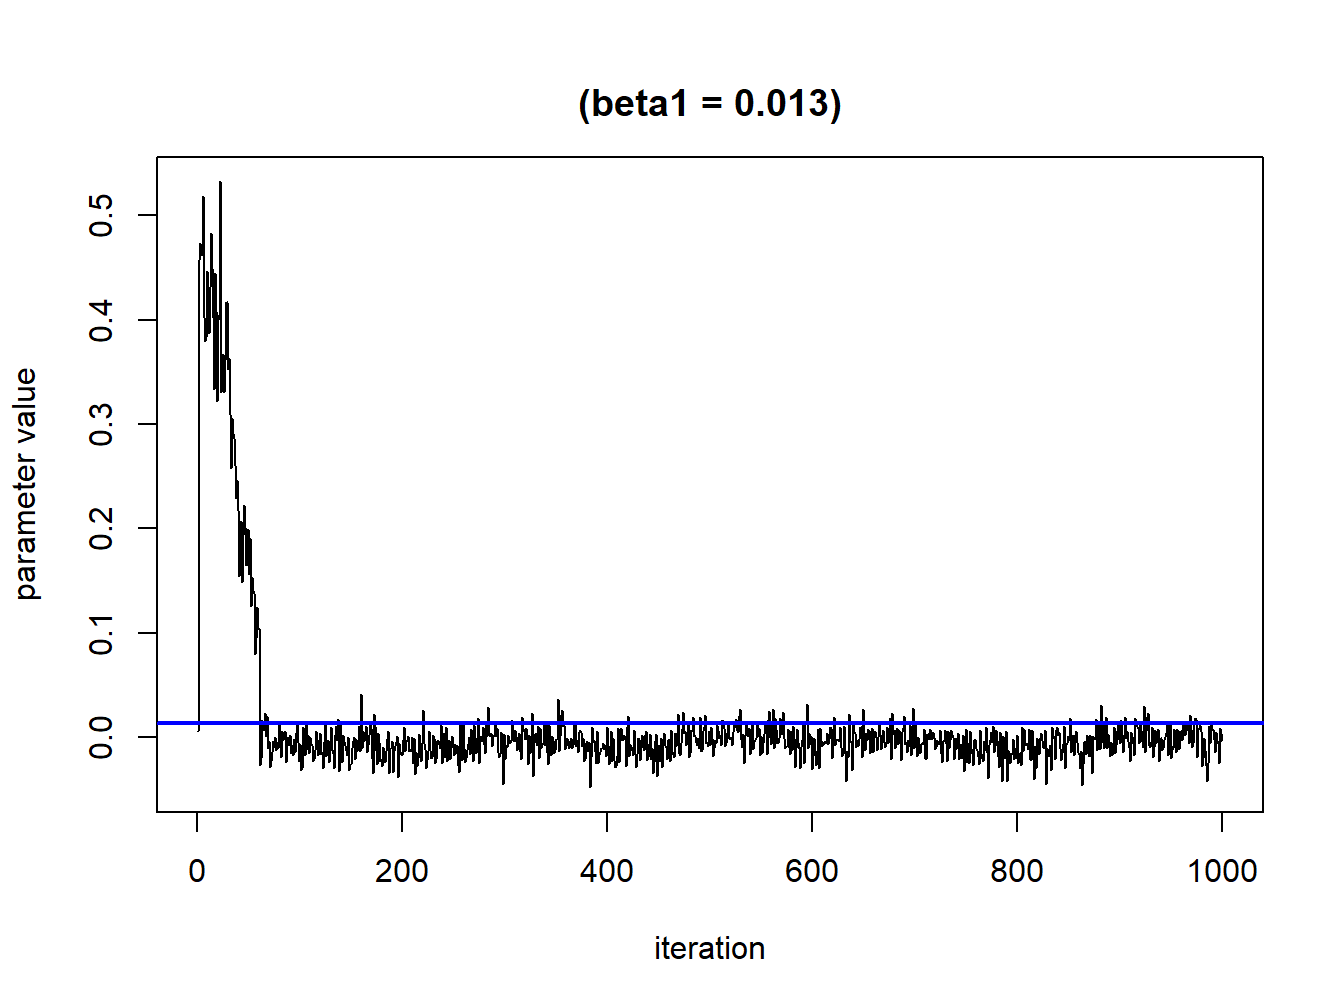
\includegraphics[width=0.8\linewidth]{bookdown-demo_files/figure-latex/figureenetadjs-1} 

}

\caption{Convergence plot for a single parameter without exclusions}\label{fig:figureenetadjs}
\end{figure}

\begin{Shaded}
\begin{Highlighting}[]
\NormalTok{sel}\OtherTok{\textless{}{-}}\FunctionTok{seq}\NormalTok{(}\DecValTok{100}\NormalTok{,}\DecValTok{1000}\NormalTok{,}\AttributeTok{by=}\DecValTok{1}\NormalTok{)}
\end{Highlighting}
\end{Shaded}

\begin{Shaded}
\begin{Highlighting}[]
\FunctionTok{TracePlot}\NormalTok{(}\AttributeTok{fit =}\NormalTok{ temp, }\AttributeTok{par =} \StringTok{"beta"}\NormalTok{, }\AttributeTok{sel=}\NormalTok{sel)}
\end{Highlighting}
\end{Shaded}

\begin{figure}[H]

{\centering 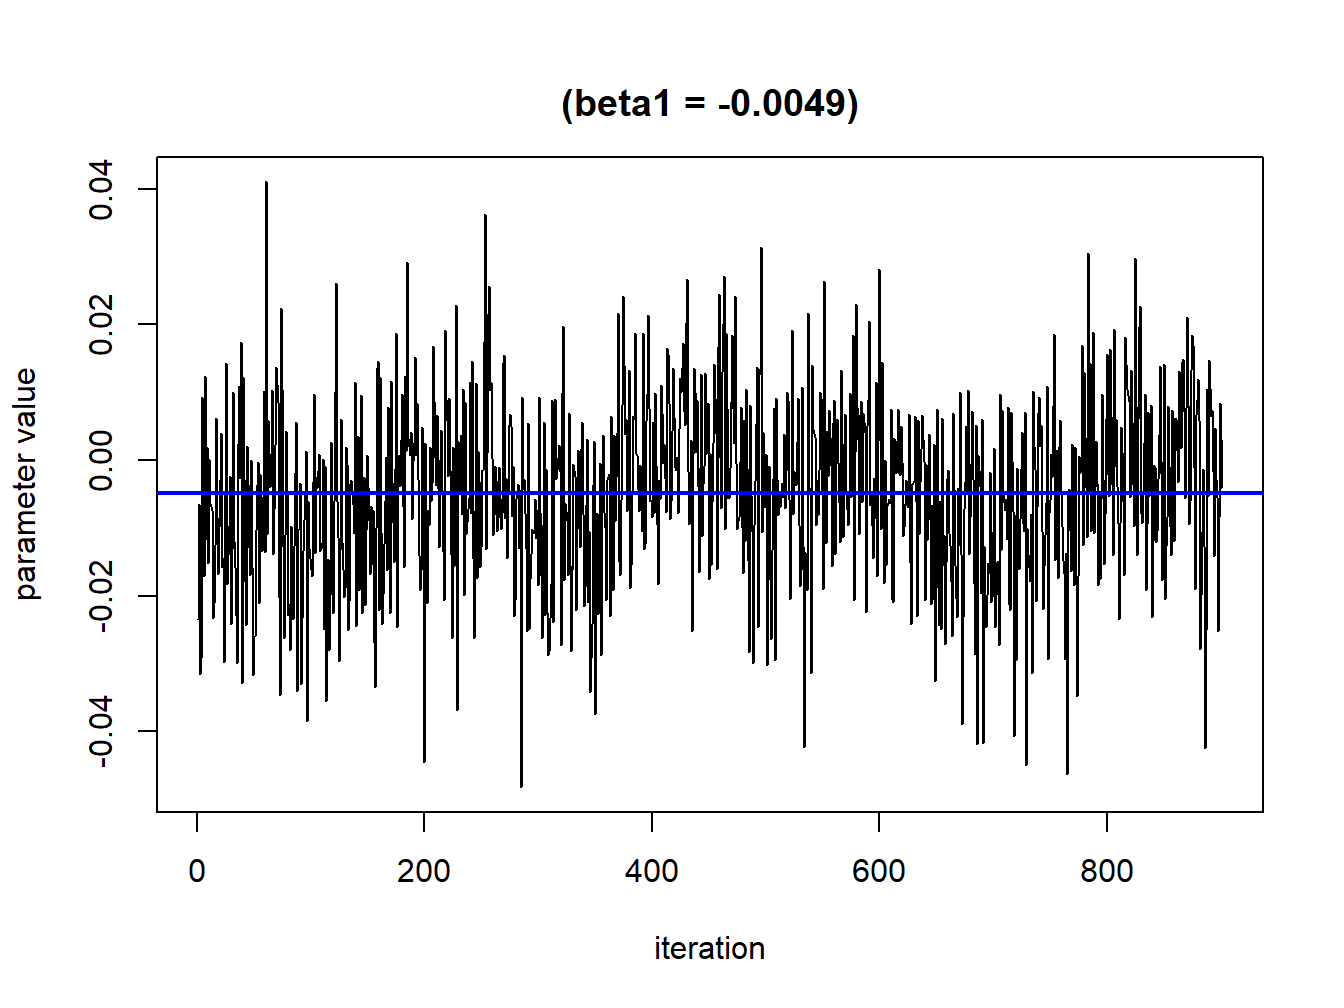
\includegraphics[width=0.8\linewidth]{bookdown-demo_files/figure-latex/figureenetadjsd-1} 

}

\caption{Convergence plot for a single parameter after burning phase exclusion}\label{fig:figureenetadjsd}
\end{figure}

\hypertarget{visualizing-results}{%
\subsection{Visualizing results}\label{visualizing-results}}

After estimation of a BKMR model, which is relatively straightforward and just requires patience throughout iterations, most of the work will consist of presenting post-estimation figures and functions that can present the complex relationship between the mixture and the outcome. The R package includes several functions to summarize the model output in different ways and to visually display the results.

To visualize the exposure-response functions we need to create different dataframes with the predictions that will be then graphically displayed with \texttt{ggpolot}.

\begin{Shaded}
\begin{Highlighting}[]
\NormalTok{pred.resp.univar }\OtherTok{\textless{}{-}} \FunctionTok{PredictorResponseUnivar}\NormalTok{(}\AttributeTok{fit =}\NormalTok{ temp, }\AttributeTok{sel=}\NormalTok{sel, }\AttributeTok{method=}\StringTok{"approx"}\NormalTok{)}

\NormalTok{pred.resp.bivar  }\OtherTok{\textless{}{-}} \FunctionTok{PredictorResponseBivar}\NormalTok{(}\AttributeTok{fit =}\NormalTok{ temp,  }\AttributeTok{min.plot.dist =} \DecValTok{1}\NormalTok{, }\AttributeTok{sel=}\NormalTok{sel, }
                                           \AttributeTok{method=}\StringTok{"approx"}\NormalTok{)}

\NormalTok{pred.resp.bivar.levels }\OtherTok{\textless{}{-}} \FunctionTok{PredictorResponseBivarLevels}\NormalTok{(}\AttributeTok{pred.resp.df =}\NormalTok{ pred.resp.bivar, }
                         \AttributeTok{Z =}\NormalTok{ mixture, }\AttributeTok{both\_pairs =} \ConstantTok{TRUE}\NormalTok{, }\AttributeTok{qs =} \FunctionTok{c}\NormalTok{(}\FloatTok{0.25}\NormalTok{, }\FloatTok{0.5}\NormalTok{, }\FloatTok{0.75}\NormalTok{))}

\NormalTok{risks.overall }\OtherTok{\textless{}{-}} \FunctionTok{OverallRiskSummaries}\NormalTok{(}\AttributeTok{fit =}\NormalTok{ temp, }\AttributeTok{qs =} \FunctionTok{seq}\NormalTok{(}\FloatTok{0.25}\NormalTok{, }\FloatTok{0.75}\NormalTok{, }\AttributeTok{by =} \FloatTok{0.05}\NormalTok{), }
                                      \AttributeTok{q.fixed =} \FloatTok{0.5}\NormalTok{, }\AttributeTok{method =} \StringTok{"approx"}\NormalTok{,}\AttributeTok{sel=}\NormalTok{sel)}

\NormalTok{risks.singvar }\OtherTok{\textless{}{-}} \FunctionTok{SingVarRiskSummaries}\NormalTok{(}\AttributeTok{fit =}\NormalTok{ temp, }\AttributeTok{qs.diff =} \FunctionTok{c}\NormalTok{(}\FloatTok{0.25}\NormalTok{, }\FloatTok{0.75}\NormalTok{),}
                                    \AttributeTok{q.fixed =} \FunctionTok{c}\NormalTok{(}\FloatTok{0.25}\NormalTok{, }\FloatTok{0.50}\NormalTok{, }\FloatTok{0.75}\NormalTok{), }\AttributeTok{method =} \StringTok{"approx"}\NormalTok{)}

\NormalTok{risks.int }\OtherTok{\textless{}{-}} \FunctionTok{SingVarIntSummaries}\NormalTok{(}\AttributeTok{fit =}\NormalTok{ temp, }\AttributeTok{qs.diff =} \FunctionTok{c}\NormalTok{(}\FloatTok{0.25}\NormalTok{, }\FloatTok{0.75}\NormalTok{),}
                                 \AttributeTok{qs.fixed =} \FunctionTok{c}\NormalTok{(}\FloatTok{0.25}\NormalTok{, }\FloatTok{0.75}\NormalTok{))}
\end{Highlighting}
\end{Shaded}

The first three objects will allow us to examine the predictor-response functions, while the next three objects will calculate a range of summary statistics that highlight specific features of the surface.

\hypertarget{univariate-dose-responses}{%
\subsubsection{Univariate dose-responses}\label{univariate-dose-responses}}

One cross section of interest is the univariate relationship between each covariate and the outcome, where all of the other exposures are fixed to a particular percentile. This can be done using the function \texttt{PredictorResponseUnivar}. The argument specifying the quantile at which to fix the other exposures is given by \texttt{q.fixed} (the default value is \texttt{q.fixed\ =\ 0.5}).

\begin{Shaded}
\begin{Highlighting}[]
\FunctionTok{ggplot}\NormalTok{(pred.resp.univar, }\FunctionTok{aes}\NormalTok{(z, est, }\AttributeTok{ymin =}\NormalTok{ est }\SpecialCharTok{{-}} \FloatTok{1.96}\SpecialCharTok{*}\NormalTok{se, }\AttributeTok{ymax =}\NormalTok{ est }\SpecialCharTok{+} \FloatTok{1.96}\SpecialCharTok{*}\NormalTok{se)) }\SpecialCharTok{+} 
  \FunctionTok{geom\_smooth}\NormalTok{(}\AttributeTok{stat =} \StringTok{"identity"}\NormalTok{) }\SpecialCharTok{+} \FunctionTok{ylab}\NormalTok{(}\StringTok{"h(z)"}\NormalTok{) }\SpecialCharTok{+} \FunctionTok{facet\_wrap}\NormalTok{(}\SpecialCharTok{\textasciitilde{}}\NormalTok{ variable) }
\end{Highlighting}
\end{Shaded}

\begin{figure}[H]

{\centering 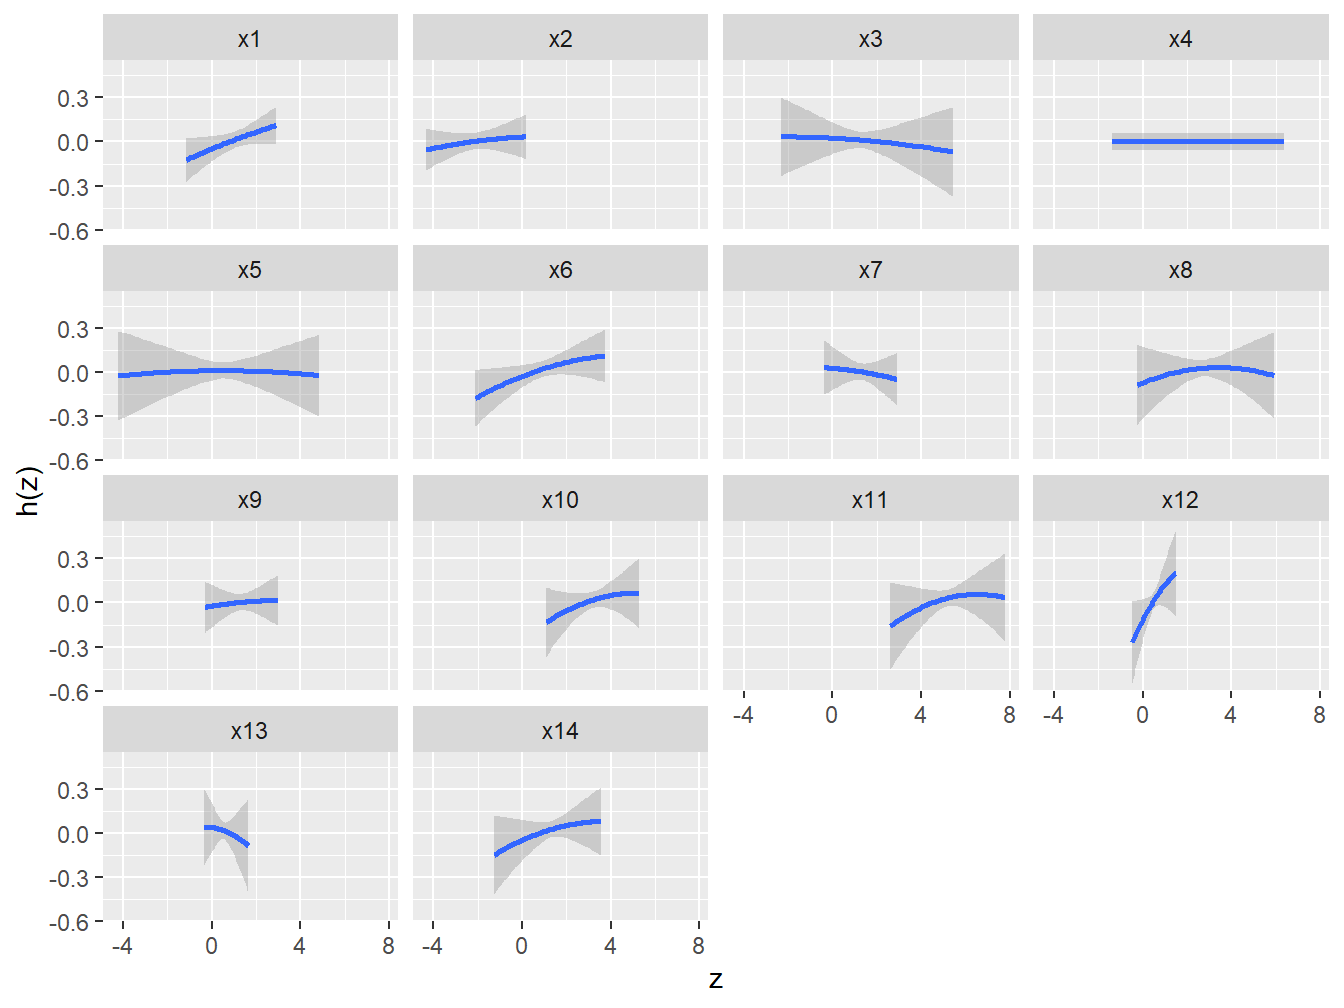
\includegraphics[width=0.8\linewidth]{bookdown-demo_files/figure-latex/save-1} 

}

\caption{Univariate dose-response associations from BKMR}\label{fig:save}
\end{figure}

We can conclude from these figures that all selected covariates have weak to moderate associations, and that all dose-responses seem to be linear (maybe leaving some benefit of doubt to \(X_6\)).

\hypertarget{bivariable-exposure-response-functions}{%
\subsubsection{Bivariable Exposure-Response Functions}\label{bivariable-exposure-response-functions}}

This visualizes the bivariate exposure-response function for two predictors, where all of the other predictors are fixed at a particular percentile.

\begin{Shaded}
\begin{Highlighting}[]
\FunctionTok{ggplot}\NormalTok{(pred.resp.bivar, }\FunctionTok{aes}\NormalTok{(z1, z2, }\AttributeTok{fill =}\NormalTok{ est)) }\SpecialCharTok{+} 
  \FunctionTok{geom\_raster}\NormalTok{() }\SpecialCharTok{+} 
  \FunctionTok{facet\_grid}\NormalTok{(variable2 }\SpecialCharTok{\textasciitilde{}}\NormalTok{ variable1) }\SpecialCharTok{+}
  \FunctionTok{scale\_fill\_gradientn}\NormalTok{(}\AttributeTok{colours=}\FunctionTok{c}\NormalTok{(}\StringTok{"\#0000FFFF"}\NormalTok{,}\StringTok{"\#FFFFFFFF"}\NormalTok{,}\StringTok{"\#FF0000FF"}\NormalTok{)) }\SpecialCharTok{+}
  \FunctionTok{xlab}\NormalTok{(}\StringTok{"expos1"}\NormalTok{) }\SpecialCharTok{+}
  \FunctionTok{ylab}\NormalTok{(}\StringTok{"expos2"}\NormalTok{) }\SpecialCharTok{+}
  \FunctionTok{ggtitle}\NormalTok{(}\StringTok{"h(expos1, expos2)"}\NormalTok{)}
\end{Highlighting}
\end{Shaded}

\begin{figure}[H]

{\centering 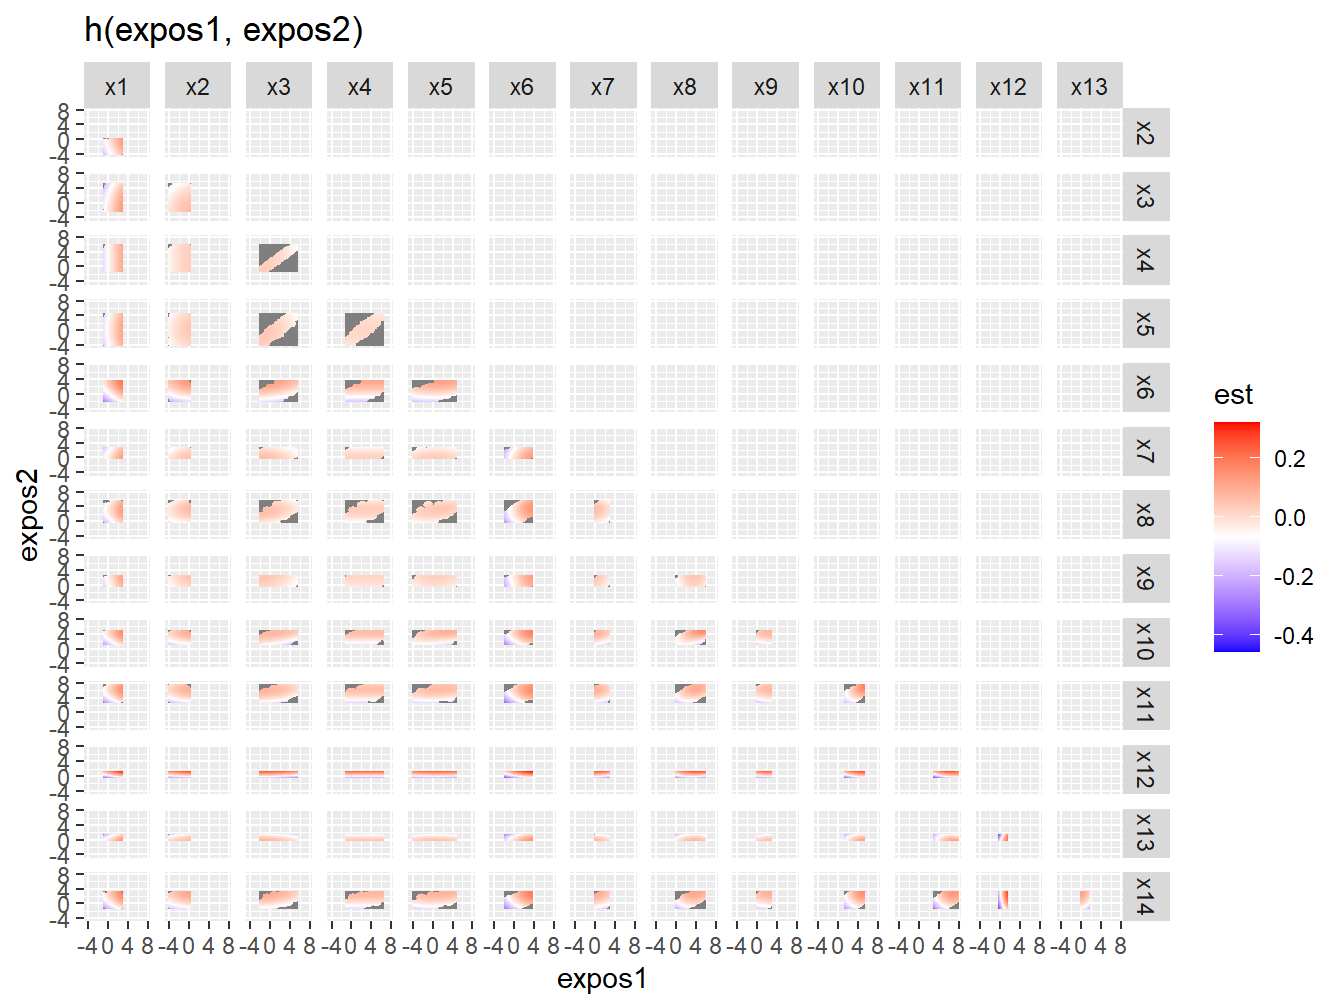
\includegraphics[width=0.8\linewidth]{bookdown-demo_files/figure-latex/save2-1} 

}

\caption{Bivariate exposure-response associations from BKMR}\label{fig:save2}
\end{figure}

\hypertarget{interactions}{%
\subsubsection{Interactions}\label{interactions}}

The figure we just plotted might not be the most intuitive way of checking for interactions. An alternative approach is to investigate the predictor-response function of a single predictor in Z for the second predictor in Z fixed at various quantiles (and for the remaining predictors fixed to a particular value). These can be obtained using the \texttt{PredictorResponseBivarLevels} function, which takes as input the bivariate exposure-response function outputted from the previous command, where the argument \texttt{qs} specifies a sequence of quantiles at which to fix the second predictor. We can easily select a specific combination we want to present, like the X6-X12 one.

\begin{Shaded}
\begin{Highlighting}[]
\FunctionTok{ggplot}\NormalTok{(pred.resp.bivar.levels, }\FunctionTok{aes}\NormalTok{(z1, est)) }\SpecialCharTok{+} 
  \FunctionTok{geom\_smooth}\NormalTok{(}\FunctionTok{aes}\NormalTok{(}\AttributeTok{col =}\NormalTok{ quantile), }\AttributeTok{stat =} \StringTok{"identity"}\NormalTok{) }\SpecialCharTok{+} 
 \FunctionTok{facet\_grid}\NormalTok{(variable2 }\SpecialCharTok{\textasciitilde{}}\NormalTok{ variable1) }\SpecialCharTok{+}
  \FunctionTok{ggtitle}\NormalTok{(}\StringTok{"h(expos1 | quantiles of expos2)"}\NormalTok{) }\SpecialCharTok{+}
 \FunctionTok{xlab}\NormalTok{(}\StringTok{"expos1"}\NormalTok{)}
\end{Highlighting}
\end{Shaded}

\begin{figure}[H]

{\centering 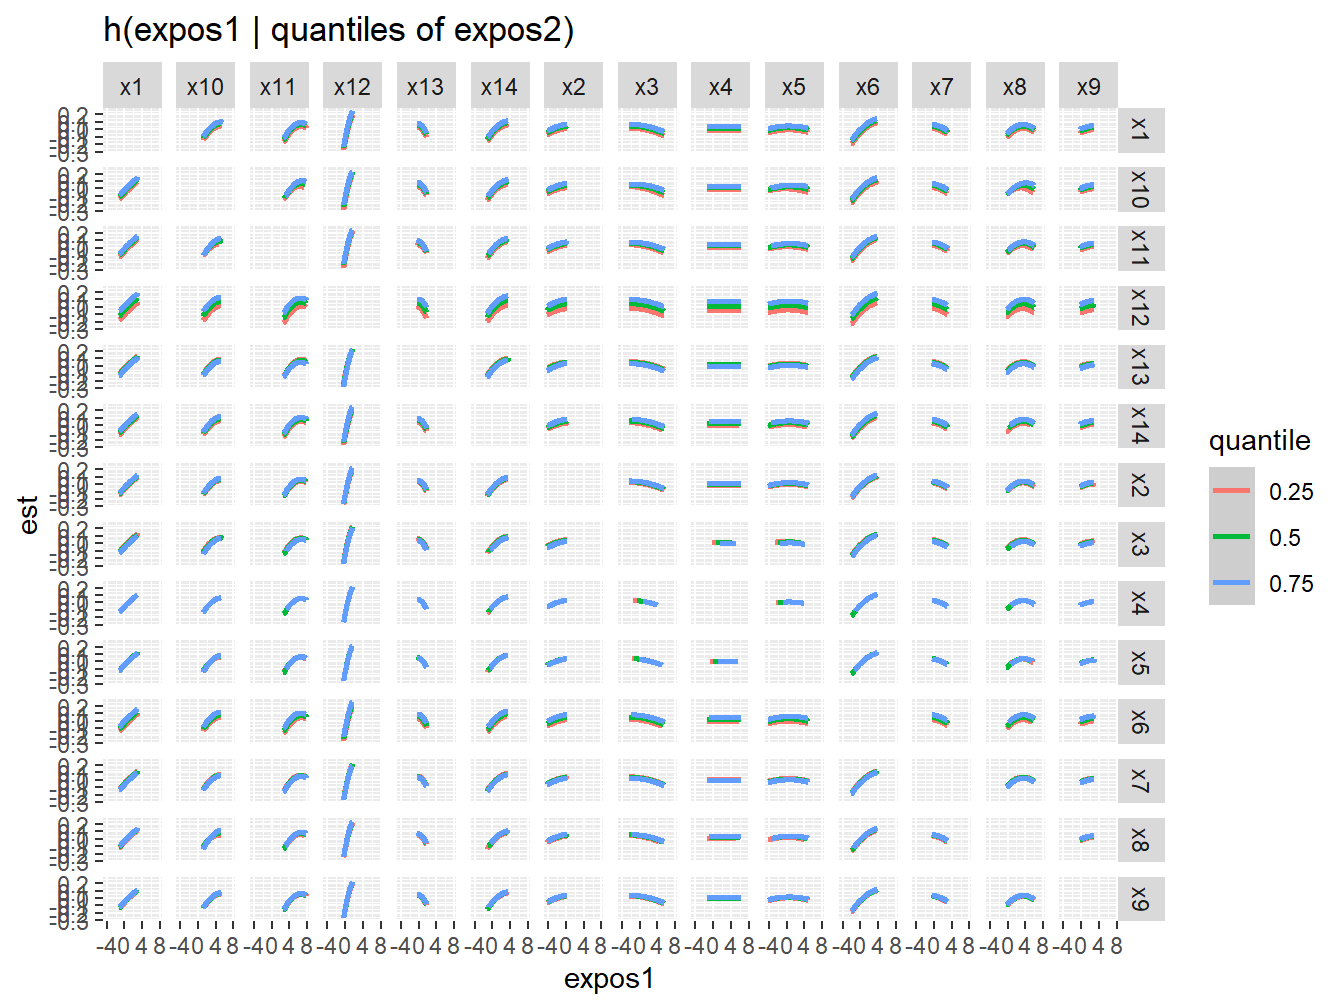
\includegraphics[width=0.8\linewidth]{bookdown-demo_files/figure-latex/save3-1} 

}

\caption{Qualitative interaction assessment from BKMR}\label{fig:save3}
\end{figure}

\begin{figure}[H]

{\centering 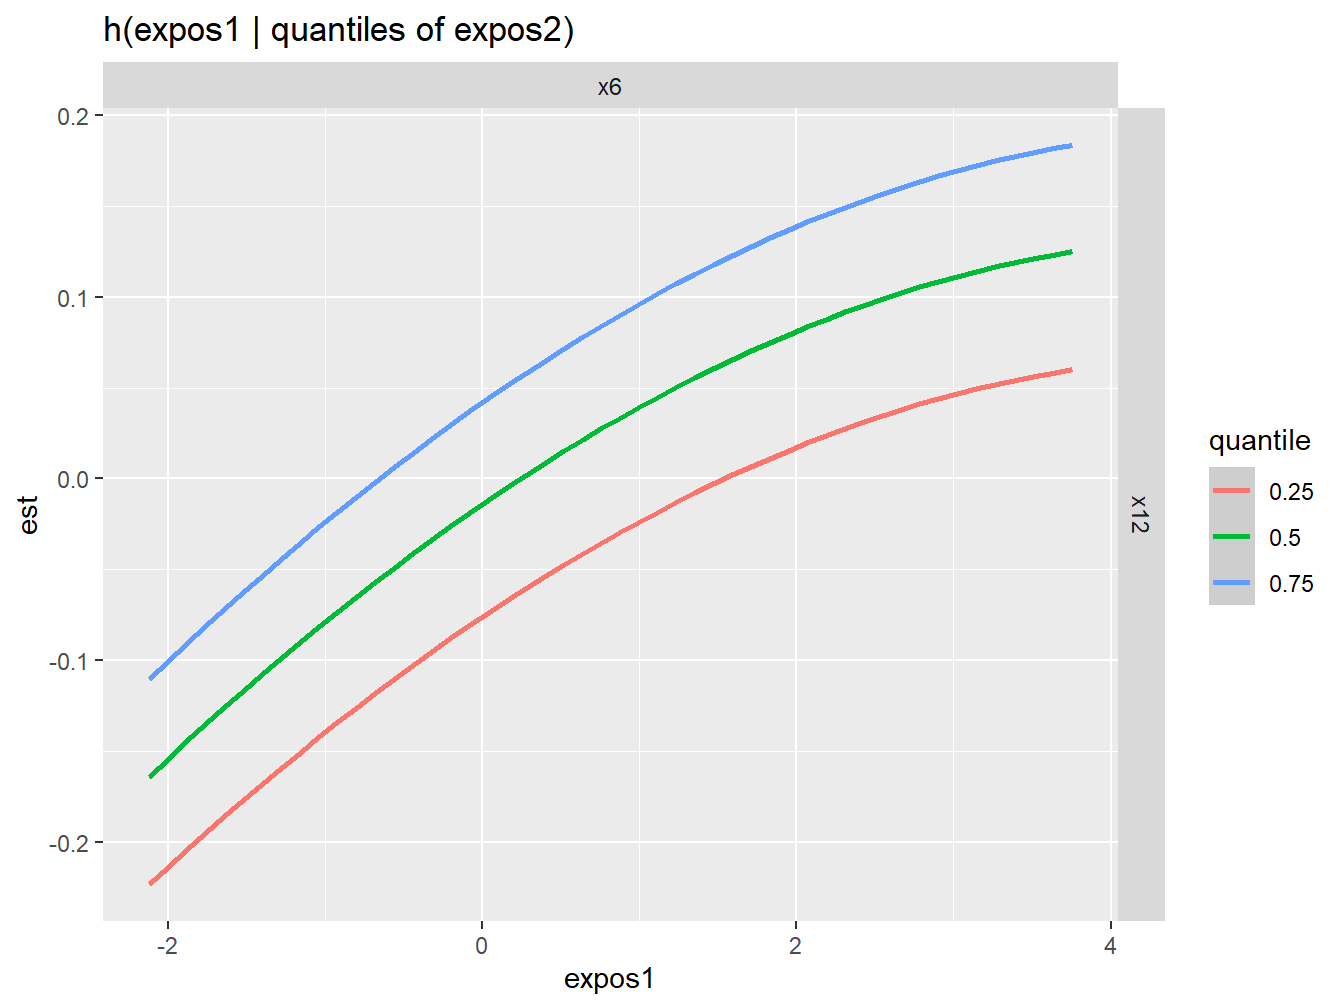
\includegraphics[width=0.8\linewidth]{bookdown-demo_files/figure-latex/save3fdg-1} 

}

\caption{Qualitative interaction assessment between X6 and x12 from BKMR}\label{fig:save3fdg}
\end{figure}

This figures do not provide any evidence of interactions throughout the mixture.

\hypertarget{overall-mixture-effect}{%
\subsubsection{Overall Mixture Effect}\label{overall-mixture-effect}}

Another interesting summary plot is the overall effect of the mixture, calculated by comparing the value of \(h\) when all of predictors are at a particular percentile as compared to when all of them are at their 50th percentile. The function \texttt{OverallRiskSummaries} allows one to specify a sequence of values of quantiles using the argument \texttt{qs} and the fixed quantile (the default is the 50th percentile) using the argument \texttt{q.fixed}.

\begin{Shaded}
\begin{Highlighting}[]
\FunctionTok{ggplot}\NormalTok{(risks.overall, }\FunctionTok{aes}\NormalTok{(quantile, est, }\AttributeTok{ymin =}\NormalTok{ est }\SpecialCharTok{{-}} \FloatTok{1.96}\SpecialCharTok{*}\NormalTok{sd, }\AttributeTok{ymax =}\NormalTok{ est }\SpecialCharTok{+} \FloatTok{1.96}\SpecialCharTok{*}\NormalTok{sd)) }\SpecialCharTok{+}  
  \FunctionTok{geom\_hline}\NormalTok{(}\AttributeTok{yintercept=}\DecValTok{00}\NormalTok{, }\AttributeTok{linetype=}\StringTok{"dashed"}\NormalTok{, }\AttributeTok{color=}\StringTok{"gray"}\NormalTok{) }\SpecialCharTok{+} 
  \FunctionTok{geom\_pointrange}\NormalTok{() }\SpecialCharTok{+} \FunctionTok{scale\_y\_continuous}\NormalTok{(}\AttributeTok{name=}\StringTok{"estimate"}\NormalTok{) }
\end{Highlighting}
\end{Shaded}

\begin{figure}[H]

{\centering 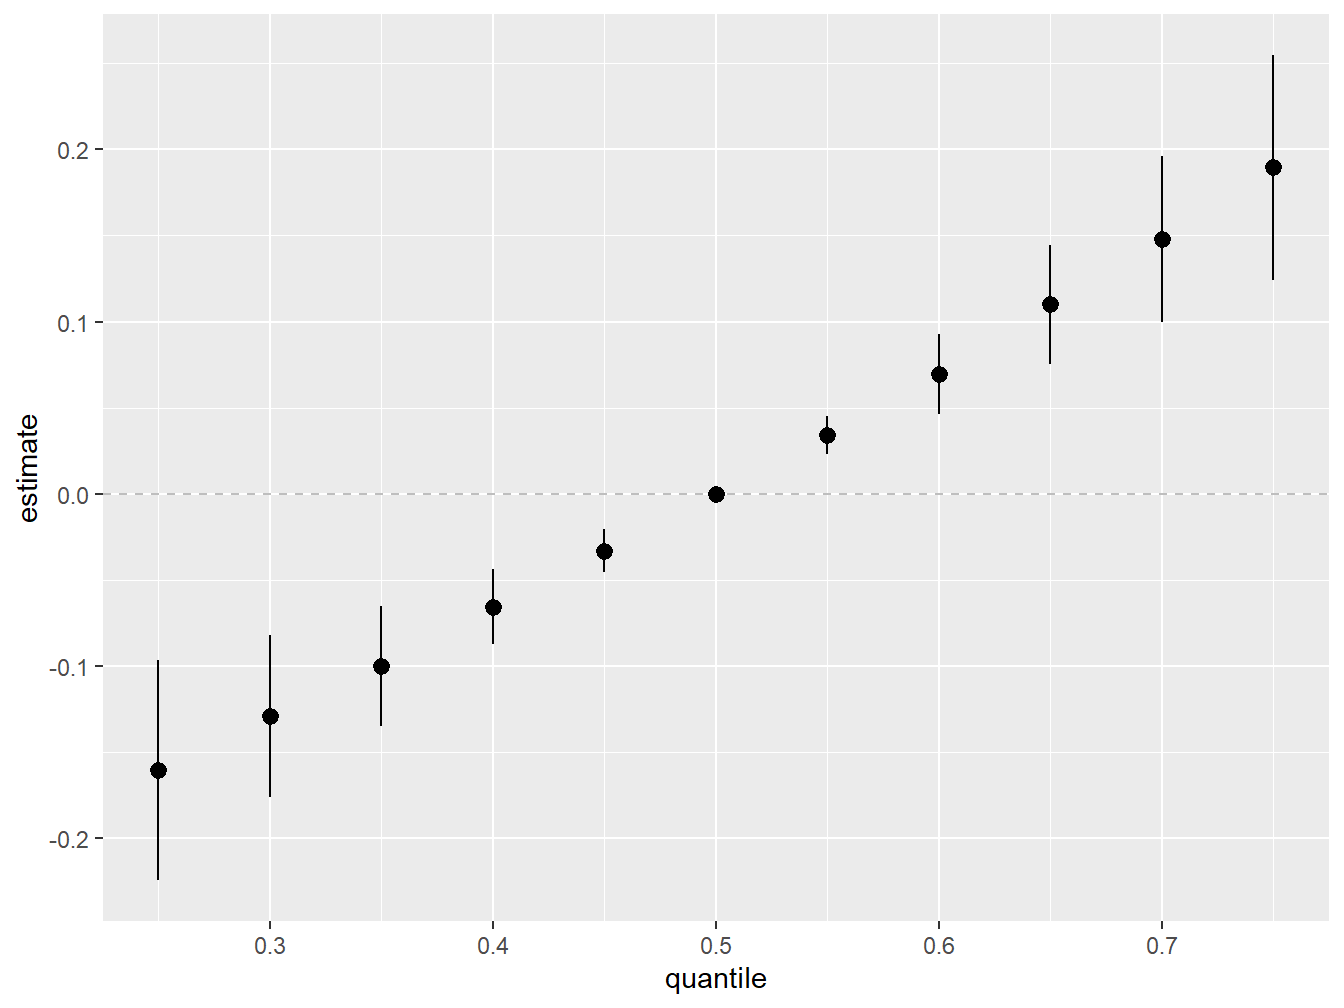
\includegraphics[width=0.8\linewidth]{bookdown-demo_files/figure-latex/save4-1} 

}

\caption{Overall Mixture Effect from BKMR}\label{fig:save4}
\end{figure}

In agreement with WQS, higher exposure to the overall mixture is associated with higher mean outcome.

\hypertarget{single-variables-effects}{%
\subsubsection{Single Variables effects}\label{single-variables-effects}}

This additional function summarizes the contribution of an individual predictor to the response. For example, we may wish to compare risk when a single predictor in \(h\) is at the 75th percentile as compared to when that predictor is at its 25th percentile, where we fix all of the remaining predictors to a particular percentile.

\begin{Shaded}
\begin{Highlighting}[]
\FunctionTok{ggplot}\NormalTok{(risks.singvar, }\FunctionTok{aes}\NormalTok{(variable, est, }\AttributeTok{ymin =}\NormalTok{ est }\SpecialCharTok{{-}} \FloatTok{1.96}\SpecialCharTok{*}\NormalTok{sd,  }\AttributeTok{ymax =}\NormalTok{ est }\SpecialCharTok{+} \FloatTok{1.96}\SpecialCharTok{*}\NormalTok{sd, }
       \AttributeTok{col =}\NormalTok{ q.fixed)) }\SpecialCharTok{+} \FunctionTok{geom\_hline}\NormalTok{(}\FunctionTok{aes}\NormalTok{(}\AttributeTok{yintercept=}\DecValTok{0}\NormalTok{), }\AttributeTok{linetype=}\StringTok{"dashed"}\NormalTok{, }
       \AttributeTok{color=}\StringTok{"gray"}\NormalTok{) }\SpecialCharTok{+}  \FunctionTok{geom\_pointrange}\NormalTok{(}\AttributeTok{position =} \FunctionTok{position\_dodge}\NormalTok{(}\AttributeTok{width =} \FloatTok{0.75}\NormalTok{)) }\SpecialCharTok{+}
       \FunctionTok{coord\_flip}\NormalTok{() }\SpecialCharTok{+} \FunctionTok{theme}\NormalTok{(}\AttributeTok{legend.position=}\StringTok{"none"}\NormalTok{)}\SpecialCharTok{+}\FunctionTok{scale\_x\_discrete}\NormalTok{(}\AttributeTok{name=}\StringTok{""}\NormalTok{) }\SpecialCharTok{+}
       \FunctionTok{scale\_y\_continuous}\NormalTok{(}\AttributeTok{name=}\StringTok{"estimate"}\NormalTok{) }
\end{Highlighting}
\end{Shaded}

\begin{figure}[H]

{\centering 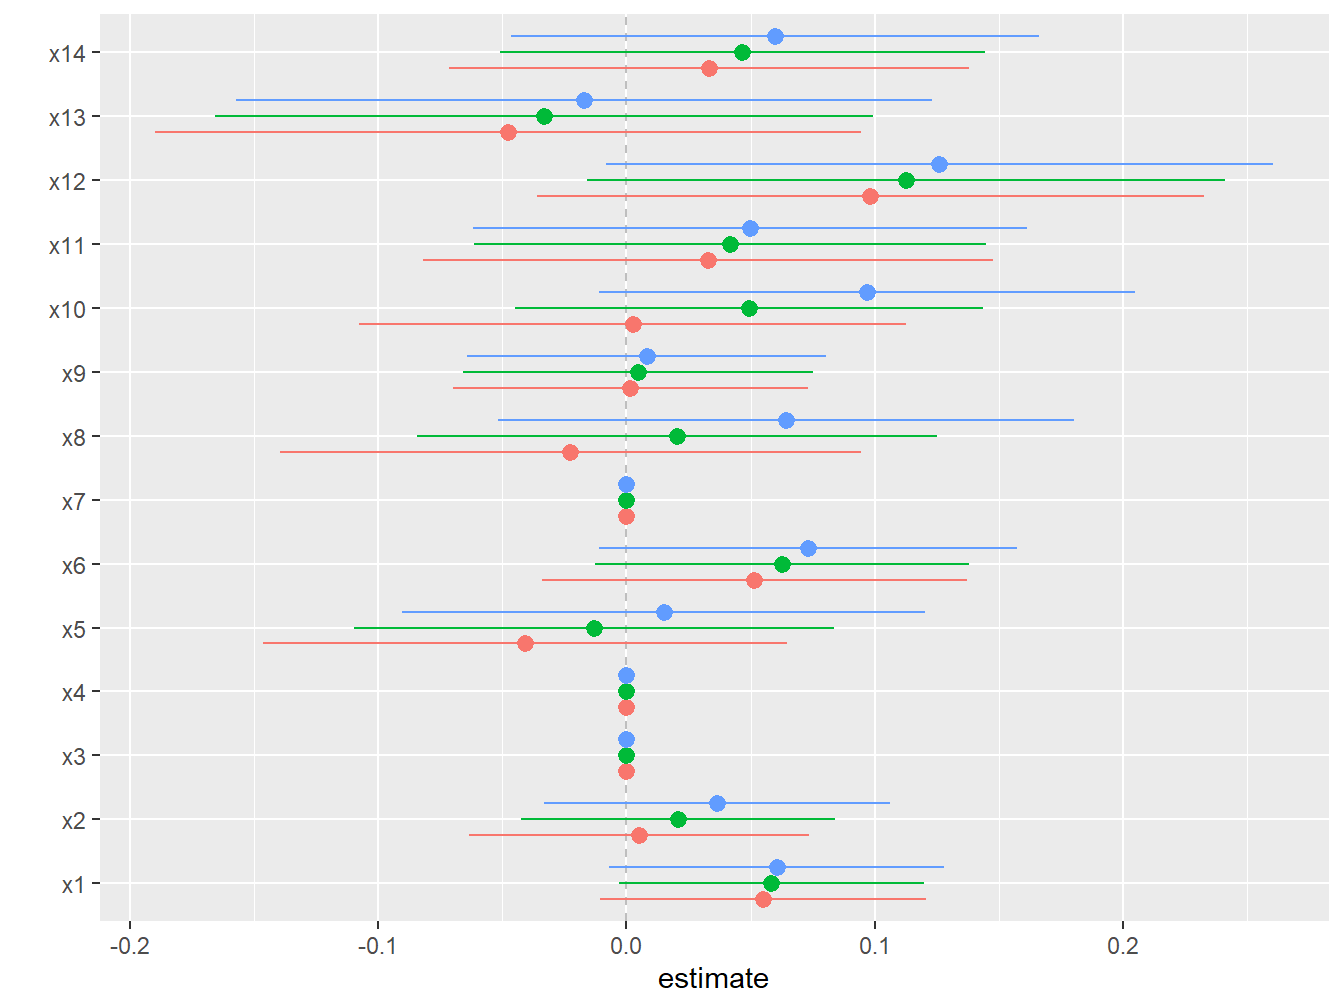
\includegraphics[width=0.8\linewidth]{bookdown-demo_files/figure-latex/save5-1} 

}

\caption{Individual effects from BKMR}\label{fig:save5}
\end{figure}

\hypertarget{single-variable-interaction-terms}{%
\subsubsection{Single Variable Interaction Terms}\label{single-variable-interaction-terms}}

Finally, this function is similar to the latest one, but refers to the interaction of a single exposure with all other covariates. It attempts to represent an overall interaction between that exposure and all other components.

\begin{Shaded}
\begin{Highlighting}[]
\FunctionTok{ggplot}\NormalTok{(risks.int, }\FunctionTok{aes}\NormalTok{(variable, est, }\AttributeTok{ymin =}\NormalTok{ est }\SpecialCharTok{{-}} \FloatTok{1.96}\SpecialCharTok{*}\NormalTok{sd, }\AttributeTok{ymax =}\NormalTok{ est }\SpecialCharTok{+} \FloatTok{1.96}\SpecialCharTok{*}\NormalTok{sd)) }\SpecialCharTok{+} 
  \FunctionTok{geom\_pointrange}\NormalTok{(}\AttributeTok{position =} \FunctionTok{position\_dodge}\NormalTok{(}\AttributeTok{width =} \FloatTok{0.75}\NormalTok{)) }\SpecialCharTok{+} 
  \FunctionTok{geom\_hline}\NormalTok{(}\AttributeTok{yintercept =} \DecValTok{0}\NormalTok{, }\AttributeTok{lty =} \DecValTok{2}\NormalTok{, }\AttributeTok{col =} \StringTok{"brown"}\NormalTok{) }\SpecialCharTok{+} \FunctionTok{coord\_flip}\NormalTok{()}
\end{Highlighting}
\end{Shaded}

\begin{figure}[H]

{\centering 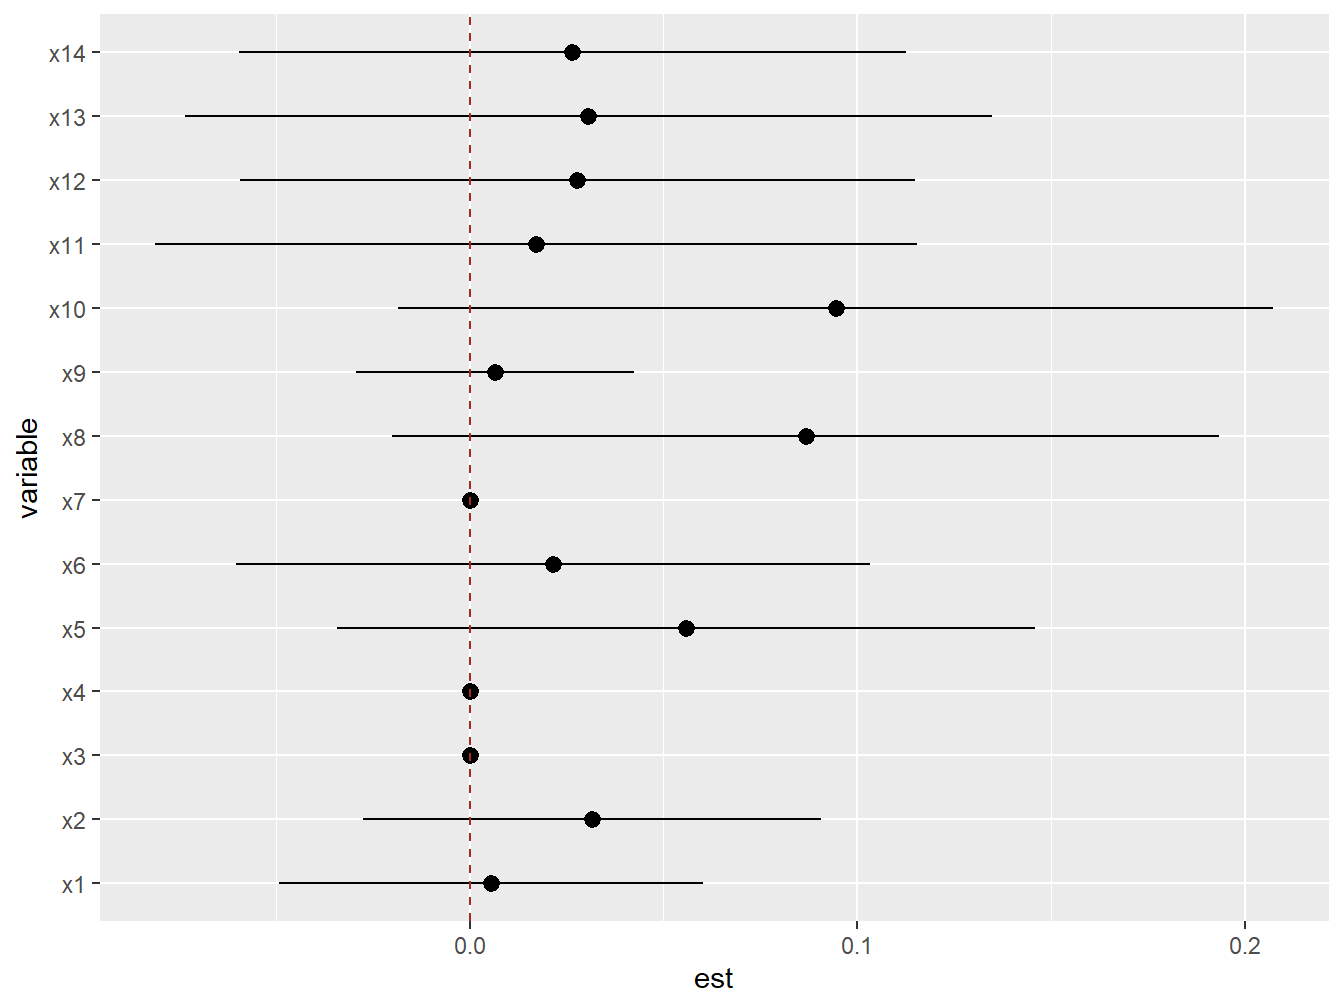
\includegraphics[width=0.8\linewidth]{bookdown-demo_files/figure-latex/save6-1} 

}

\caption{Individual interaction effects from BKMR}\label{fig:save6}
\end{figure}

As we concluded before, this graph also leads us to conclude that we have no evidence of interaction for any covariate (which, as we know from simulated data, is true).

\hypertarget{hierarchical-selection}{%
\subsection{Hierarchical selection}\label{hierarchical-selection}}

The variable selection procedure embedded into BKMR can also operate within a hierarchical procedure. Using our example, we could for instance inform the model that there are highly correlated clusters of exposures. This will allow us to get an estimate of the relative importance of each cluster and of each exposure within it. The procedure is implemented as follows, where we are specifically informing the model that there is a cluster of three highly correlated covariates:

\begin{Shaded}
\begin{Highlighting}[]
\NormalTok{hier }\OtherTok{\textless{}{-}}  \FunctionTok{kmbayes}\NormalTok{(}\AttributeTok{y=}\NormalTok{y, }\AttributeTok{Z=}\NormalTok{mixture, }\AttributeTok{X=}\NormalTok{covariates, }\AttributeTok{iter=}\DecValTok{1000}\NormalTok{, }\AttributeTok{verbose=}\ConstantTok{FALSE}\NormalTok{, }\AttributeTok{varsel=}\ConstantTok{TRUE}\NormalTok{, }
                 \AttributeTok{knots=}\NormalTok{knots100, }\AttributeTok{groups=}\FunctionTok{c}\NormalTok{(}\DecValTok{1}\NormalTok{,}\DecValTok{1}\NormalTok{,}\DecValTok{2}\NormalTok{,}\DecValTok{2}\NormalTok{,}\DecValTok{2}\NormalTok{,}\DecValTok{1}\NormalTok{,}\DecValTok{1}\NormalTok{,}\DecValTok{1}\NormalTok{,}\DecValTok{1}\NormalTok{,}\DecValTok{1}\NormalTok{,}\DecValTok{1}\NormalTok{,}\DecValTok{1}\NormalTok{,}\DecValTok{1}\NormalTok{,}\DecValTok{1}\NormalTok{))}

\FunctionTok{ExtractPIPs}\NormalTok{(hier)}
\end{Highlighting}
\end{Shaded}

\begin{verbatim}
##    variable group groupPIP   condPIP
## 1        x1     1    1.000 0.0000000
## 2        x2     1    1.000 0.0000000
## 3        x3     2    0.044 0.3636364
## 4        x4     2    0.044 0.4545455
## 5        x5     2    0.044 0.1818182
## 6        x6     1    1.000 0.0160000
## 7        x7     1    1.000 0.0040000
## 8        x8     1    1.000 0.0620000
## 9        x9     1    1.000 0.0540000
## 10      x10     1    1.000 0.0000000
## 11      x11     1    1.000 0.0020000
## 12      x12     1    1.000 0.4500000
## 13      x13     1    1.000 0.1460000
## 14      x14     1    1.000 0.2660000
\end{verbatim}

Group PIPs seem to point out that the cluster is somehow relevant in the dose-response association, and indicates that that \(X_4\) might be the most relevant of the three exposures.

\hypertarget{extensions}{%
\subsection{Extensions}\label{extensions}}

The first release of BKMR was only available for evaluating continuous outcomes, but recent work has extended its use to the context of binary outcomes, which are also integrated in the latest versions of the package. \citet{domingo2019association} have also described how to apply BKMR with time-to-event outcomes. Additional extensions of the approach that could be of interest in several settings also include a longitudinal version of BKMR based on lagged regression, which can be used to evaluate time-varying mixtures (\citet{liu2018lagged}). While this method is not yet implemented in the package, it is important to note that similar results can be achieved by evaluating time-varying effects through hierarchical selection. In brief, multiple measurements of exposures can be included simultaneously in the kernel, grouping exposures by time. An example of this application can be found in \citet{tyagi2021identifying}, evaluating exposures to phthalates during pregnancy, measured at different trimester, as they relate to final gestational weight. By providing a measure of group importance, group PIPs can here be interpreted as measures of relative importance of the time-windows of interest, thus allowing a better understanding of the timing of higher susceptibility to mixture exposures.

Finally, we have described how BKMR can provide a graphical qualitative assessment of interaction. Some additional work is being conducted to formally provide measures of interaction and is briefly presented \href{https://github.com/jantonelli111/NLinteraction}{here}.

\hypertarget{practical-considerations-and-discussion}{%
\subsection{Practical considerations and discussion}\label{practical-considerations-and-discussion}}

To conclude our presentation of BKMR, let's list some useful considerations that one should take into account when applying this methodology:

\begin{itemize}
\tightlist
\item
  As a Bayesian technique, prior information could be specified on the model parameters. Nevertheless this is not commonly done, and all code presented here is assuming the use of non-informative priors. In general, it is good to remember that PIP values can be sensitive to priors (although relative importance tends to be stable).
\item
  Because of their sensitivity, PIP values can only be interpreted as a relative measure of importance (as ranking the importance of exposures). Several applied papers have been using thresholds (e.g.~0.5) to define a variable ``important'' but this is interpretation is erroneous and misleading.
\item
  The BKMR algorithm is more stable when it isn't dealing with exposures on vastly different scales. We typically center and scale both the outcome and the exposures (and continuous confounders). Similarly, we should be wary of exposure outliers, and log-transforming exposures is also recommended.
\item
  BKMR is operating a variable selection procedure. As such, a PIP of 0 will imply that the dose-response for that covariate is a straight line on zero. This does not mean that a given exposure has no effect on the outcome, but simply that it was not selected in the procedure. As a matter of fact, when an exposure has a weak effect on the outcome BKMR will mostly tend to exclude it. As a consequence of this, the overall mixture effect will really present the overall effect of the selected exposures.
\item
  As a Bayesian technique, BKMR is not based on the classical statistical framework on null-hypothesis testing. 95\% CI are interpreted as credible intervals, and common discussions on statistical power should be avoided.
\item
  Despite the estimation improvements through the use of knots as previously described, fitting a BKMR model remains time-demanding. In practice, you might be able to fit a BKMR model on a dataset of up to 10.000 individuals (still waiting few hours to get your results). For any large dataset, alternative approaches should be considered.
\item
  BKMR is a flexible non-parametric method that is designed to deal with complex settings with non-linearities and interactions. In standard settings, regression methods could provide a better estimation and an easier interpretation of results. In practical terms, you would never begin your analysis by fitting a BKMR model but only get to it for results validation or if alternative techniques were not sufficiently equipped to deal with your data.
\end{itemize}

\hypertarget{assessing-interactions}{%
\section{Assessing interactions}\label{assessing-interactions}}

\hypertarget{tree-based-modeling}{%
\subsection{Tree-based modeling}\label{tree-based-modeling}}

In settings when one is interested in formally evaluating interactions, unique challenges are involved. First, we already discussed how evaluating several covariates and high-order interactions within a regression framework
will rapidly increase the number of parameters to be estimated, and the
resulting complexity of the model will make classical regression techniques
of little use. Summary and classification approaches like WQS will not be able to provide an estimate of interaction effects, and we have just discussed how BKMR can only provide some qualitative assessment of interactions, and only among those exposures that have passed the selection procedure.

To account for the complexity of joint effects and high-dimensional interactions, one should consider specific techniques that have been specifically develop to deal with complex and big data. One machine learning (ML) approach that can be useful in the context of interaction analysis, and specifically when evaluating environmental exposures, is the application of boosted regression trees (BRT), BRT is a tree-based modeling technique that can be used to evaluate complex high-dimensional interactions
among several variables, which can be continuous, categorical, or binary. Boosted trees are
designed to improve the performance of classification and regression
trees (CARTs), which partition the data into several disjoint regions
approximating the outcome as constant within these regions. CARTs can
account for complex interactions by conditioning subsequent splits on
previous ones, a feature that is controlled by a ``depth'' option.
Higher-order depths correspond to accounting for higher-order interactions. In practical terms, this implies that by modifying the depth option of the algorithm we can incorporate an increasingly higher number of interaction orders. How many interactions should be evaluated, together with other parameters of the model, are identified by the machine through cross validation techniques.

Boosted trees improve the predictive performance of a single
CART by combining several weak learners to accurately identify a set of
explanatory variables that are associated with the outcome. The
improved predictive performance, however, will come at the expense of an easy
interpretation. Specifically, the output of a BRT will provide identification
of variable importance, partial dependence plot, and interactions
hierarchy, but will not provide effect estimates for
each variable or interaction as in classical regression. A BRT model will provide the following objects as output:

\begin{itemize}
\item
  Variable importance: this is based on how many times each variable is
  involved in a split, capturing its independent predictive power with
  respect to the outcome. This measure holds the same interpretation of PIPs in BKMR
\item
  Dependence plots: similarly to the univariate dose-responses in BKMR, these provide a graphical visualization
  of the fitted function that presents the associations between one
  or more predictors and the outcome. These plots are especially helpful
  with continuous predictors, but let's stress that this technique can be used with any kind of exposures.
\item
  H-statistics: these are the unique measures of interaction relevance, which indicate,
  for any pair of predictors, the fraction of variance that is not captured by
  the sum of the two fitted response functions. Of importance, the
  Depending on the depth of the algorithm, H-statistics can be calculated
  for all levels of interactions including 2-way and more. These measures
  do not provide a summary of relative importance (i.e.~they do not sum
  up to 1) but rather indicate a ranking of importance of interactions.
\end{itemize}

For more details on boosted trees we refer to previous publications (\citet{lampa2014identification}) and \href{http://uc-r.github.io/gbm_regression}{online documentation}.

In this study, parameters in the final
model were selected using a 10-fold cross validation on 75\% of the data
(training sample), estimating the model separately among men and
women, and selecting the model with the lowest root mean squared
error (RMSE).

\hypertarget{interaction-screening-and-regression-approaches}{%
\subsection{Interaction screening and regression approaches}\label{interaction-screening-and-regression-approaches}}

Let us stress once more that both BKMR, which provide a qualitative graphical assessment of interactions, and BRT models, which allow estimating H-statistics to rank interactions of different orders, do not provide direct estimates or tests for interactions effects. For this reason, a recommended practice is to use these techniques as interaction screening procedures and employ a 2-steps approach in which selected interactions are then evaluated in a final regression model. As an illustrative example, we used this approach in a recent paper to identify 2-ways interactions between occupational exposures and health factors that we later integrated in a regression models evaluating the effect of this mixture on ALS risk (\citet{bellavia2021joint}).

\begin{figure}
\centering
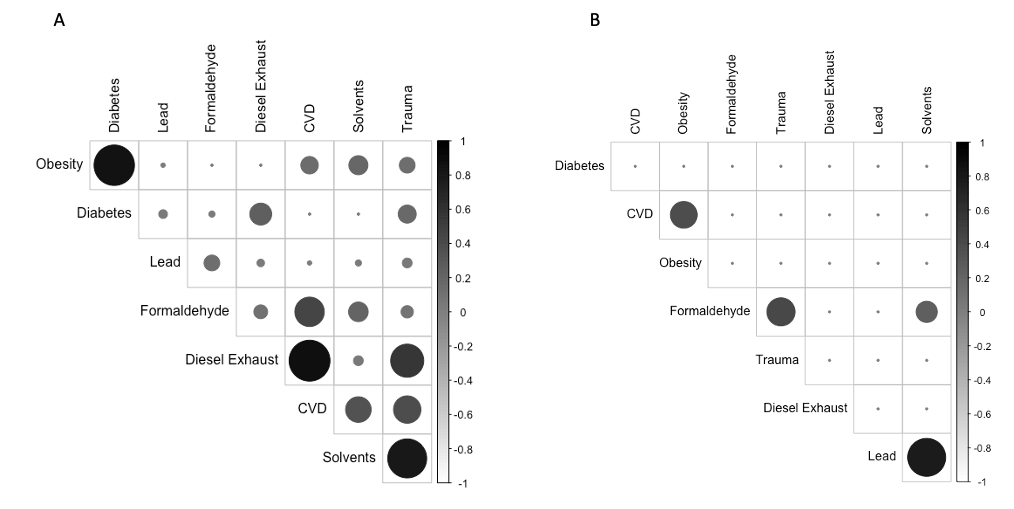
\includegraphics{images/hstats.png}
\caption{H-statistics from Bellavia et al.}
\end{figure}

\hypertarget{additional-topics-and-final-remarks}{%
\chapter{Additional topics and final remarks}\label{additional-topics-and-final-remarks}}

The aim of this last section is to provide a very brief introduction to additional topics that are often of relevance when investigating the health effects of multiple environmental exposures. First, we will provide a general overview of the extent to which what has been discussed so far can be evaluated from a causal inference perspective. Next, we will describe some relatively common situations where additional methodological considerations are required, namely the presence of zero-inflated or binary exposures. Finally, we will present an introductory overview of approaches that allow incorporating multiple exposures in mediation analysis, which is often a primary goal of exposome research.

\hypertarget{causal-mixture-effects}{%
\section{Causal mixture effects}\label{causal-mixture-effects}}

To improve our understanding of the associations between environmental exposures and health outcomes, and facilitate the development of more stringent public health regulations and interventions, it is important to determine to which extent these associations reflect causal relationships. To establish causal links, researchers are advocating the use of a pluralistic approach in terms of study design, to reduce the potential harm due to typical epidemiological bias such as confounding or selection bias, as well in terms of statistical methodologies for causal inference (\citet{vandenbroucke2016causality}), (\citet{dominici2017best}). In the specific case of environmental exposures, this switch from association to causation has to account for the co-occurrence of multiple components or constituents, present in the real world as a complex mixture. At this time, regulatory policies are still mostly designed to regulate one pollutant or chemical at the time, thus hampering the implementation of integrated policies and possibly resulting in uncertainties about the exact impact of regulations. For this reasons, several researchers, as well as and both governmental and private institutions, are increasingly advocating for more research that could improve our understanding of the causal effects of environmental mixtures evaluated as a complex exposure situation of high-dimensional data.

The first step to improve findings interpretation towards a causal perspective is to focus on study design and pre-analytic considerations. The paper from \citet{dominici2017best} provides an excellent introduction that tackles these issues in the context of air pollution epidemiology, but can easily be extended to any set of environmental exposures. Another important contribution in terms of pre-analytic aspects was provided by Weisskopf and Webster (\citet{weisskopf2018bias}),(\citet{webster2020epidemiology}) who have discussed the issue of bias amplification when evaluating environmental mixtures. Their work directly addresses issues of co-confounding related bias, presenting direct acyclic graphs (DAGs) in different contexts of interest.

After these pre-analytic aspects have been taken into consideration, the focus can be transferred to the statistical approaches that can be used to improve the causal understanding of mixture-outcome associations. Here several points should be mentioned:

\begin{itemize}
\item
  As the exposures mixture gets more and more complex, the time spent on the pre-processing phase (unsupervised analysis) will be more and more important.
\item
  After this pre-processing phase, the assessment of the mixture-outcome effect should be conducted in two stages. First, by using some of the techniques described here (WQS, BKMR, tree-based methods \ldots) one can identify a set of exposures (and interactions) that can be included in a causal model that will later be investigated in a secondary step.
\item
  This 2-stages approach is highly recommended because most of the available methodologies for causal inference are based on extensions of regression techniques (e.g.~propensity score, difference in differences, marginal structural models, inverse probability weighting). If the setting is not too complex (i.e.~those settings where multiple regression is a potentially good choice), one can directly build the regression-based causal inference technique. A good introduction of causal inference techniques based on regression that can be useful in environmental epidemiology was provided by \citet{bind2019causal}.
\item
  Out of the possible methods for causal inference, a versatile option in the context of environmental mixtures is the multivariate version of the generalized propensity score (\href{https://github.com/williazo/mvGPS}{mvGPS}), which we have applied and described in the context of air pollution epidemiology in a recent publication (Traini et al.~under review).
\item
  Finally, it is useful to remember that one of the recent extensions of WQS (quantile G-comp) was developed with the aim of improving the causal interpretation of the estimated weights and overall effect and could be used to provide a validation of the cumulative mixture effect from a causal perspective.
\end{itemize}

\hypertarget{binary-and-zero-inflated-exposures}{%
\section{Binary and zero-inflated exposures}\label{binary-and-zero-inflated-exposures}}

The common setting that we have described so far was making the implicit assumption that we are dealing with a set of multiple continuous exposures (e.g.~concentrations of chemicals or pollutants) of joint interest. One important caveat, however, is that continuous exposures evaluated in this context are usually highly skewed (they are strictly non-negative). Log-transformation are commonly used, but these are ineffective where several values are zero. Zero-inflated exposures are skewed covariates with a lot of zeros, typically occurring in environmental epidemiology when several individuals have values below the limit of detection. Removing those individuals from the study (that is, considering this as missing) might reduce power and, most importantly, does not reflect real levels of exposures (it would silence all effects occurring at low levels of exposures). Common alternative options include dicothomization of each exposure into detected/non detected, the use of categorical exposures, or imputation of non-detected values. Even in the latter, however, in the presence of a high number of zeros we would end up getting inflated covariates with a large proportion of individuals with the same exposure value (in practical terms, we might find it hard to really consider the exposure as continuous). If one wants to include zero-inflated covariates in the mixture without any transformation, available techniques include zero inflated poisson models (ZIP), zero-inflated negative binomial models (ZINB), or \href{https://data.library.virginia.edu/getting-started-with-hurdle-models/}{hurdle models}.

When exposures are instead dicothomized (or, in general, when the interest is to evaluate multiple binary exposures), some additional techniques can be considered:

\begin{itemize}
\tightlist
\item
  First of all, evaluating the crude association between binary exposures, as we presented earlier with the correlation matrix, can be done using the \(\phi\) coefficients, with \(\phi=\chi^2/n\).
\item
  Correspondence analysis: This will graphically display all covariates based on their proximity. We can think of this approach as an unsupervised method to investigate and depict patterns of exposures
\item
  Hierarchical models and penalized methods can be used with binary exposures. If all covariates are binary, you may prefer not to standardize in order to improve interpretation.\\
\item
  For high dimensional data, extensions of the regression and classification tree approaches for binary data have been developed, both unsupervised and supervised (e.g.~CART/MARS, logic regression). BRT can be used with binary exposures.
\end{itemize}

\hypertarget{mediation-analysis}{%
\section{Mediation analysis}\label{mediation-analysis}}

Mediation analysis is a common approach to investigate causal pathways relating the exposure(s) and the outcome of interest. When evaluating environmental mixtures, there are several settings where our mixture of interest is only a component of an even larger picture.
For example, we may want to integrate sources of exposures, or evaluate the contribution of environmental chemicals to health disparities. Our mixture, in these cases, is a mediator of a given \(X-Y\) association
In other settings, we might be interested in the mechanisms through which the mixture affects the outcome. The mixture here is the exposure in a mediation model.
We can also have several mixtures affecting each other, or potential causal dependencies within the mixture.

In the general framework of exposome analysis, the underlying hypothesis is that a set of multiple exogenous exposures (the external exposome) affects the complex set of biomarkers at the microbiome level (the internal exposome), thus contributing to the development of health effects. This structure is explicitly making assumptions in terms of mediation:

\begin{figure}
\centering
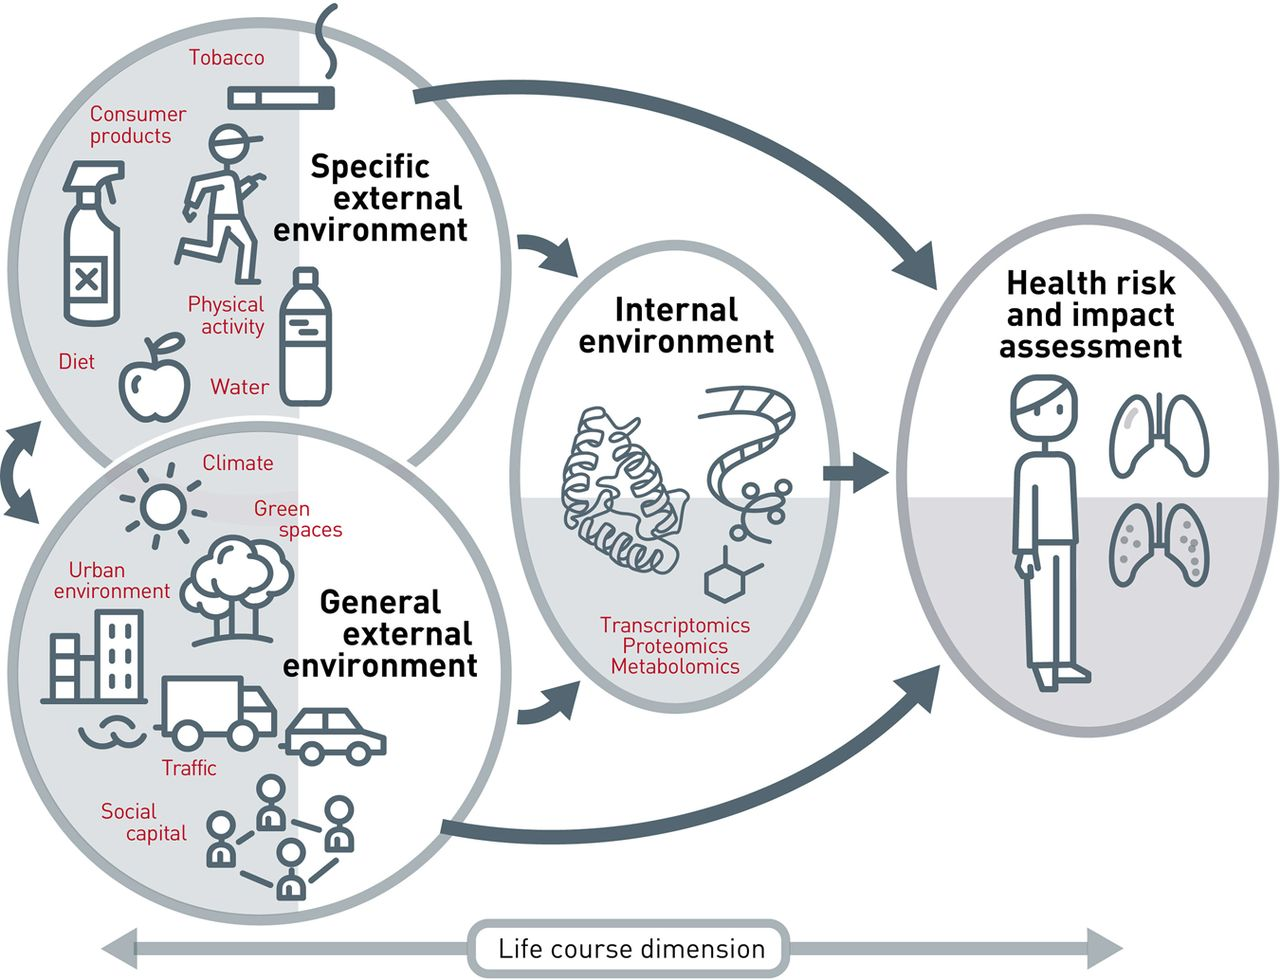
\includegraphics{images/exposome.jpg}
\caption{Vrijheid et al.~Thorax. 2014}
\end{figure}

The following DAG presents an integrative framework for environmental exposures (E), lifestyle and behavioral factors (B), and social constructs (X), which may be complex but has the potential to elucidate mechanisms through which diseases are caused, which we presented in an introductory publication (\citet{bellavia2018multiple}).

\begin{figure}
\centering
\includegraphics{images/mediation.png}
\caption{Bellavia et al.~Env. Epi. 2018}
\end{figure}

Integrating methods for environmental exposures into mediation analysis has been the goal of several recent papers, which the reader could refer to for further details (\citet{bellavia2019approaches}), (\citet{blum2020challenges}), (\citet{devick2018bayesian}). These methods have been largely unexplored in applied studies and may represent a critical tool to further identify the mechanisms through which the exposome affects human health. A recent R function was also developed to integrate BKMR into a mediation analysis context (\citet{wang2020bkmr}).

\hypertarget{conclusion}{%
\section{Conclusion}\label{conclusion}}

The goal of this introductory course was to discuss the challenges involved in the study of environmental mixtures as they relate to health outcomes and introduce the most common statistical approaches that can help addressing some of these challenges. The core points of the discussion were the following:

\begin{itemize}
\item
  Environmental mixtures represent the way environmental exposures occur and operate in real life and, as such, should be integrated and evaluated in environmental epidemiology studies. This involves a series of analytic and statistical issues that should be carefully addressed and taken into account.
\item
  A first critical classification of statistical methodologies it the one between supervised and unsupervised approaches. It is always recommended to begin the analyses with a thorough pre-processing phase that involves unsupervised techniques. These will help identifying clustering and groupings of exposures, high levels of correlations, missingness, and the presence of inflated covariates, crucially guiding subsequent steps.
\item
  When incorporating the outcome into the picture (supervised approaches) it it always recommended to begin with regression-based approaches. These provide unique advantages and most of the times will provide a good fit to the question of interest.
\item
  Specific methods have been developed to address environmental mixtures when regression techniques are of little use or more flexible approaches are required. This occurs, for example, when high-dimensional interactions are of interests, if most associations are non-linear, or if the primary interest is in retrieving the cumulative mixture effect. Generally, all techniques come with some limitations and it is always recommended to test several methods and validate results providing different perspectives.
\item
  With a very large number of exposures and/or interaction, machine learning (ML) techniques should be considered. Recent extensions of random forests such as gradient boosting machines (or boosted regression trees) provide several advantages in this context. Proceeding with different layers of analysis, using ML results to build a second-step regression model is recommended.
\item
  Most current methods are available and well documented/presented in the statistical software R.
\item
  In general, when dealing with environmental exposures, the choice of the methods should be drive by the research question of interest.

  \begin{itemize}
  \tightlist
  \item
    Are there exposure patterns? (unsupervised analysis, e.g.~PCA)
  \item
    What are the effects of individual exposures within the mixture? (regression methods, BKMR)
  \item
    What are the most important contributors to the association? (PIPs in BKMR, weights from WQS, selected covariates in elastic net \ldots)
  \item
    What is the overall (cumulative) effect of the mixture? (regression methods, WQS)
  \item
    Are there interactions (or even synergy) between chemicals? (tree-based modeling, BKMR, regression methods)
  \end{itemize}
\end{itemize}

Several papers have been presented discussing all these techniques and providing further guidance to choose the correct approach (\citet{hamra2018environmental}),(\citet{stafoggia2017statistical}),(\citet{gibson2019overview}). Finally, it is useful to remind that the material here presented is just a selection of topics out of a wide and fast-growing research area. Methodological extensions and new applications are continuously published and it is crucial for researchers working in this area to keep up with the literature.

  \bibliography{book.bib,packages.bib}

\end{document}
